\chapter{模型压缩及移动端部署}\label{ux7b2cux5341ux4e03ux7ae0-ux6a21ux578bux538bux7f29ux53caux79fbux52a8ux7aefux90e8ux7f72}

​
深度神经网络在人工智能的应用中,包括语音识别、计算机视觉、自然语言处理等各方面,在取得巨大成功的同时,这些深度神经网络需要巨大的计算开销和内存开销,严重阻碍了资源受限下的使用。本章总结了模型压缩、加速一般原理和方法,以及在移动端如何部署。

\subsection{模型压缩理解}\label{ux6a21ux578bux538bux7f29ux7406ux89e3}

​
模型压缩是指利用数据集对已经训练好的深度模型进行精简,进而得到一个轻量且准确率相当的网络,压缩后的网络具有更小的结构和更少的参数,可以有效降低计算和存储开销,便于部署再受限的硬件环境中。

\subsection{为什么需要模型压缩和加速?}\label{ux4e3aux4ec0ux4e48ux9700ux8981ux6a21ux578bux538bux7f29ux548cux52a0ux901f}

(1)随着AI技术的飞速发展,越来越多的公司希望在自己的移动端产品中注入AI能力。

(2)对于在线学习和增量学习等实时应用而言,如何减少含有大量层级及结点的大型神经网络所需要的内存和计算量显得极为重要。

(3)模型的参数在一定程度上能够表达其复杂性,相关研究表明,并不是所有的参数都在模型中发挥作用,部分参数作用有限、表达冗余,甚至会降低模型的性能。

(4)复杂的模型固然具有更好的性能,但是高额的存储空间、计算资源消耗是使其难以有效的应用在各硬件平台上的重要原因。

(5)智能设备的流行提供了内存、CPU、能耗和宽带等资源,使得深度学习模型部署在智能移动设备上变得可行。\\
(6)高效的深度学习方法可以有效的帮助嵌入式设备、分布式系统完成复杂工作,在移动端部署深度学习有很重要的意义。

\subsection{17.3
模型压缩的必要性及可行性}\label{ux6a21ux578bux538bux7f29ux7684ux5fc5ux8981ux6027ux53caux53efux884cux6027}

\begin{longtable}[]{ ll }
\toprule
\begin{minipage}[b]{0.12\columnwidth}\raggedright\strut
必要性\strut
\end{minipage} & \begin{minipage}[b]{0.80\columnwidth}\raggedright\strut
首先是资源受限,其次在许多网络结构中,如VGG-16网络,参数数量1亿3千多万,占用500MB空间,需要进行309亿次浮点运算才能完成一次图像识别任务。\strut
\end{minipage}\tabularnewline
\midrule
\endhead
\begin{minipage}[t]{0.12\columnwidth}\raggedright\strut
可行性\strut
\end{minipage} & \begin{minipage}[t]{0.80\columnwidth}\raggedright\strut
模型的参数在一定程度上能够表达其复杂性,相关研究表明,并不是所有的参数都在模型中发挥作用,部分参数作用有限、表达冗余,甚至会降低模型的性能。论文提出,很多的深度神经网络仅仅使用很少一部分(5\%)权值就足以预测剩余的权值。该论文还提出这些剩下的权值甚至可以直接不用被学习。也就是说,仅仅训练一小部分原来的权值参数就有可能达到和原来网络相近甚至超过原来网络的性能(可以看作一种正则化)。\strut
\end{minipage}\tabularnewline
\begin{minipage}[t]{0.12\columnwidth}\raggedright\strut
最终目的\strut
\end{minipage} & \begin{minipage}[t]{0.80\columnwidth}\raggedright\strut
最大程度的减小模型复杂度,减少模型存储需要的空间,也致力于加速模型的训练和推测\strut
\end{minipage}\tabularnewline
\bottomrule
\end{longtable}

\subsection{17.4
目前有哪些深度学习模型压缩方法?}\label{ux76eeux524dux6709ux54eaux4e9bux6df1ux5ea6ux5b66ux4e60ux6a21ux578bux538bux7f29ux65b9ux6cd5}

​
目前深度学习模型压缩方法主要分为更精细化模型设计、模型裁剪、核的稀疏化、量化、低秩分解、迁移学习等方法,而这些方法又可分为前端压缩和后端压缩。

\subsubsection{17.4.1
前端压缩和后端压缩对比}\label{ux524dux7aefux538bux7f29ux548cux540eux7aefux538bux7f29ux5bf9ux6bd4}

\begin{longtable}[]{ ccc }
\toprule
对比项目 & 前端压缩 & 后端压缩\tabularnewline
\midrule
\endhead
含义 & 不会改变原始网络结构的压缩技术 &
会大程度上改变原始网络结构的压缩技术\tabularnewline
主要方法 & 知识蒸馏、紧凑的模型结构设计、滤波器层面的剪枝 &
低秩近似、未加限制的剪枝、参数量化、二值网络\tabularnewline
实现难度 & 较简单 & 较难\tabularnewline
是否可逆 & 可逆 & 不可逆\tabularnewline
成熟应用 & 剪枝 & 低秩近似、参数量化\tabularnewline
待发展应用 & 知识蒸馏 & 二值网络\tabularnewline
\bottomrule
\end{longtable}

\subsubsection{17.4.2 网络剪枝}\label{ux7f51ux7edcux526aux679d}

深度学习模型因其\textbf{稀疏性},可以被裁剪为结构精简的网络模型,具体包括结构性剪枝与非结构性剪枝。

\begin{longtable}[]{ lll }
\toprule
\begin{minipage}[b]{0.09\columnwidth}\raggedright\strut
事项\strut
\end{minipage} & \begin{minipage}[b]{0.41\columnwidth}\raggedright\strut
特点\strut
\end{minipage} & \begin{minipage}[b]{0.41\columnwidth}\raggedright\strut
举例\strut
\end{minipage}\tabularnewline
\midrule
\endhead
\begin{minipage}[t]{0.09\columnwidth}\raggedright\strut
非结构化剪枝\strut
\end{minipage} & \begin{minipage}[t]{0.41\columnwidth}\raggedright\strut
通常是连接级、细粒度的剪枝方法,精度相对较高,但依赖于特定算法库或硬件平台的支持\strut
\end{minipage} & \begin{minipage}[t]{0.41\columnwidth}\raggedright\strut
Deep Compression {[}5{]}, Sparse-Winograd {[}6{]} 算法等;\strut
\end{minipage}\tabularnewline
\begin{minipage}[t]{0.09\columnwidth}\raggedright\strut
结构化剪枝\strut
\end{minipage} & \begin{minipage}[t]{0.41\columnwidth}\raggedright\strut
是filter级或layer级、粗粒度的剪枝方法,精度相对较低,但剪枝策略更为有效,不需要特定算法库或硬件平台的支持,能够直接在成熟深度学习框架上运行。\strut
\end{minipage} & \begin{minipage}[t]{0.41\columnwidth}\raggedright\strut
如局部方式的、通过layer by layer方式的、最小化输出FM重建误差的Channel
Pruning {[}7{]}, ThiNet {[}8{]}, Discrimination-aware Channel Pruning
{[}9{]};全局方式的、通过训练期间对BN层Gamma系数施加L1正则约束的Network
Slimming {[}10{]};全局方式的、按Taylor准则对Filter作重要性排序的Neuron
Pruning {[}11{]};全局方式的、可动态重新更新pruned filters参数的剪枝方法
{[}12{]};https://blog.csdn.net/baidu\_31437863/article/details/84474847\strut
\end{minipage}\tabularnewline
\bottomrule
\end{longtable}

如果按剪枝粒度分,从粗到细,可分为中间隐含层剪枝、通道剪枝、卷积核剪枝、核内剪枝、单个权重剪枝。下面按照剪枝粒度的分类从粗(左)到细(右)。

\begin{figure}
\centering
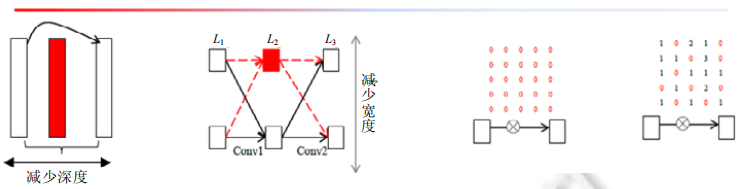
\includegraphics{./img/ch17/剪枝粒度分类.png}
\caption{}
\end{figure}

(a)层间剪枝 (b)特征图剪枝 (c)k*k核剪枝 (d)核内剪枝

\begin{longtable}[]{ ll }
\toprule
\begin{minipage}[b]{0.24\columnwidth}\raggedright\strut
事项\strut
\end{minipage} & \begin{minipage}[b]{0.70\columnwidth}\raggedright\strut
特点\strut
\end{minipage}\tabularnewline
\midrule
\endhead
\begin{minipage}[t]{0.24\columnwidth}\raggedright\strut
单个权重粒度\strut
\end{minipage} & \begin{minipage}[t]{0.70\columnwidth}\raggedright\strut
早期 Le Cun{[}16{]}提出的 OBD(optimal brain
damage)将网络中的任意权重参数都看作单个参数,能够有效地提高预测准确率,却不能减小运行时间;同时,剪枝代价过高,只适用于小网络\strut
\end{minipage}\tabularnewline
\begin{minipage}[t]{0.24\columnwidth}\raggedright\strut
核内权重粒度\strut
\end{minipage} & \begin{minipage}[t]{0.70\columnwidth}\raggedright\strut
网络中的任意权重被看作是单个参数并进行随机非结构化剪枝,该粒度的剪枝导致网络连接不规整,需要通过稀疏表达来减少内存占用,进而导致在前向传播预测时,需要大量的条件判断和额外空间来标明零或非零参数的位置,因此不适用于并行计算\strut
\end{minipage}\tabularnewline
\begin{minipage}[t]{0.24\columnwidth}\raggedright\strut
卷积核粒度与通道粒度\strut
\end{minipage} & \begin{minipage}[t]{0.70\columnwidth}\raggedright\strut
卷积核粒度与通道粒度属于粗粒度剪枝,不依赖任何稀疏卷积计算库及专用硬件;同时,能够在获得高压缩率的同时大量减小测试阶段的计算时间.由\strut
\end{minipage}\tabularnewline
\bottomrule
\end{longtable}

从剪枝目标上分类,可分为减少参数/网络复杂度、减少过拟合/增加泛化能力/提高准确率、减小部署运行时间/提高网络效率及减小训练时间等。

\subsubsection{17.4.3
典型剪枝方法对比}\label{ux5178ux578bux526aux679dux65b9ux6cd5ux5bf9ux6bd4}

\begin{longtable}[]{ cccc }
\toprule
剪枝方法 & 修剪对象 & 修剪方式 & 效果\tabularnewline
\midrule
\endhead
Deep Compression & 权重 & 随机修剪 & 50倍压缩\tabularnewline
Structured Pruning & 权重 & 组稀疏+排他性稀疏 & 性能提升\tabularnewline
Network Slimming & 特征图通道 & 根据尺度因子修剪 &
节省计算资源\tabularnewline
mProp & 梯度 & 修剪幅值小的梯度 & 加速\tabularnewline
\bottomrule
\end{longtable}

\subsubsection{17.4.4 网络蒸馏}\label{ux7f51ux7edcux84b8ux998f}

​ 网络精馏是指利用大量未标记的迁移数据(transfer
data),让小模型去拟合大模型,从而让小模型学到与大模型相似的函数映射.网络精馏可以看成在同一个域上迁移学习{[}34{]}的一种特例,目的是获得一个比原模型更为精简的网络,整体的框架图如图
4所示.

\begin{figure}
\centering
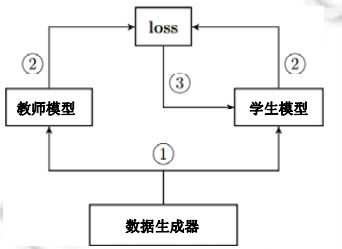
\includegraphics{./img/ch17/网络蒸馏.png}
\caption{}
\end{figure}

\subsubsection{17.4.5 前端压缩}\label{ux524dux7aefux538bux7f29}

(1)知识蒸馏

​
一个复杂模型可由多个简单模型或者强约束条件训练得到。复杂模型特点是性能好,但其参数量大,计算效率低。小模型特点是计算效率高,但是其性能较差。知识蒸馏是让复杂模型学习到的知识迁移到小模型当中,使其保持其快速的计算速度前提下,同时拥有复杂模型的性能,达到模型压缩的目的。
(2)紧凑的模型结构设计\\
​
紧凑的模型结构设计主要是对神经网络卷积的方式进行改进,比如使用两个3x3的卷积替换一个5x5的卷积、使用深度可分离卷积等等方式降低计算参数量。
目前很多网络基于模块化设计思想,在深度和宽度两个维度上都很大,导致参数冗余。因此有很多关于模型设计的研究,如SqueezeNet、MobileNet等,使用更加细致、高效的模型设计,能够很大程度的减少模型尺寸,并且也具有不错的性能。\\
(3)滤波器层面的剪枝\\
​
滤波器层面的剪枝属于非结构花剪枝,主要是对较小的权重矩阵整个剔除,然后对整个神经网络进行微调。此方式由于剪枝过于粗放,容易导致精度损失较大,而且部分权重矩阵中会存留一些较小的权重造成冗余,剪枝不彻底。
具体操作是在训练时使用稀疏约束(加入权重的稀疏正则项,引导模型的大部分权重趋向于0)。完成训练后,剪去滤波器上的这些
0 。

​ 优点是简单,缺点是剪得不干净,非结构化剪枝会增加内存访问成本。

\subsubsection{17.4.6 后端压缩}\label{ux540eux7aefux538bux7f29}

(1)低秩近似\\
​
在卷积神经网络中,卷积运算都是以矩阵相乘的方式进行。对于复杂网络,权重矩阵往往非常大,非常消耗存储和计算资源。低秩近似就是用若干个低秩矩阵组合重构大的权重矩阵,以此降低存储和计算资源消耗。

\begin{longtable}[]{ ll }
\toprule
\begin{minipage}[b]{0.07\columnwidth}\raggedright\strut
事项\strut
\end{minipage} & \begin{minipage}[b]{0.80\columnwidth}\raggedright\strut
特点\strut
\end{minipage}\tabularnewline
\midrule
\endhead
\begin{minipage}[t]{0.07\columnwidth}\raggedright\strut
优点\strut
\end{minipage} & \begin{minipage}[t]{0.80\columnwidth}\raggedright\strut
可以降低存储和计算消耗;一般可以压缩2-3倍;精度几乎没有损失;\strut
\end{minipage}\tabularnewline
\begin{minipage}[t]{0.07\columnwidth}\raggedright\strut
缺点\strut
\end{minipage} & \begin{minipage}[t]{0.80\columnwidth}\raggedright\strut
模型越复杂,权重矩阵越大,利用低秩近似重构参数矩阵不能保证模型的性能 ;
超参数的数量随着网络层数的增加呈线性变化趋势,例如中间层的特征通道数等等。
随着模型复杂度的提升,搜索空间急剧增大。\strut
\end{minipage}\tabularnewline
\bottomrule
\end{longtable}

(2)未加限制的剪枝

​ 完成训练后,不加限制地剪去那些冗余参数。

\begin{longtable}[]{ ll }
\toprule
事项 & 特点\tabularnewline
\midrule
\endhead
优点 & 保持模型性能不损失的情况下,减少参数量9-11倍;
剔除不重要的权重,可以加快计算速度,同时也可以提高模型的泛化能力;\tabularnewline
缺点 & 极度依赖专门的运行库和特殊的运行平台,不具有通用性;
压缩率过大时,破坏性能;\tabularnewline
\bottomrule
\end{longtable}

(3)参数量化

​
神经网络的参数类型一般是32位浮点型,使用较小的精度代替32位所表示的精度。或者是将多个权重映射到同一数值,权重共享。\textbf{量化其实是一种权值共享的策略}。量化后的权值张量是一个高度稀疏的有很多共享权值的矩阵,对非零参数,我们还可以进行定点压缩,以获得更高的压缩率。

\begin{longtable}[]{ ll }
\toprule
\begin{minipage}[b]{0.07\columnwidth}\raggedright\strut
事项\strut
\end{minipage} & \begin{minipage}[b]{0.80\columnwidth}\raggedright\strut
特点\strut
\end{minipage}\tabularnewline
\midrule
\endhead
\begin{minipage}[t]{0.07\columnwidth}\raggedright\strut
优点\strut
\end{minipage} & \begin{minipage}[t]{0.80\columnwidth}\raggedright\strut
模型性能损失很小,大小减少8-16倍;\strut
\end{minipage}\tabularnewline
\begin{minipage}[t]{0.07\columnwidth}\raggedright\strut
缺点\strut
\end{minipage} & \begin{minipage}[t]{0.80\columnwidth}\raggedright\strut
压缩率大时,性能显著下降; 依赖专门的运行库,通用性较差;\strut
\end{minipage}\tabularnewline
\begin{minipage}[t]{0.07\columnwidth}\raggedright\strut
举例\strut
\end{minipage} & \begin{minipage}[t]{0.80\columnwidth}\raggedright\strut
二值化网络:XNORnet {[}13{]}, ABCnet with Multiple Binary Bases
{[}14{]}, Bin-net with High-Order Residual Quantization {[}15{]},
Bi-Real Net {[}16{]};三值化网络:Ternary weight networks {[}17{]},
Trained Ternary Quantization {[}18{]};\strut
\end{minipage}\tabularnewline
\bottomrule
\end{longtable}

W1-A8 或 W2-A8量化: Learning Symmetric Quantization {[}19{]};
INT8量化:TensorFlow-lite {[}20{]}, TensorRT {[}21{]};
其他(非线性):Intel INQ {[}22{]}, log-net, CNNPack {[}23{]} 等;
原文:https://blog.csdn.net/baidu\_31437863/article/details/84474847
\textbar{} \textbar{} 总结 \textbar{}
最为典型就是二值网络、XNOR网络等。其主要原理就是采用1bit对网络的输入、权重、响应进行编码。减少模型大小的同时,原始网络的卷积操作可以被bit-wise运算代替,极大提升了模型的速度。但是,如果原始网络结果不够复杂(模型描述能力),由于二值网络会较大程度降低模型的表达能力。因此现阶段有相关的论文开始研究n-bit编码方式成为n值网络或者多值网络或者变bit、组合bit量化来克服二值网络表达能力不足的缺点。
\textbar{}

(4)二值网络

​
相对量化更为极致,对于32bit浮点型数用1bit二进制数-1或者1表示,可大大减小模型尺寸。

\begin{longtable}[]{ ll }
\toprule
事项 & 特点\tabularnewline
\midrule
\endhead
优点 &
网络体积小,运算速度快,有时可避免部分网络的overfitting\tabularnewline
缺点 &
二值神经网络损失的信息相对于浮点精度是非常大;粗糙的二值化近似导致训练时模型收敛速度非常慢\tabularnewline
\bottomrule
\end{longtable}

(5)三值网络

\begin{longtable}[]{ ll }
\toprule
\begin{minipage}[b]{0.07\columnwidth}\raggedright\strut
事项\strut
\end{minipage} & \begin{minipage}[b]{0.80\columnwidth}\raggedright\strut
特点\strut
\end{minipage}\tabularnewline
\midrule
\endhead
\begin{minipage}[t]{0.07\columnwidth}\raggedright\strut
优点\strut
\end{minipage} & \begin{minipage}[t]{0.80\columnwidth}\raggedright\strut
相对于二值神经网络,三值神经网络(Ternary Weight
Networks)在同样的模型结构下可以达到成百上千倍的表达能力提升;并且,在计算时间复杂度上,三元网络和二元网络的计算复杂度是一样的。例如,对于ResNet-18层网络中最常出现的卷积核(3x3大小),二值神经网络模型最多可以表达2的3x3次方(=512)种结构,而三元神经网络则可以表达3的3x3次方(=19683)种卷积核结构。在表达能力上,三元神经网络相对要高19683/512
=
38倍。因此,三元神经网络模型能够在保证计算复杂度很低的情况下大幅的提高网络的表达能力,进而可以在精度上相对于二值神经网络有质的飞跃。另外,由于对中间信息的保存更多,三元神经网络可以极大的加快网络训练时的收敛速度,从而更快、更稳定的达到最优的结果。\strut
\end{minipage}\tabularnewline
\begin{minipage}[t]{0.07\columnwidth}\raggedright\strut
\strut
\end{minipage} & \begin{minipage}[t]{0.80\columnwidth}\raggedright\strut
\strut
\end{minipage}\tabularnewline
\bottomrule
\end{longtable}

\subsubsection{17.4.6 低秩分解}\label{ux4f4eux79e9ux5206ux89e3}

基于低秩分解的深度神经网络压缩与加速的核心思想是利用矩阵或张量分解技术估计并分解深度模型中的原始卷积核.卷积计算是整个卷积神经网络中计算复杂
度 最 高 的 计 算 操 作,通 过 分 解4D
卷积核张量,可以有效地减少模型内部的冗余性.此外对于2D的全 连 接 层 矩
阵 参
数,同样可以利用低秩分解技术进行处理.但由于卷积层与全连接层的分解方式不同,本文分别从卷积层和全连接层2个不同角度回顾与分析低秩分解技术在深度神经网络中的应用.

在2013年,Denil等人[57]从理论上利用低秩分解的技术并分析了深度神经网络存在大量的冗余信
息,开创了基于低秩分解的深度网络模型压缩与加速的新思路.如图7所示,展示了主流的张量分解后卷积
计 算.

\begin{figure}
\centering
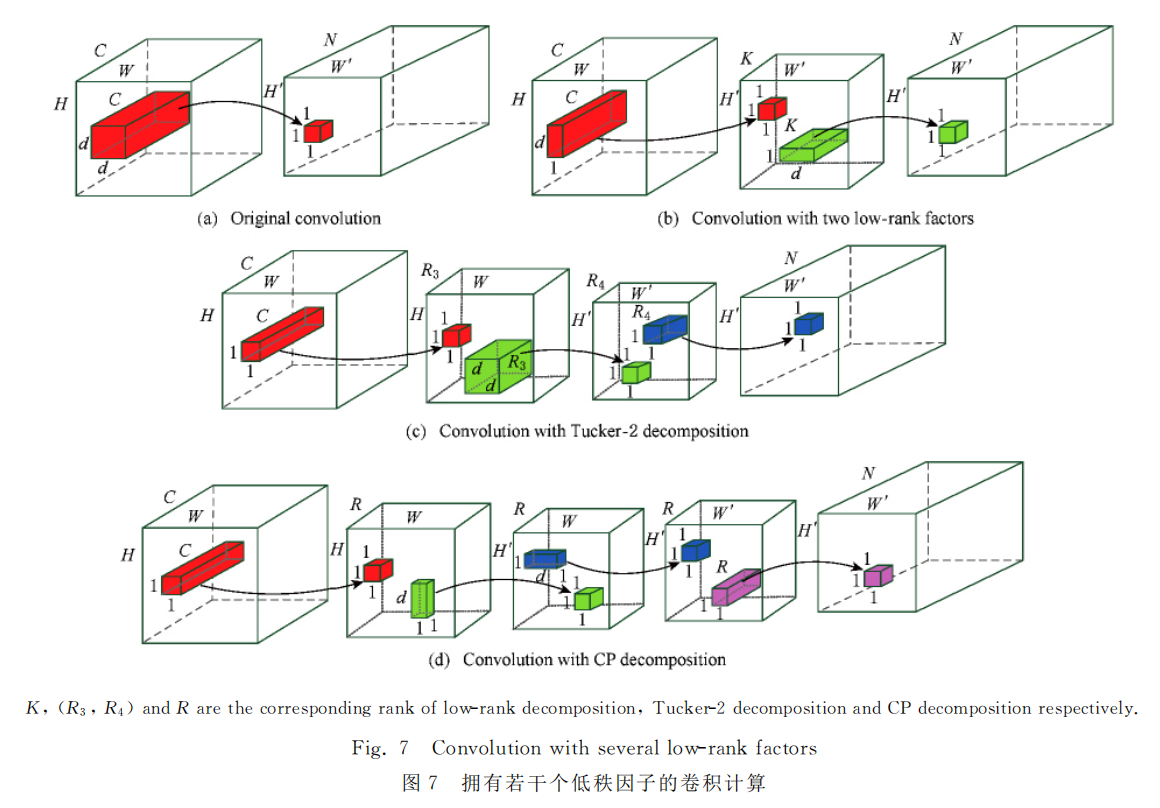
\includegraphics{./img/ch17/低秩分解模型压缩加速.jpg}
\caption{}
\end{figure}

(出自《深度神经网络压缩与加速综述》)

\subsubsection{17.4.7
总体压缩效果评价指标有哪些?}\label{ux603bux4f53ux538bux7f29ux6548ux679cux8bc4ux4ef7ux6307ux6807ux6709ux54eaux4e9b}

​
网络压缩评价指标包括运行效率、参数压缩率、准确率.与基准模型比较衡量性能提升时,可以使用提升倍数(speedup)或提升比例(ratio)。

\begin{longtable}[]{ ll }
\toprule
评价指标 & 特点\tabularnewline
\midrule
\endhead
准确率 & 目前,大部分研究工作均会测量 Top-1 准确率,只有在 ImageNet
这类大型数据集上才会只用 Top-5 准确率.为方便比较\tabularnewline
参数压缩率 &
统计网络中所有可训练的参数,根据机器浮点精度转换为字节(byte)量纲,通常保留两位有效数字以作近似估计.\tabularnewline
运行效率 &
可以从网络所含浮点运算次数(FLOP)、网络所含乘法运算次数(MULTS)或随机实验测得的网络平均前向传播所需时间这
3 个角度来评价\tabularnewline
\bottomrule
\end{longtable}

\subsubsection{17.4.8
几种轻量化网络结构对比}\label{ux51e0ux79cdux8f7bux91cfux5316ux7f51ux7edcux7ed3ux6784ux5bf9ux6bd4}

\begin{longtable}[]{ cccc }
\toprule
网络结构 & TOP1 准确率/\% & 参数量/M & CPU运行时间/ms\tabularnewline
\midrule
\endhead
MobileNet V1 & 70.6 & 4.2 & 123\tabularnewline
ShuffleNet(1.5) & 69.0 & 2.9 & -\tabularnewline
ShuffleNet(x2) & 70.9 & 4.4 & -\tabularnewline
MobileNet V2 & 71.7 & 3.4 & 80\tabularnewline
MobileNet V2(1.4) & 74.7 & 6.9 & 149\tabularnewline
\bottomrule
\end{longtable}

\subsubsection{17.4.9
网络压缩未来研究方向有哪些?}\label{ux7f51ux7edcux538bux7f29ux672aux6765ux7814ux7a76ux65b9ux5411ux6709ux54eaux4e9b}

网络剪枝、网络精馏和网络分解都能在一定程度上实现网络压缩的目的.回归到深度网络压缩的本质目的上,即提取网络中的有用信息,以下是一些值得研究和探寻的方向.
(1)
权重参数对结果的影响度量.深度网络的最终结果是由全部的权重参数共同作用形成的,目前,关于单个卷积核/卷积核权重的重要性的度量仍然是比较简单的方式,尽管文献{[}14{]}中给出了更为细节的分析,但是由于计算难度大,并不实用.因此,如何通过更有效的方式来近似度量单个参数对模型的影响,具有重要意义.
(2)
学生网络结构的构造.学生网络的结构构造目前仍然是由人工指定的,然而,不同的学生网络结构的训练难度不同,最终能够达到的效果也有差异.因此,如何根据教师网络结构设计合理的网络结构在精简模型的条件下获取较高的模型性能,是未来的一个研究重点.
(3)
参数重建的硬件架构支持.通过分解网络可以无损地获取压缩模型,在一些对性能要求高的场景中是非常重要的.然而,参数的重建步骤会拖累预测阶段的时间开销,如何通过硬件的支持加速这一重建过程,将是未来的一个研究方向.
(4)
任务或使用场景层面的压缩.大型网络通常是在量级较大的数据集上训练完成的,比如,在
ImageNet上训练的模型具备对 1 000
类物体的分类,但在一些具体场景的应用中,可能仅需要一个能识别其中几类的小型模型.因此,如何从一个全功能的网络压缩得到部分功能的子网络,能够适应很多实际应用场景的需求.
(5)
网络压缩效用的评价.目前,对各类深度网络压缩算法的评价是比较零碎的,侧重于和被压缩的大型网络在参数量和运行时间上的比较.未来的研究可以从提出更加泛化的压缩评价标准出发,一方面平衡运行速度和模型大小在不同应用场景下的影响;另一方面,可以从模型本身的结构性出发,对压缩后的模型进行评价.

(出自《深度网络模型压缩综述》)

\subsection{17.5
目前有哪些深度学习模型优化加速方法?}\label{ux76eeux524dux6709ux54eaux4e9bux6df1ux5ea6ux5b66ux4e60ux6a21ux578bux4f18ux5316ux52a0ux901fux65b9ux6cd5}

https://blog.csdn.net/nature553863/article/details/81083955

\subsubsection{17.5.1
模型优化加速方法}\label{ux6a21ux578bux4f18ux5316ux52a0ux901fux65b9ux6cd5}

模型优化加速能够提升网络的计算效率,具体包括:\\
(1)Op-level的快速算法:FFT Conv2d (7x7, 9x9), Winograd Conv2d (3x3,
5x5) 等;\\
(2)Layer-level的快速算法:Sparse-block net {[}1{]} 等;\\
(3)优化工具与库:TensorRT (Nvidia), Tensor Comprehension (Facebook) 和
Distiller (Intel) 等;

原文:https://blog.csdn.net/nature553863/article/details/81083955

\subsubsection{17.5.2
TensorRT加速原理}\label{tensorrtux52a0ux901fux539fux7406}

https://blog.csdn.net/xh\_hit/article/details/79769599

​
在计算资源并不丰富的嵌入式设备上,TensorRT之所以能加速神经网络的的推断主要得益于两点:

\begin{itemize}
\item
  首先是TensorRT支持int8和fp16的计算,通过在减少计算量和保持精度之间达到一个理想的trade-off,达到加速推断的目的。
\item
  更为重要的是TensorRT对于网络结构进行了重构和优化,主要体现在一下几个方面。
\end{itemize}

\begin{enumerate}
\def\labelenumi{(\arabic{enumi})}
\item
  TensorRT通过解析网络模型将网络中无用的输出层消除以减小计算。
\item
  对于网络结构的垂直整合,即将目前主流神经网络的Conv、BN、Relu三个层融合为了一个层,例如将图1所示的常见的Inception结构重构为图2所示的网络结构。
\item
  对于网络结构的水平组合,水平组合是指将输入为相同张量和执行相同操作的层融合一起,例如图2向图3的转化。
\end{enumerate}

\begin{figure}
\centering
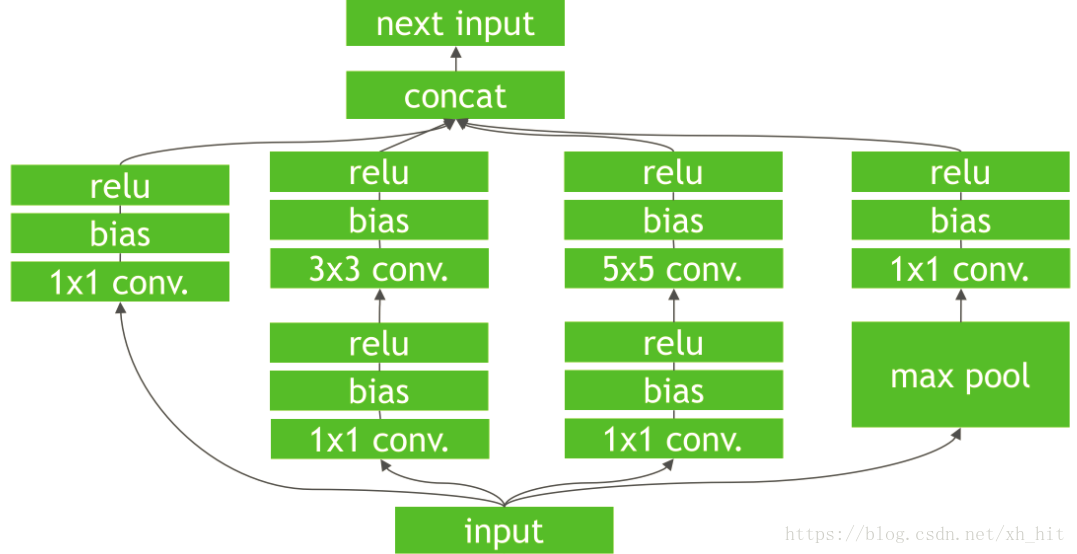
\includegraphics{./img/ch17/tensorRT1.png}
\caption{}
\end{figure}

\begin{figure}
\centering
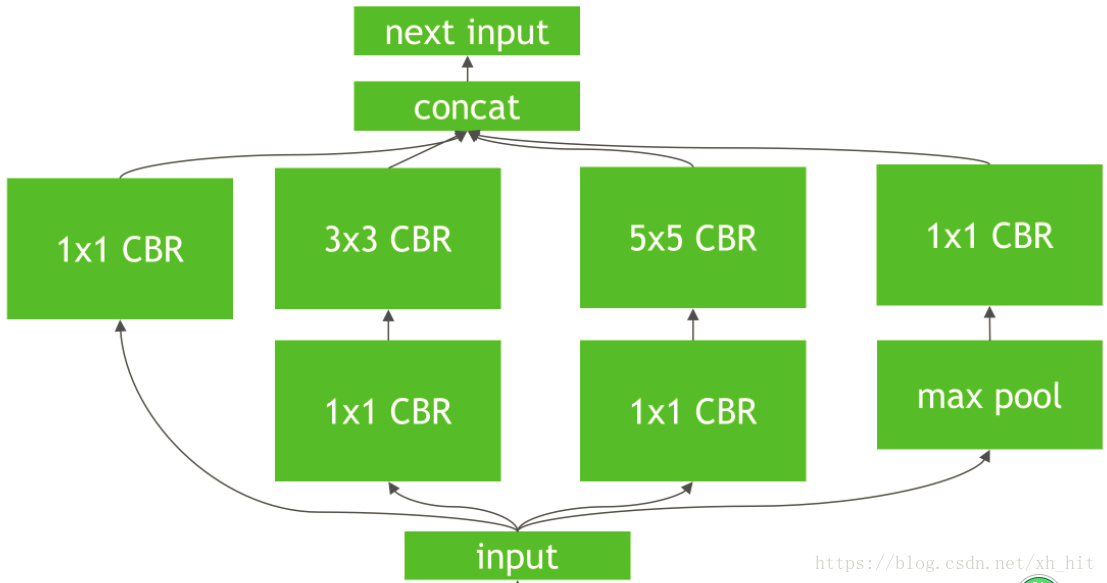
\includegraphics{./img/ch17/tensorRT2.png}
\caption{}
\end{figure}

\begin{figure}
\centering
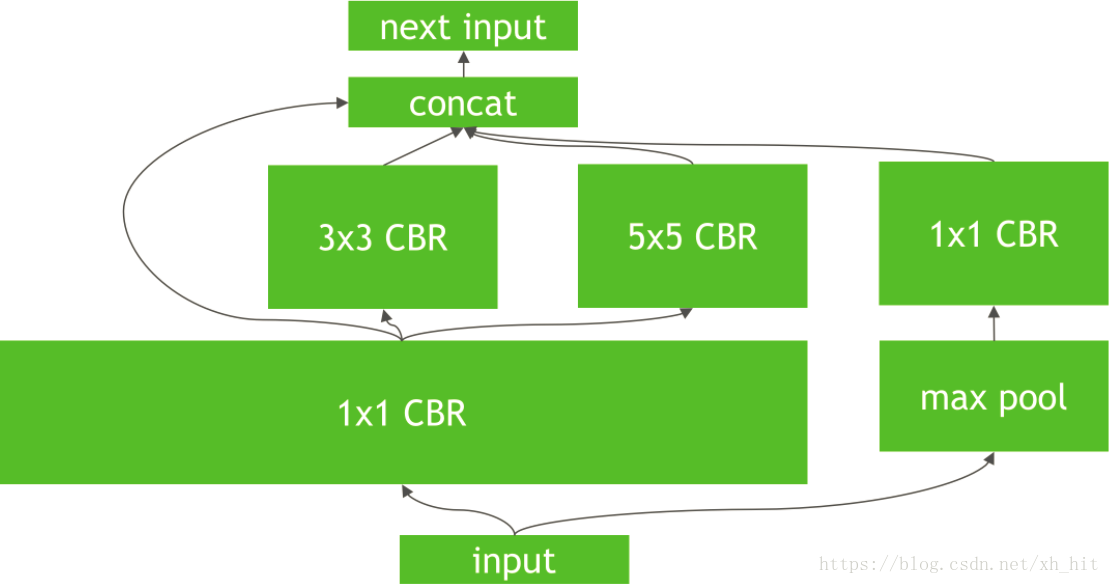
\includegraphics{./img/ch17/tensorRT3.png}
\caption{}
\end{figure}

​
以上3步即是TensorRT对于所部署的深度学习网络的优化和重构,根据其优化和重构策略,第一和第二步适用于所有的网络架构,但是第三步则对于含有Inception结构的神经网络加速效果最为明显。

​ Tips:
想更好地利用TensorRT加速网络推断,可在基础网络中多采用Inception模型结构,充分发挥TensorRT的优势。

\subsubsection{17.5.3
TensorRT如何优化重构模型?}\label{tensorrtux5982ux4f55ux4f18ux5316ux91cdux6784ux6a21ux578b}

\begin{longtable}[]{ ll }
\toprule
\begin{minipage}[b]{0.38\columnwidth}\raggedright\strut
条件\strut
\end{minipage} & \begin{minipage}[b]{0.56\columnwidth}\raggedright\strut
方法\strut
\end{minipage}\tabularnewline
\midrule
\endhead
\begin{minipage}[t]{0.38\columnwidth}\raggedright\strut
若训练的网络模型包含TensorRT支持的操作\strut
\end{minipage} & \begin{minipage}[t]{0.56\columnwidth}\raggedright\strut
1、对于Caffe与TensorFlow训练的模型,若包含的操作都是TensorRT支持的,则可以直接由TensorRT优化重构\strut
\end{minipage}\tabularnewline
\begin{minipage}[t]{0.38\columnwidth}\raggedright\strut
\strut
\end{minipage} & \begin{minipage}[t]{0.56\columnwidth}\raggedright\strut
2、对于MXnet,
PyTorch或其他框架训练的模型,若包含的操作都是TensorRT支持的,可以采用TensorRT
API重建网络结构,并间接优化重构;\strut
\end{minipage}\tabularnewline
\begin{minipage}[t]{0.38\columnwidth}\raggedright\strut
若训练的网络模型包含TensorRT不支持的操作\strut
\end{minipage} & \begin{minipage}[t]{0.56\columnwidth}\raggedright\strut
1、TensorFlow模型可通过tf.contrib.tensorrt转换,其中不支持的操作会保留为TensorFlow计算节点;\strut
\end{minipage}\tabularnewline
\begin{minipage}[t]{0.38\columnwidth}\raggedright\strut
\strut
\end{minipage} & \begin{minipage}[t]{0.56\columnwidth}\raggedright\strut
2、不支持的操作可通过Plugin API实现自定义并添加进TensorRT计算图;\strut
\end{minipage}\tabularnewline
\begin{minipage}[t]{0.38\columnwidth}\raggedright\strut
\strut
\end{minipage} & \begin{minipage}[t]{0.56\columnwidth}\raggedright\strut
3、将深度网络划分为两个部分,一部分包含的操作都是TensorRT支持的,可以转换为TensorRT计算图。另一部则采用其他框架实现,如MXnet或PyTorch;\strut
\end{minipage}\tabularnewline
\bottomrule
\end{longtable}

\subsubsection{17.5.4
TensorRT加速效果如何?}\label{tensorrtux52a0ux901fux6548ux679cux5982ux4f55}

以下是在TitanX (Pascal)平台上,TensorRT对大型分类网络的优化加速效果:

\begin{longtable}[]{ ccccc }
\toprule
\begin{minipage}[b]{0.09\columnwidth}\centering\strut
Network\strut
\end{minipage} & \begin{minipage}[b]{0.09\columnwidth}\centering\strut
Precision\strut
\end{minipage} & \begin{minipage}[b]{0.20\columnwidth}\centering\strut
Framework/GPU:TitanXP\strut
\end{minipage} & \begin{minipage}[b]{0.24\columnwidth}\centering\strut
Avg.Time(Batch=8,unit:ms)\strut
\end{minipage} & \begin{minipage}[b]{0.24\columnwidth}\centering\strut
Top1 Val.Acc.(ImageNet-1k)\strut
\end{minipage}\tabularnewline
\midrule
\endhead
\begin{minipage}[t]{0.09\columnwidth}\centering\strut
Resnet50\strut
\end{minipage} & \begin{minipage}[t]{0.09\columnwidth}\centering\strut
fp32\strut
\end{minipage} & \begin{minipage}[t]{0.20\columnwidth}\centering\strut
TensorFlow\strut
\end{minipage} & \begin{minipage}[t]{0.24\columnwidth}\centering\strut
24.1\strut
\end{minipage} & \begin{minipage}[t]{0.24\columnwidth}\centering\strut
0.7374\strut
\end{minipage}\tabularnewline
\begin{minipage}[t]{0.09\columnwidth}\centering\strut
Resnet50\strut
\end{minipage} & \begin{minipage}[t]{0.09\columnwidth}\centering\strut
fp32\strut
\end{minipage} & \begin{minipage}[t]{0.20\columnwidth}\centering\strut
MXnet\strut
\end{minipage} & \begin{minipage}[t]{0.24\columnwidth}\centering\strut
15.7\strut
\end{minipage} & \begin{minipage}[t]{0.24\columnwidth}\centering\strut
0.7374\strut
\end{minipage}\tabularnewline
\begin{minipage}[t]{0.09\columnwidth}\centering\strut
Resnet50\strut
\end{minipage} & \begin{minipage}[t]{0.09\columnwidth}\centering\strut
fp32\strut
\end{minipage} & \begin{minipage}[t]{0.20\columnwidth}\centering\strut
TRT4.0.1\strut
\end{minipage} & \begin{minipage}[t]{0.24\columnwidth}\centering\strut
12.1\strut
\end{minipage} & \begin{minipage}[t]{0.24\columnwidth}\centering\strut
0.7374\strut
\end{minipage}\tabularnewline
\begin{minipage}[t]{0.09\columnwidth}\centering\strut
Resnet50\strut
\end{minipage} & \begin{minipage}[t]{0.09\columnwidth}\centering\strut
int8\strut
\end{minipage} & \begin{minipage}[t]{0.20\columnwidth}\centering\strut
TRT4.0.1\strut
\end{minipage} & \begin{minipage}[t]{0.24\columnwidth}\centering\strut
6\strut
\end{minipage} & \begin{minipage}[t]{0.24\columnwidth}\centering\strut
0.7226\strut
\end{minipage}\tabularnewline
\begin{minipage}[t]{0.09\columnwidth}\centering\strut
Resnet101\strut
\end{minipage} & \begin{minipage}[t]{0.09\columnwidth}\centering\strut
fp32\strut
\end{minipage} & \begin{minipage}[t]{0.20\columnwidth}\centering\strut
TensorFlow\strut
\end{minipage} & \begin{minipage}[t]{0.24\columnwidth}\centering\strut
36.7\strut
\end{minipage} & \begin{minipage}[t]{0.24\columnwidth}\centering\strut
0.7612\strut
\end{minipage}\tabularnewline
\begin{minipage}[t]{0.09\columnwidth}\centering\strut
Resnet101\strut
\end{minipage} & \begin{minipage}[t]{0.09\columnwidth}\centering\strut
fp32\strut
\end{minipage} & \begin{minipage}[t]{0.20\columnwidth}\centering\strut
MXnet\strut
\end{minipage} & \begin{minipage}[t]{0.24\columnwidth}\centering\strut
25.8\strut
\end{minipage} & \begin{minipage}[t]{0.24\columnwidth}\centering\strut
0.7612\strut
\end{minipage}\tabularnewline
\begin{minipage}[t]{0.09\columnwidth}\centering\strut
Resnet101\strut
\end{minipage} & \begin{minipage}[t]{0.09\columnwidth}\centering\strut
fp32\strut
\end{minipage} & \begin{minipage}[t]{0.20\columnwidth}\centering\strut
TRT4.0.1\strut
\end{minipage} & \begin{minipage}[t]{0.24\columnwidth}\centering\strut
19.3\strut
\end{minipage} & \begin{minipage}[t]{0.24\columnwidth}\centering\strut
0.7612\strut
\end{minipage}\tabularnewline
\begin{minipage}[t]{0.09\columnwidth}\centering\strut
Resnet101\strut
\end{minipage} & \begin{minipage}[t]{0.09\columnwidth}\centering\strut
int8\strut
\end{minipage} & \begin{minipage}[t]{0.20\columnwidth}\centering\strut
TRT4.0.1\strut
\end{minipage} & \begin{minipage}[t]{0.24\columnwidth}\centering\strut
9\strut
\end{minipage} & \begin{minipage}[t]{0.24\columnwidth}\centering\strut
0.7574\strut
\end{minipage}\tabularnewline
\bottomrule
\end{longtable}

\subsection{17.6
影响神经网络速度的4个因素(再稍微详细一点)}\label{ux5f71ux54cdux795eux7ecfux7f51ux7edcux901fux5ea6ux76844ux4e2aux56e0ux7d20ux518dux7a0dux5faeux8be6ux7ec6ux4e00ux70b9}

\begin{enumerate}
\def\labelenumi{\arabic{enumi}.}
\item
  FLOPs(FLOPs就是网络执行了多少multiply-adds操作);
\item
  MAC(内存访问成本);
\item
  并行度(如果网络并行度高,速度明显提升);
\item
  计算平台(GPU,ARM)
\end{enumerate}

\subsection{17.7
压缩和加速方法如何选择?}\label{ux538bux7f29ux548cux52a0ux901fux65b9ux6cd5ux5982ux4f55ux9009ux62e9}

​
1)对于在线计算内存存储有限的应用场景或设备,可以选择参数共享和参数剪枝方法,特别是二值量化权值和激活、结构化剪枝.其他方法虽然能够有效的压缩模型中的权值参数,但无法减小计算中隐藏的内存大小(如特征图).
​
2)如果在应用中用到的紧性模型需要利用预训练模型,那么参数剪枝、参数共享以及低秩分解将成为首要考虑的方法.相反地,若不需要借助预训练模型,则可以考虑紧性滤波设计及知识蒸馏方法.
​
3)若需要一次性端对端训练得到压缩与加速后模型,可以利用基于紧性滤波设计的深度神经网络压缩与加速方法.
​
4)一般情况下,参数剪枝,特别是非结构化剪枝,能大大压缩模型大小,且不容易丢失分类精度.对于需要稳定的模型分类的应用,非结构化剪枝成为首要选择.
​
5)若采用的数据集较小时,可以考虑知识蒸馏方法.对于小样本的数据集,学生网络能够很好地迁移教师模型的知识,提高学生网络的判别性.
​
6)主流的5个深度神经网络压缩与加速算法相互之间是正交的,可以结合不同技术进行进一步的压缩与加速.如:韩
松 等 人[30]结合了参数剪枝和参数共享;温伟等人[64]以及
Alvarez等人[85]结合了参数剪枝和低秩分解.此外对于特定的应用场景,如目标检测,可以对卷积层和全连接层使用不同的压缩与加速技术分别处理.

参考《深度神经网络压缩与加速综述》

\subsection{17.8
改变网络结构设计为什么会实现模型压缩、加速?}\label{ux6539ux53d8ux7f51ux7edcux7ed3ux6784ux8bbeux8ba1ux4e3aux4ec0ux4e48ux4f1aux5b9eux73b0ux6a21ux578bux538bux7f29ux52a0ux901f}

\subsubsection{17.8.1 Group convolution}\label{group-convolution}

​ Group
convolution最早出现在AlexNet中,是为了解决单卡显存不够,将网络部署到多卡上进行训练而提出。Group
convolution可以减少单个卷积1/g的参数量。如何计算的呢?

​ 假设

\begin{itemize}
% \tightlist
\item
  输入特征的的维度为\(H*W*C_1\);
\item
  卷积核的维度为\(H_1*W_1*C_1\),共\(C_2\)个;
\item
  输出特征的维度为\(H_1*W_1*C_2\) 。
\end{itemize}

传统卷积计算方式如下:\\
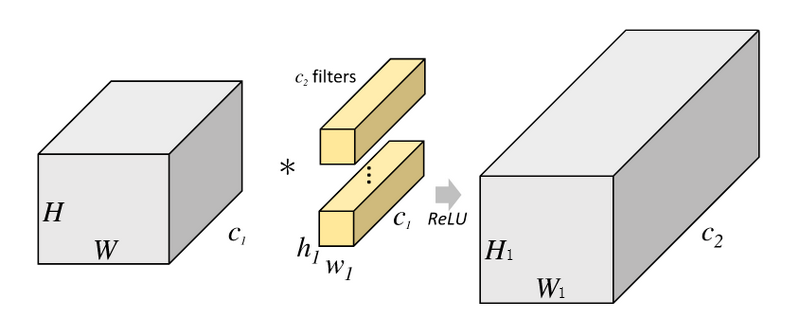
\includegraphics{./img/ch17/1.png} 传统卷积运算量为:\\
\[
A = H*W * h1 * w1 * c1 * c2
\] Group
convolution是将输入特征的维度c1分成g份,每个group对应的channel数为c1/g,特征维度H
* W * c1/g;,每个group对应的卷积核的维度也相应发生改变为h1 * w1 *
c1/9,共c2/g个;每个group相互独立运算,最后将结果叠加在一起。\\
Group convolution计算方式如下:\\
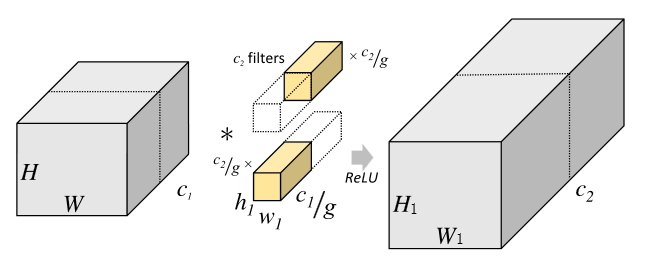
\includegraphics{./img/ch17/2.png} Group convolution运算量为:\\
\[
B = H * W * h1 * w1 * c1/g * c2/g * g
\] Group卷积相对于传统卷积的运算量:\\
\[
\dfrac{B}{A} = \dfrac{ H * W * h1 * w1 * c1/g * c2/g * g}{H * W * h1 * w1 * c1 * c2} = \dfrac{1}{g}
\] 由此可知:group卷积相对于传统卷积减少了1/g的参数量。

\subsubsection{17.8.2. Depthwise separable
convolution}\label{depthwise-separable-convolution}

Depthwise separable convolution是由depthwise conv和pointwise
conv构成。\\
depthwise conv(DW)有效减少参数数量并提升运算速度。但是由于每个feature
map只被一个卷积核卷积,因此经过DW输出的feature
map不能只包含输入特征图的全部信息,而且特征之间的信息不能进行交流,导致``信息流通不畅''。\\
pointwise
conv(PW)实现通道特征信息交流,解决DW卷积导致``信息流通不畅''的问题。
假设输入特征的的维度为H * W * c1;卷积核的维度为h1 * w1 *
c1,共c2个;输出特征的维度为 H1 * W1 * c2。\\
传统卷积计算方式如下:\\
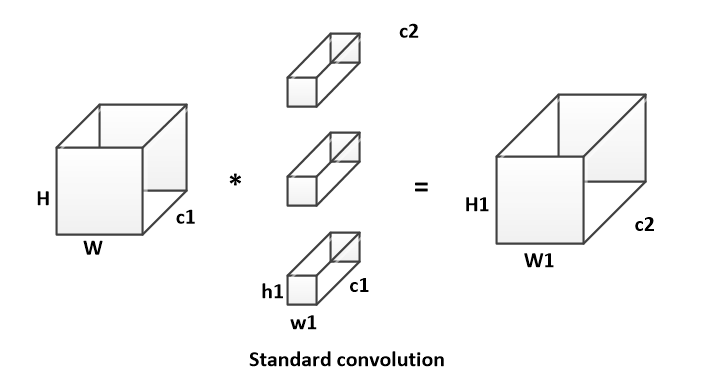
\includegraphics{./img/ch17/3.png} 传统卷积运算量为:\\
\[
A = H * W * h1 * w1 * c1 * c2
\] DW卷积的计算方式如下:\\
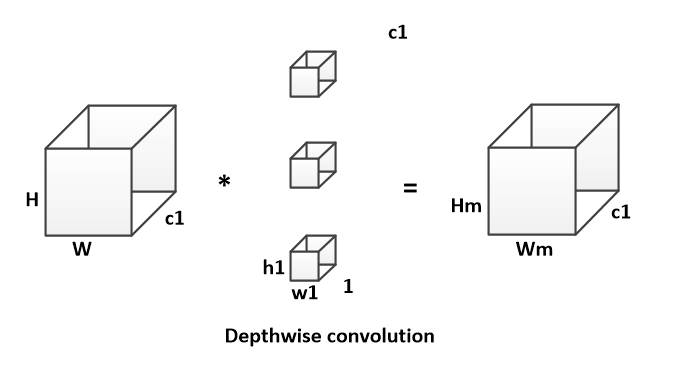
\includegraphics{./img/ch17/4.png} DW卷积运算量为: \[
B_DW = H * W * h1 * w1 * 1 * c1
\] PW卷积的计算方式如下: 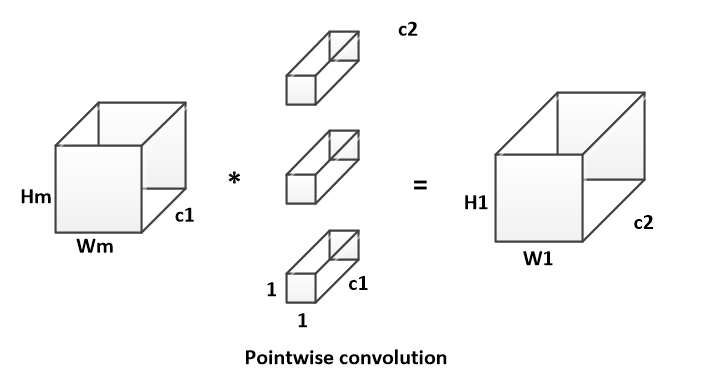
\includegraphics{./img/ch17/5.png}

\[
B_PW = H_m * W_m * 1 * 1 * c_1 * c_2
\] Depthwise separable convolution运算量为: \[
B = B_DW + B_PW
\] Depthwise separable convolution相对于传统卷积的运算量: \$\$
\dfrac{B}{A} =
\dfrac{ H * W * h_1 * w_1 * 1 * c_1 + H_m * W_m * 1 * 1 * c_1 * c_2}{H * W * h1 * w1 * c_1 * c_2}

= \dfrac{1}{c_2} + \dfrac{1}{h_1 * w_1} \$\$
由此可知,随着卷积通道数的增加,Depthwise separable
convolution的运算量相对于传统卷积更少。

\subsubsection{17.8.3
输入输出的channel相同时,MAC最小}\label{ux8f93ux5165ux8f93ux51faux7684channelux76f8ux540cux65f6macux6700ux5c0f}

\textbf{卷积层的输入和输出特征通道数相等时MAC最小,此时模型速度最快。}\\
假设feature map的大小为h*w,输入通道\(c_1\),输出通道\(c_2\)。\\
已知: \[
FLOPs = B = h * w * c1 * c2   
=> c1 * c2 = \dfrac{B}{h * w}   
\]

\[
MAC = h * w * (c1 + c2) + c1 * c2  
\]

\[
=> MAC \geq 2 * h * w \sqrt{\dfrac{B}{h * w}} + \dfrac{B}{h * w}
\]

根据均值不等式得到(c1-c2)\^{}2\textgreater{}=0,等式成立的条件是c1=c2,也就是输入特征通道数和输出特征通道数相等时,在给定FLOPs前提下,MAC达到取值的下界。

\subsubsection{17.8.4
减少组卷积的数量}\label{ux51cfux5c11ux7ec4ux5377ux79efux7684ux6570ux91cf}

\textbf{过多的group操作会增大MAC,从而使模型速度变慢}\\
由以上公式可知,group卷积想比与传统的卷积可以降低计算量,提高模型的效率;如果在相同的FLOPs时,group卷积为了满足FLOPs会是使用更多channels,可以提高模型的精度。但是随着channel数量的增加,也会增加MAC。\\
FLOPs: \[
B = \dfrac{h * w * c1 * c2}{g}
\] MAC: \[
MAC = h * w * (c1 + c2) + \dfrac{c1 * c2}{g}
\] 由MAC,FLOPs可知: \[
MAC = h * w * c1 + \dfrac{B*g}{c1} + \dfrac{B}{h * w}
\] 当FLOPs固定(B不变)时,g越大,MAC越大。

\subsubsection{17.8.5
减少网络碎片化程度(分支数量)}\label{ux51cfux5c11ux7f51ux7edcux788eux7247ux5316ux7a0bux5ea6ux5206ux652fux6570ux91cf}

\textbf{模型中分支数量越少,模型速度越快}\\
此结论主要是由实验结果所得。\\
以下为网络分支数和各分支包含的卷积数目对神经网络速度的影响。\\
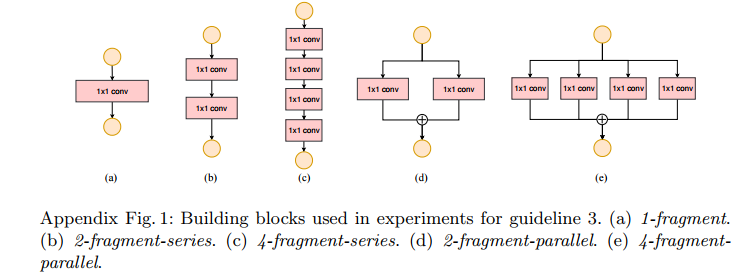
\includegraphics{./img/ch17/6.png}
实验中使用的基本网络结构,分别将它们重复10次,然后进行实验。实验结果如下:
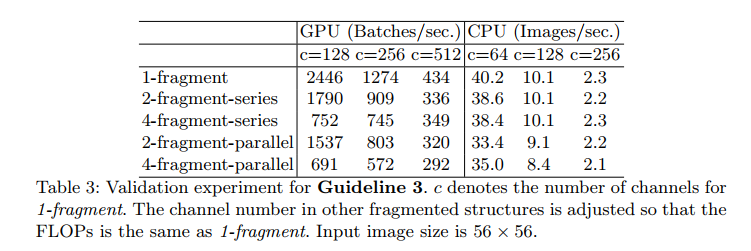
\includegraphics{./img/ch17/7.png}
由实验结果可知,随着网络分支数量的增加,神经网络的速度在降低。网络碎片化程度对GPU的影响效果明显,对CPU不明显,但是网络速度同样在降低。

\subsubsection{17.8.7
减少元素级操作}\label{ux51cfux5c11ux5143ux7d20ux7ea7ux64cdux4f5c}

\textbf{元素级操作所带来的时间消耗也不能忽视}\\
ReLU ,Tensor 相加,Bias相加的操作,分离卷积(depthwise
convolution)都定义为元素级操作。\\
FLOPs大多数是对于卷积计算而言的,因为元素级操作的FLOPs相对要低很多。但是过的元素级操作也会带来时间成本。ShuffleNet作者对ShuffleNet
v1和MobileNet
v2的几种层操作的时间消耗做了分析,发现元素级操作对于网络速度的影响也很大。
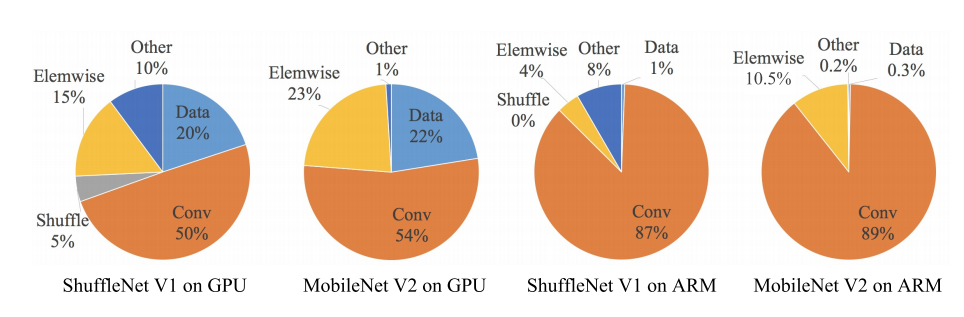
\includegraphics{./img/ch17/8.png}

\subsection{17.9
常用的轻量级网络有哪些?}\label{ux5e38ux7528ux7684ux8f7bux91cfux7ea7ux7f51ux7edcux6709ux54eaux4e9b}

\subsubsection{17.9.1 SequeezeNet}\label{sequeezenet}

SqueenzeNet出自F. N. Iandola, S.Han等人发表的论文《SqueezeNet:
AlexNet-level accuracy with 50x fewer parameters and \textless{} 0.5MB
model
size》,作者在保证精度不损失的同时,将原始AlexNet压缩至原来的510倍。\\
\#\#\#\# 1.1 设计思想 在网络结构设计方面主要采取以下三种方式: *
用1*1卷积核替换3*3卷积 *
理论上一个1*1卷积核的参数是一个3*3卷积核的1/9,可以将模型尺寸压缩9倍。 *
减小3*3卷积的输入通道数 *
根据上述公式,减少输入通道数不仅可以减少卷积的运算量,而且输入通道数与输出通道数相同时还可以减少MAC。
* 延迟降采样 *
分辨率越大的输入能够提供更多特征的信息,有利于网络的训练判断,延迟降采样可以提高网络精度。
\#\#\#\# 1.2 网络架构 SqueezeNet提出一种多分支结构------fire
model,其中是由Squeeze层和expand层构成。Squeeze层是由s1个1*1卷积组成,主要是通过1*1的卷积降低expand层的输入维度;expand层利用e1个1*1和e3个3*3卷积构成多分支结构提取输入特征,以此提高网络的精度(其中e1=e3=4*s1)。
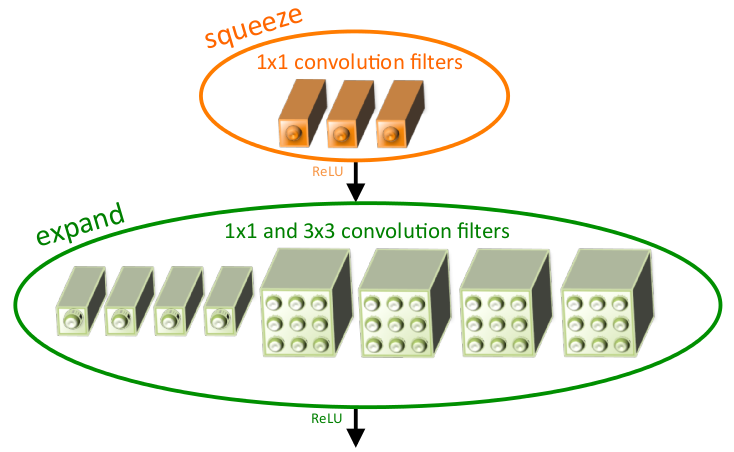
\includegraphics{./img/ch17/9.png} SqueezeNet整体网络结构如下图所示:
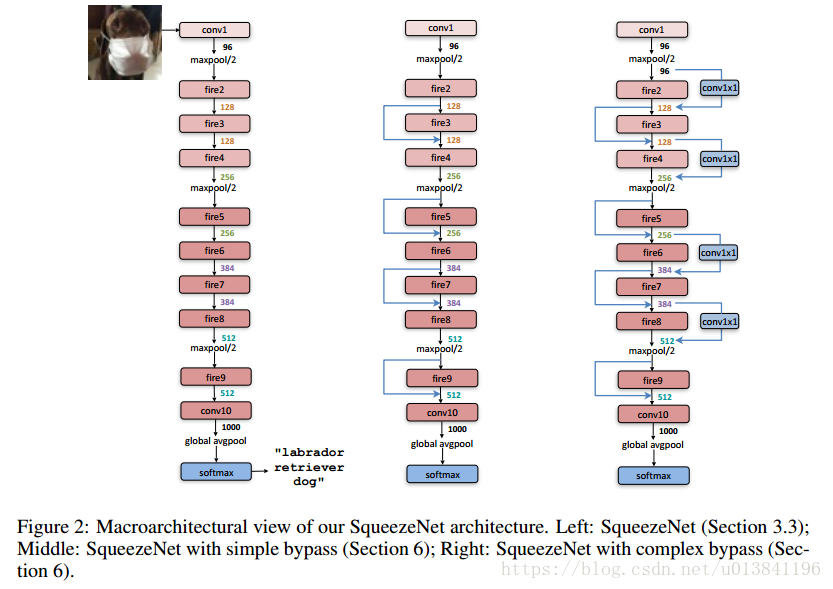
\includegraphics{./img/ch17/10.png}

\paragraph{1.3实验结果}\label{ux5b9eux9a8cux7ed3ux679c}

不同压缩方法在ImageNet上的对比实验结果
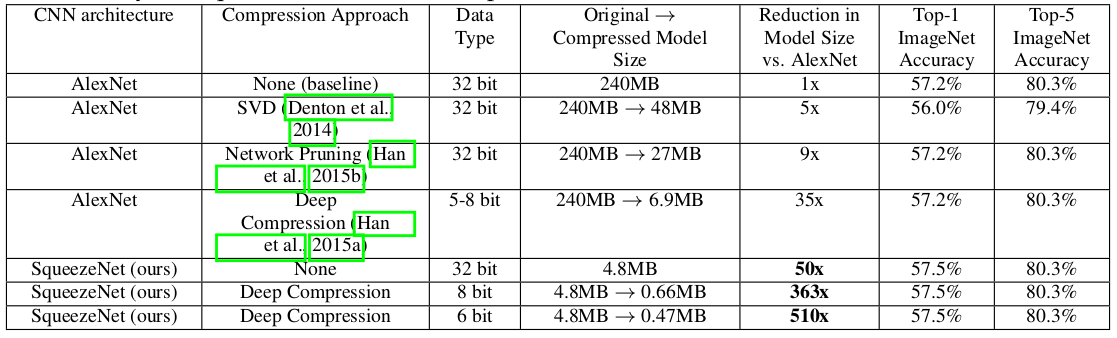
\includegraphics{./img/ch17/11.png}
由实验结果可知,SqueezeNet不仅保证了精度,而且将原始AlexNet从240M压缩至4.8M,压缩50倍,说明此轻量级网络设计是可行。

\subsubsection{17.9.2 MobileNet}\label{mobilenet}

MobileNet 是Google团队于CVPR-2017的论文《MobileNets: Efficient
Convolutional Neural Networks for Mobile Vision
Applications》中针对手机等嵌入式设备提出的一种轻量级的深层神经网络,该网络结构在VGG的基础上使用DW+PW的组合,在保证不损失太大精度的同时,降低模型参数量。
\#\#\#\# 2.1 设计思想 * 采用深度可分离卷积代替传统卷积 *
采用DW卷积在减少参数数量的同时提升运算速度。但是由于每个feature
map只被一个卷积核卷积,因此经过DW输出的feature
map不能只包含输入特征图的全部信息,而且特征之间的信息不能进行交流,导致``信息流通不畅''。
* 采用PW卷积实现通道特征信息交流,解决DW卷积导致``信息流通不畅''的问题。
* 使用stride=2的卷积替换pooling *
直接在卷积时利用stride=2完成了下采样,从而节省了需要再去用pooling再去进行一次下采样的时间,可以提升运算速度。同时,因为pooling之前需要一个stride=1的
conv,而与stride=2 conv的计算量想比要高近4倍(\textbf{个人理解})。
\#\#\#\# 2.2 网络架构 * DW conv和PW conv MobileNet的网络架构主要是由DW
conv和PW
conv组成,相比于传统卷积可以降低\(\dfrac{1}{N} + \dfrac{1}{Dk}​\)倍的计算量。\\
标准卷积与DW conv和PW conv如图所示:\\
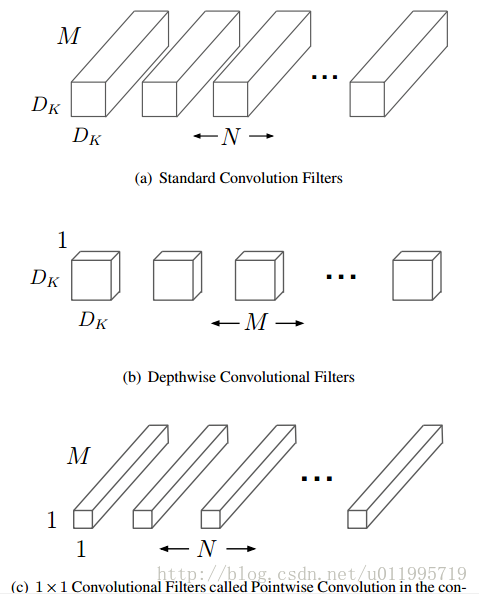
\includegraphics{./img/ch17/12.png} 深度可分离卷积与传统卷积运算量对比:
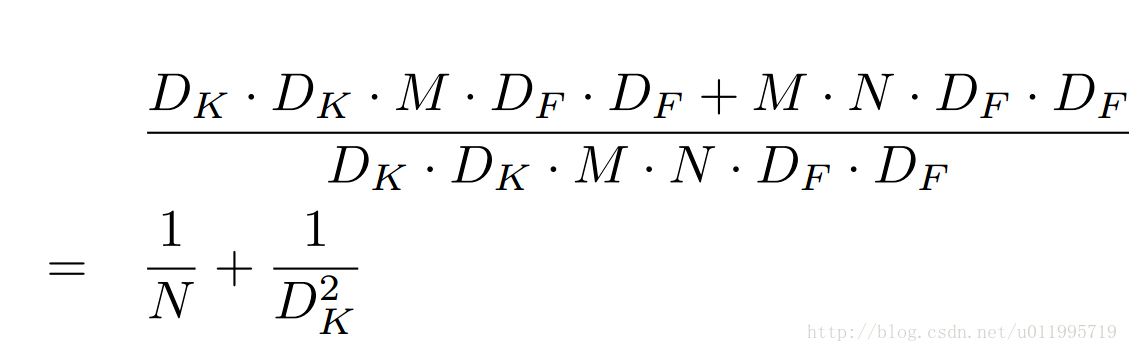
\includegraphics{./img/ch17/13.png} 网络结构:
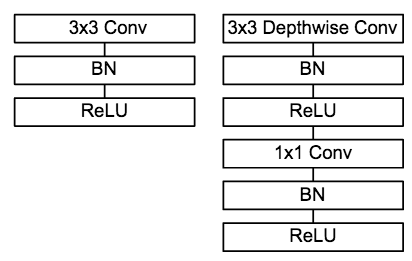
\includegraphics{./img/ch17/14.png}

\begin{itemize}
% \tightlist
\item
  MobileNets的架构 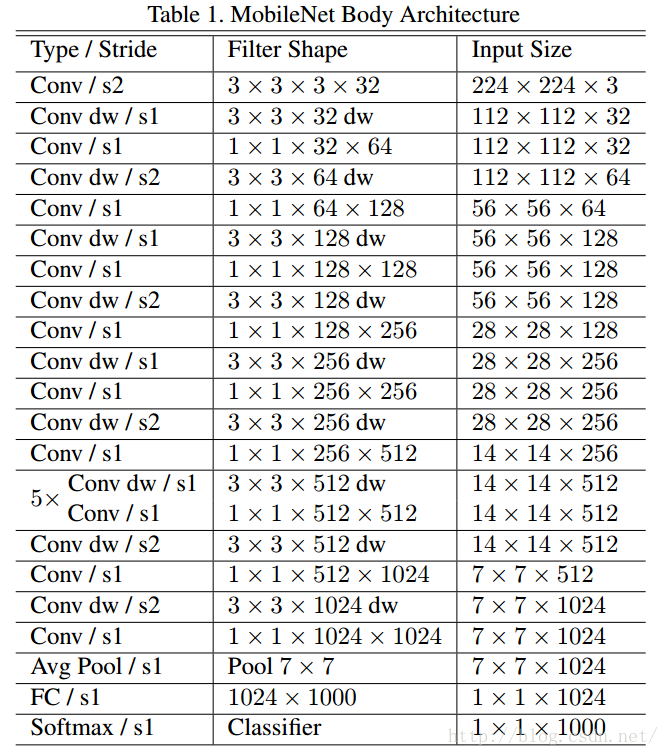
\includegraphics{./img/ch17/15.png}
\end{itemize}

\paragraph{2.3 实验结果}\label{ux5b9eux9a8cux7ed3ux679c-1}

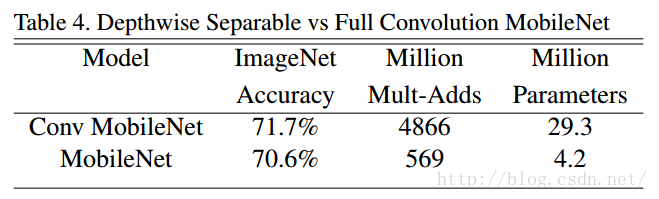
\includegraphics{./img/ch17/16.png}
由上表可知,使用相同的结构,深度可分离卷积虽然准确率降低1\%,但是参数量减少了6/7。

\subsubsection{17.9.3 MobileNet-v2}\label{mobilenet-v2}

MobileNet-V2是2018年1月公开在arXiv上论文《Inverted Residuals and Linear
Bottlenecks: Mobile Networks for Classification, Detection and
Segmentation》,是对MobileNet-V1的改进,同样是一个轻量化卷积神经网络。
\#\#\#\# 3.1 设计思想 * 采用Inverted residuals *
为了保证网络可以提取更多的特征,在residual block中第一个1*1
Conv和3\emph{3 DW Conv之前进行通道扩充 } Linear bottlenecks *
为了避免Relu对特征的破坏,在residual block的Eltwise sum之前的那个 1*1
Conv 不再采用Relu *
stride=2的conv不使用shot-cot,stride=1的conv使用shot-cut

\paragraph{3.2 网络架构}\label{ux7f51ux7edcux67b6ux6784}

\begin{itemize}
% \tightlist
\item
  Inverted residuals\\
  ResNet中Residuals block先经过1*1的Conv layer,把feature
  map的通道数降下来,再经过3*3 Conv layer,最后经过一个1*1 的Conv
  layer,将feature map
  通道数再``扩张''回去。即采用先压缩,后扩张的方式。而 inverted
  residuals采用先扩张,后压缩的方式。\\
  MobileNet采用DW conv提取特征,由于DW
  conv本身提取的特征数就少,再经过传统residuals
  block进行``压缩'',此时提取的特征数会更少,因此inverted
  residuals对其进行``扩张'',保证网络可以提取更多的特征。
  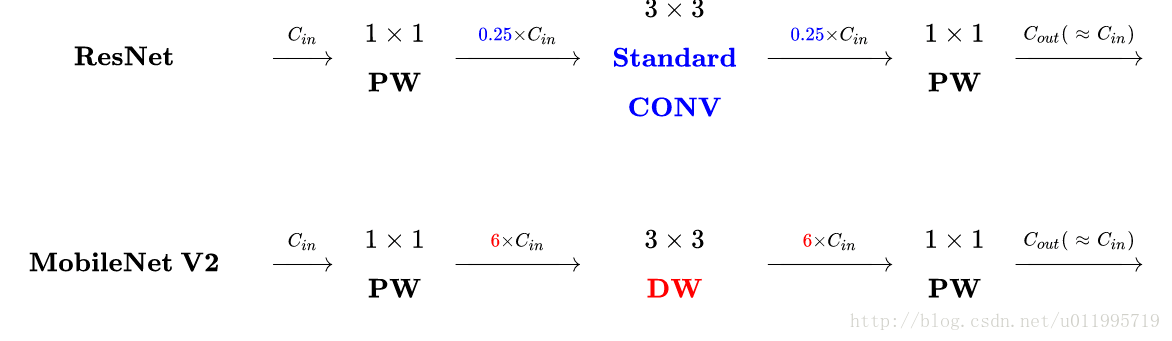
\includegraphics{./img/ch17/17.png}
\item
  Linear bottlenecks\\
  ReLu激活函数会破坏特征。ReLu对于负的输入,输出全为0,而本来DW
  conv特征通道已经被``压缩'',再经过ReLu的话,又会损失一部分特征。采用Linear,目的是防止Relu破坏特征。
  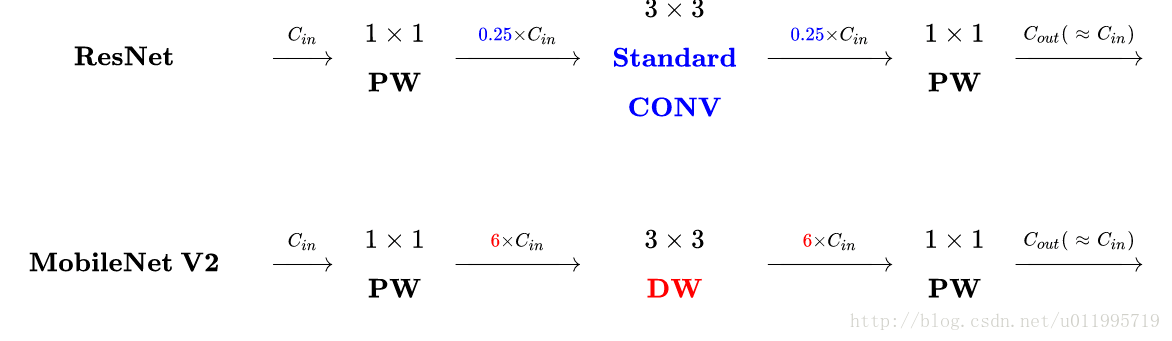
\includegraphics{./img/ch17/18.png}
\item
  shortcut\\
  stride=2的conv不使用shot-cot,stride=1的conv使用shot-cut
  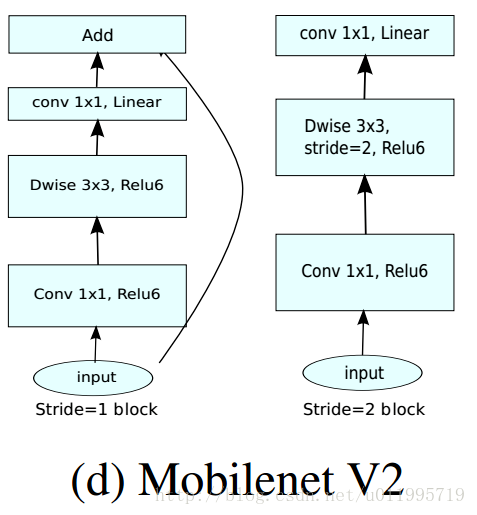
\includegraphics{./img/ch17/19.png}
\item
  网络架构\\
  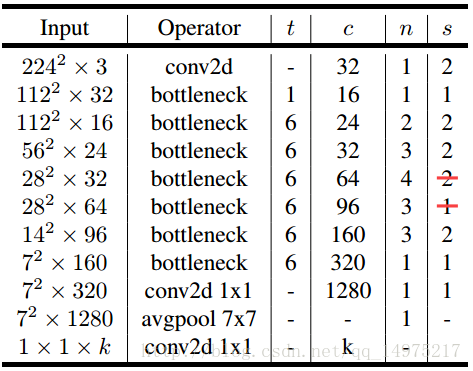
\includegraphics{./img/ch17/20.png}
\end{itemize}

\subsubsection{17.9.4 Xception}\label{xception}

Xception是Google提出的,arXiv 的V1 于2016年10月公开《Xception: Deep
Learning with Depthwise Separable Convolutions 》,Xception是对Inception
v3的另一种改进,主要是采用depthwise separable
convolution来替换原来Inception v3中的卷积操作。 \#\#\#\# 4.1设计思想 *
采用depthwise separable convolution来替换原来Inception v3中的卷积操作\\
与原版的Depth-wise convolution有两个不同之处: * 第一个:原版Depth-wise
convolution,先逐通道卷积,再1\emph{1卷积;
而Xception是反过来,先1*1卷积,再逐通道卷积; } 第二个:原版Depth-wise
convolution的两个卷积之间是不带激活函数的,而Xception在经过1*1卷积之后会带上一个Relu的非线性激活函数;

\paragraph{4.2网络架构}\label{ux7f51ux7edcux67b6ux6784-1}

feature
map在空间和通道上具有一定的相关性,通过Inception模块和非线性激活函数实现通道之间的解耦。增多3*3的卷积的分支的数量,使它与1*1的卷积的输出通道数相等,此时每个3*3的卷积只作用与一个通道的特征图上,作者称之为``极致的Inception(Extream
Inception)''模块,这就是Xception的基本模块。
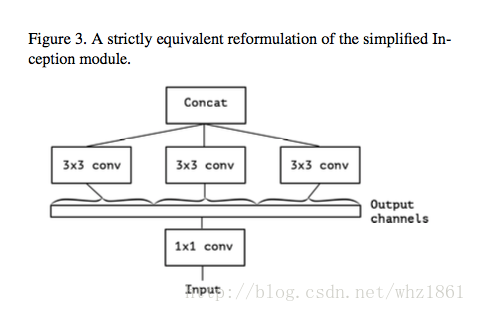
\includegraphics{./img/ch17/21.png}

\subsubsection{17.9.5 ShuffleNet-v1}\label{shufflenet-v1}

ShuffleNet
是Face++团队提出的,晚于MobileNet两个月在arXiv上公开《ShuffleNet: An
Extremely Efficient Convolutional Neural Network for Mobile Devices
》用于移动端前向部署的网络架构。ShuffleNet基于MobileNet的group思想,将卷积操作限制到特定的输入通道。而与之不同的是,ShuffleNet将输入的group进行打散,从而保证每个卷积核的感受野能够分散到不同group的输入中,增加了模型的学习能力。
\#\#\#\# 5.1 设计思想 * 采用group conv减少大量参数 * roup conv与DW
conv存在相同的``信息流通不畅''问题 * 采用channel shuffle解决上述问题 *
MobileNet中采用PW conv解决上述问题,SheffleNet中采用channel shuffle *
采用concat替换add操作 * avg pooling和DW conv(s=2)会减小feature
map的分辨率,采用concat增加通道数从而弥补分辨率减小而带来信息的损失

\paragraph{5.2 网络架构}\label{ux7f51ux7edcux67b6ux6784-2}

MobileNet中1*1卷积的操作占据了约95\%的计算量,所以作者将1*1也更改为group卷积,使得相比MobileNet的计算量大大减少。
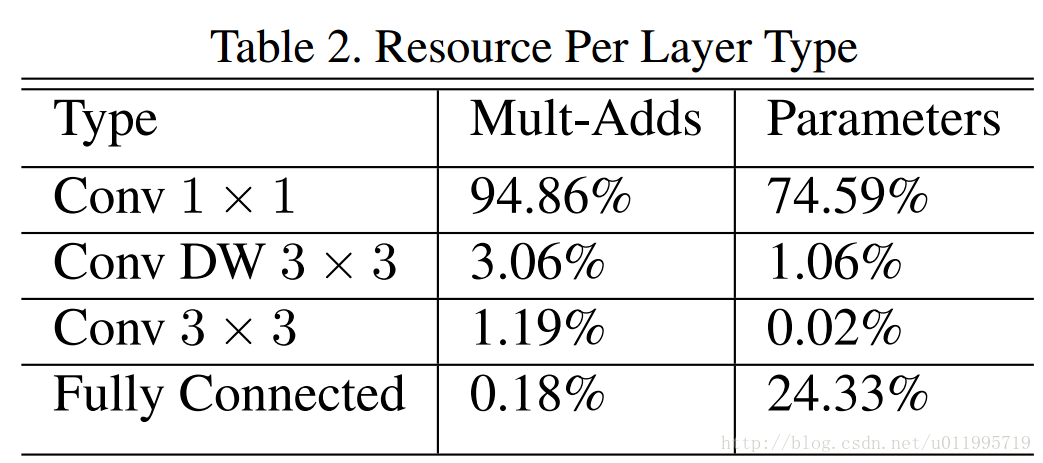
\includegraphics{./img/ch17/22.png}
group卷积与DW存在同样使``通道信息交流不畅''的问题,MobileNet中采用PW
conv解决上述问题,SheffleNet中采用channel shuffle。\\
ShuffleNet的shuffle操作如图所示 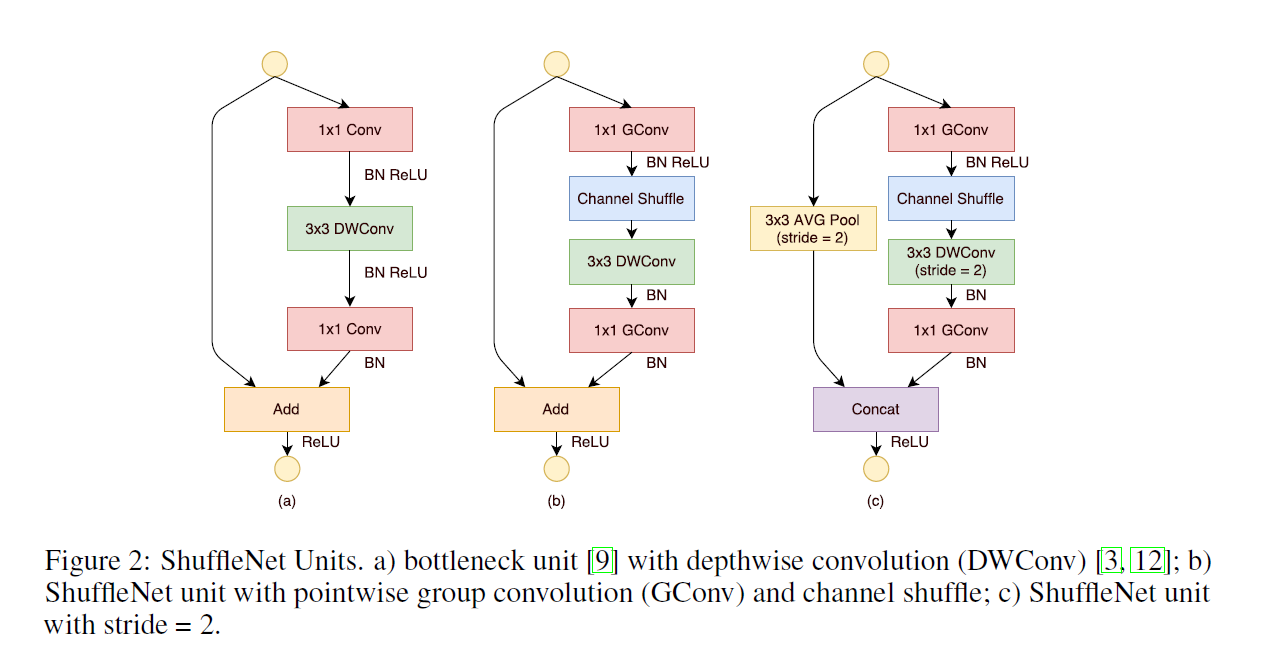
\includegraphics{./img/ch17/24.png} avg
pooling和DW conv(s=2)会减小feature
map的分辨率,采用concat增加通道数从而弥补分辨率减小而带来信息的损失;实验表明:多多使用通道(提升通道的使用率),有助于提高小模型的准确率。
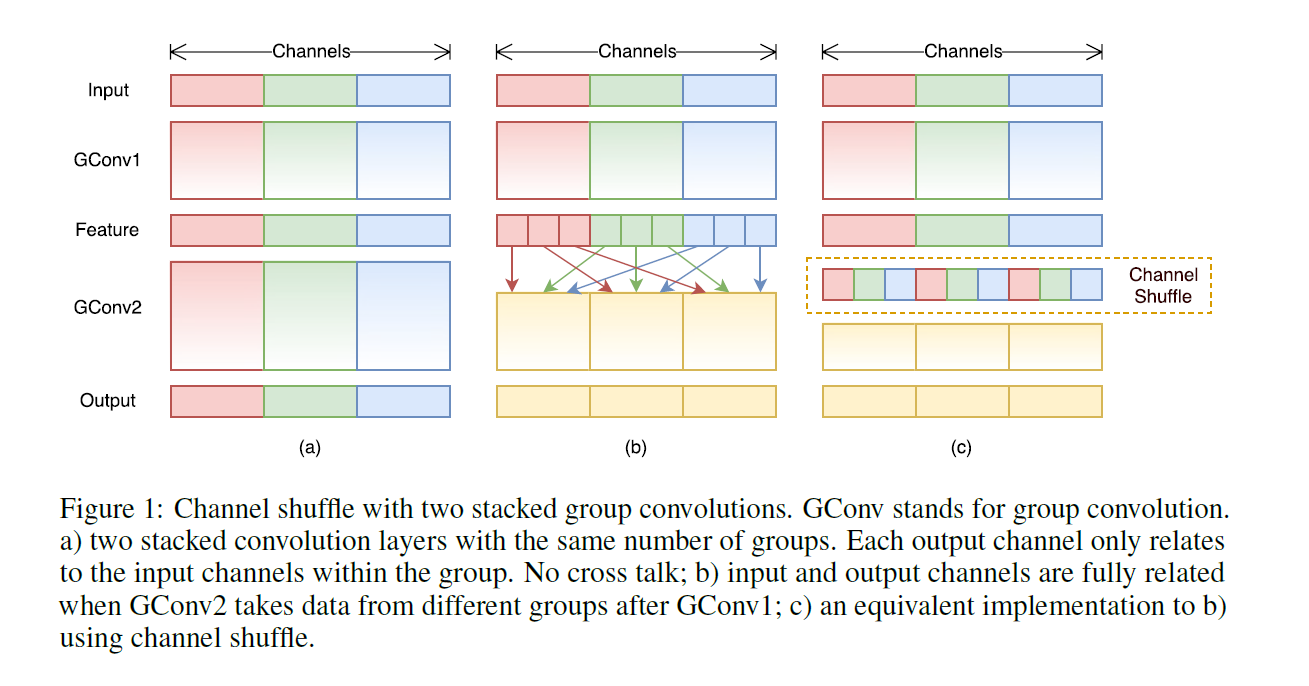
\includegraphics{./img/ch17/23.png} 网络结构:\\
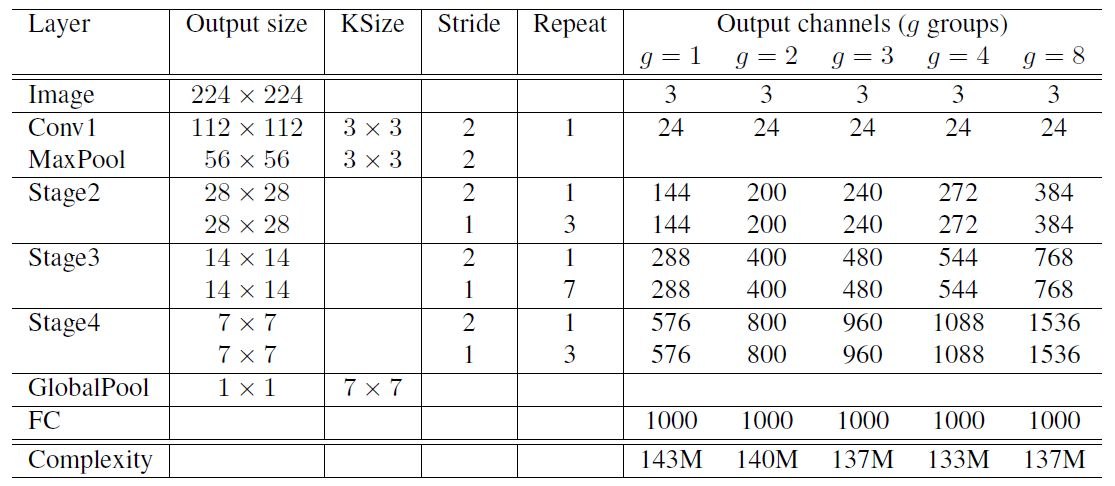
\includegraphics{./img/ch17/25.png}

\subsubsection{17.9.6 ShuffleNet-v2}\label{shufflenet-v2}

huffleNet-v2 是Face++团队提出的《ShuffleNet V2: Practical Guidelines for
Ecient CNN Architecture
Design》,旨在设计一个轻量级但是保证精度、速度的深度网络。 \#\#\#\# 6.1
设计思想 * 文中提出影响神经网络速度的4个因素: * a.
FLOPs(FLOPs就是网络执行了多少multiply-adds操作) * b. MAC(内存访问成本) *
c. 并行度(如果网络并行度高,速度明显提升) * d. 计算平台(GPU,ARM) *
ShuffleNet-v2 提出了4点网络结构设计策略: *
G1.输入输出的channel相同时,MAC最小 * G2.过度的组卷积会增加MAC *
G3.网络碎片化会降低并行度 * G4.元素级运算不可忽视

\paragraph{6.2 网络结构}\label{ux7f51ux7edcux7ed3ux6784}

depthwise convolution 和 瓶颈结构增加了 MAC,用了太多的
group,跨层连接中的 element-wise Add 操作也是可以优化的点。所以在
shuffleNet V2 中增加了几种新特性。\\
所谓的 channel split
其实就是将通道数一分为2,化成两分支来代替原先的分组卷积结构(G2),并且每个分支中的卷积层都是保持输入输出通道数相同(G1),其中一个分支不采取任何操作减少基本单元数(G3),最后使用了
concat 代替原来的 elementy-wise add,并且后面不加 ReLU
直接(G4),再加入channle shuffle 来增加通道之间的信息交流。
对于下采样层,在这一层中对通道数进行翻倍。
在网络结构的最后,即平均值池化层前加入一层 1x1
的卷积层来进一步的混合特征。 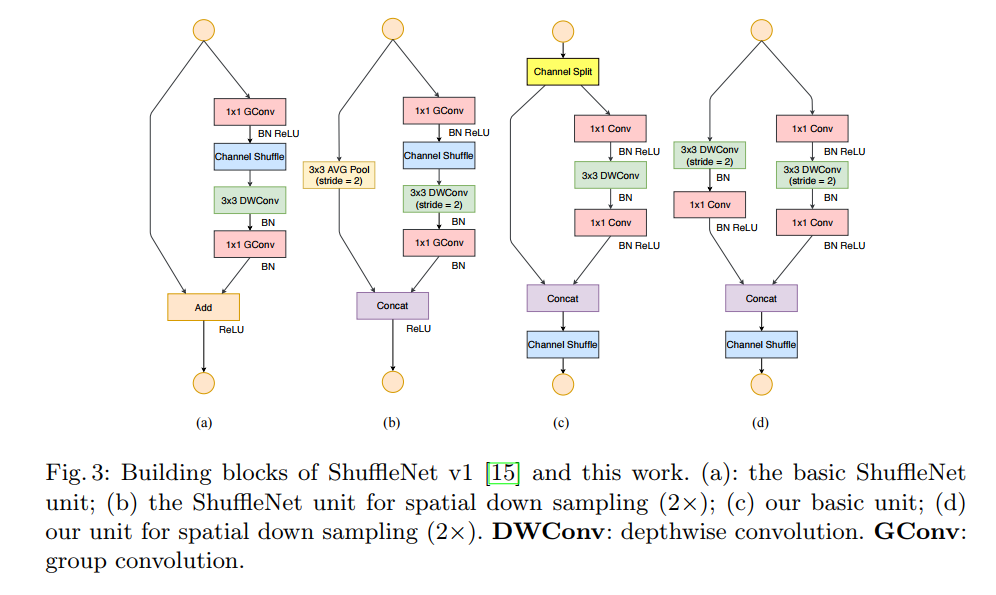
\includegraphics{./img/ch17/26.png}
网络结构\\
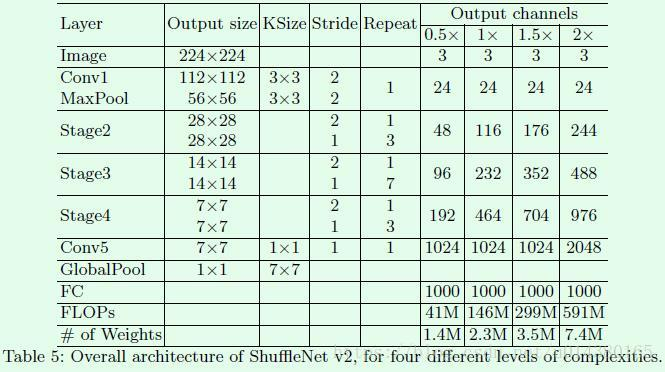
\includegraphics{./img/ch17/27.png}

\paragraph{6.4
ShuffleNet-v2具有高精度的原因}\label{shufflenet-v2ux5177ux6709ux9ad8ux7cbeux5ea6ux7684ux539fux56e0}

\begin{itemize}
% \tightlist
\item
  由于高效,可以增加更多的channel,增加网络容量
\item
  采用split使得一部分特征直接与下面的block相连,特征复用(DenseNet)
\end{itemize}

\subsection{17.10
现有移动端开源框架及其特点}\label{ux73b0ux6709ux79fbux52a8ux7aefux5f00ux6e90ux6846ux67b6ux53caux5176ux7279ux70b9}

\subsubsection{17.10.1 NCNN}\label{ncnn}

1、开源时间:2017年7月   

2、开源用户:腾讯优图    

3、GitHub地址:https://github.com/Tencent/ncnn   

4、特点:

\begin{itemize}
% \tightlist
\item
  1)NCNN考虑了手机端的硬件和系统差异以及调用方式,架构设计以手机端运行为主要原则。
\item
  2)无第三方依赖,跨平台,手机端 CPU
  的速度快于目前所有已知的开源框架(以开源时间为参照对象)。
\item
  3)基于
  ncnn,开发者能够将深度学习算法轻松移植到手机端高效执行,开发出人工智能
  APP。
\end{itemize}

5、功能:

\begin{itemize}
% \tightlist
\item
  1、NCNN支持卷积神经网络、多分支多输入的复杂网络结构,如vgg、googlenet、resnet、squeezenet
  等。
\item
  2、NCNN无需依赖任何第三方库。\\
\item
  3、NCNN全部使用C/C++实现,以及跨平台的cmake编译系统,可轻松移植到其他系统和设备上。\\
\item
  4、汇编级优化,计算速度极快。使用ARM
  NEON指令集实现卷积层,全连接层,池化层等大部分 CNN 关键层。
\item
  5、精细的数据结构设计,没有采用需消耗大量内存的通常框架------im2col +
  矩阵乘法,使得内存占用极低。\\
\item
  6、支持多核并行计算,优化CPU调度。\\
\item
  7、整体库体积小于500K,可精简到小于300K。\\
\item
  8、可扩展的模型设计,支持8bit 量化和半精度浮点存储。\\
\item
  9、支持直接内存引用加载网络模型。\\
\item
  10、可注册自定义层实现并扩展。
\end{itemize}

6、NCNN在Android端部署示例

\begin{itemize}
% \tightlist
\item
  1)选择合适的Android Studio版本并安装。
\item
  2)根据需求选择NDK版本并安装。
\item
  3)在Android Studio上配置NDK的环境变量。
\item
  4)根据自己需要编译NCNN sdk
\end{itemize}

\begin{verbatim}
mkdir build-android cd build-android cmake -DCMAKE_TOOLCHAIN_FILE=$ANDROID_NDK/build/cmake/android.toolchain.cmake \ -DANDROID_ABI="armeabi-v7a" -DANDROID_ARM_NEON=ON \ -DANDROID_PLATFORM=android-14 .. make make install
\end{verbatim}

​ 安装完成之后,install下有include和lib两个文件夹。

​ 备注:

\begin{verbatim}
ANDROID_ABI 是架构名字,"armeabi-v7a" 支持绝大部分手机硬件 
ANDROID_ARM_NEON 是否使用 NEON 指令集,设为 ON 支持绝大部分手机硬件 
ANDROID_PLATFORM 指定最低系统版本,"android-14" 就是 android-4.0
\end{verbatim}

\begin{itemize}
% \tightlist
\item
  5)进行NDK开发。
\end{itemize}

\begin{verbatim}
1)assets文件夹下放置你的bin和param文件。
2)jni文件夹下放置你的cpp和mk文件。
3)修改你的app gradle文件。
4)配置Android.mk和Application.mk文件。
5)进行java接口的编写。
6)读取拷贝bin和param文件(有些则是pb文件,根据实际情况)。
7)进行模型的初始化和执行预测等操作。
8)build。
9)cd到src/main/jni目录下,执行ndk-build,生成.so文件。
10)接着就可写自己的操作处理需求。
\end{verbatim}

\subsubsection{17.10.2 QNNPACK}\label{qnnpack}

全称:Quantized Neural Network PACKage(量化神经网络包)   

1、开源时间:2018年10月   

2、开源用户:Facebook    

3、GitHub地址:https://github.com/pytorch/QNNPACK    

4、特点:   

​ 1)低密度卷积优化函数库;   

  2)可在手机上实时运行Mask R-CNN 和 DensePose;

​ 3) 能在性能受限的移动设备中用 100ms 以内的时间实施图像分类;   

5、QNNPACK 如何提高效率?

1)\textbf{QNNPACK 使用与安卓神经网络 API 兼容的线性量化方案}

QNNPACK
的输入矩阵来自低精度、移动专用的计算机视觉模型。其它库在计算A和B矩阵相乘时,重新打包
A 和 B
矩阵以更好地利用缓存层次结构,希望在大量计算中分摊打包开销,QNNPACK
删除所有计算非必需的内存转换,针对
A和B矩阵相乘适用于一级缓存的情况进行了优化。

\begin{figure}
\centering
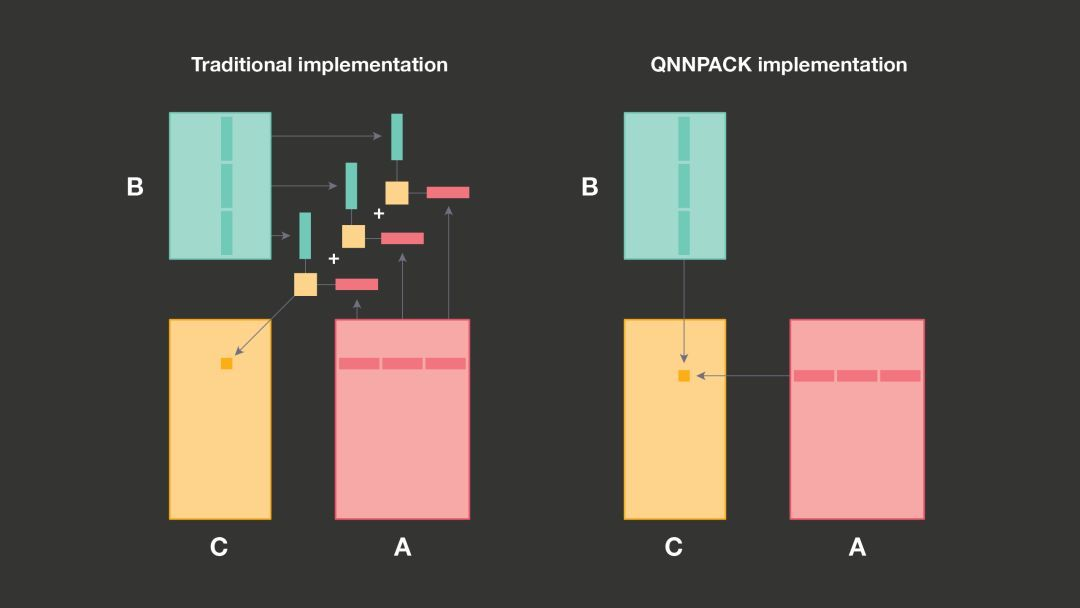
\includegraphics{./img/ch17/QNNPACK1.jpeg}
\caption{}
\end{figure}

​
1)优化了L1缓存计算,不需要输出中间结果,直接输出最终结果,节省内存带宽和缓存占用。

具体分析:

\begin{itemize}
% \tightlist
\item
  常规实现:在量化矩阵-矩阵乘法中,8位整数的乘积通常会被累加至 32
  位的中间结果中,随后重新量化以产生 8
  位的输出。遇到大矩阵尺寸时,比如有时K太大,A和B的面板无法直接转入缓存,此时,需利用缓存层次结构,借助GEMM将A和B的面板沿着K维分割成固定大小的子面板,以便于每个子面板都能适应L1缓存,随后为每个子面板调用微内核。这一缓存优化需要
  PDOT 为内核输出 32 位中间结果,最终将它们相加并重新量化为 8 位整数。
\item
  优化实现:由于 ONNPACK 对于面板 A 和 B 总是适应 L1
  缓存的移动神经网络进行了优化,因此它在调用微内核时处理整个 A 和 B
  的面板。而由于无需在微内核之外积累 32 位的中间结果,QNNPACK 会将 32
  位的中间结果整合进微内核中并写出 8 位值,这节省了内存带宽和缓存占用。
\end{itemize}

\begin{figure}
\centering
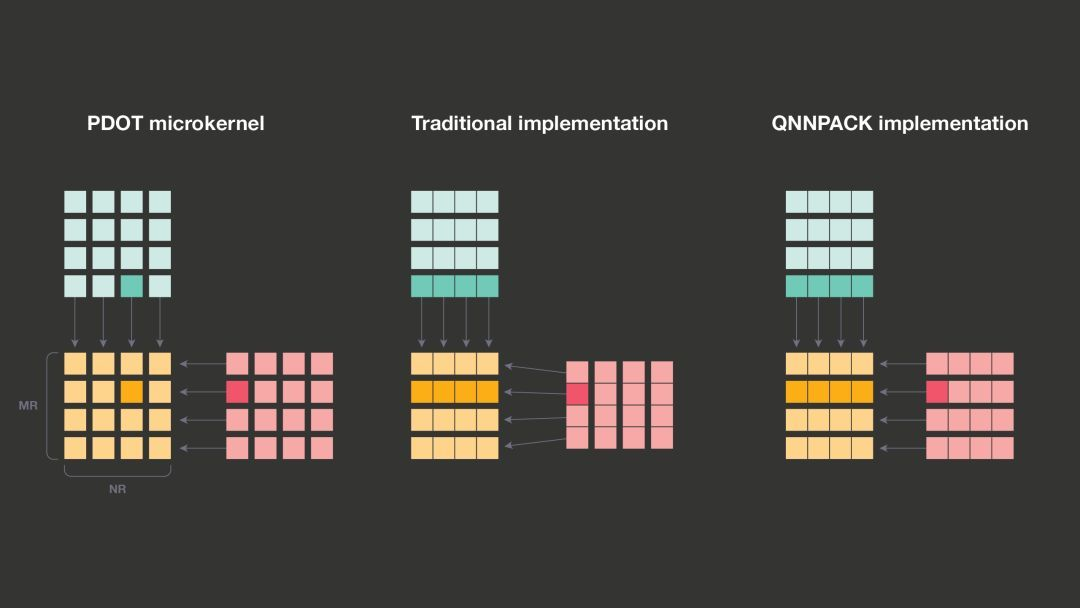
\includegraphics{./img/ch17/QNNPACK2.jpeg}
\caption{}
\end{figure}

​ 2)取消了矩阵 A 的重新打包。

\begin{itemize}
\item
  常规实现:

\begin{verbatim}
矩阵 B 包含静态权重,可以一次性转换成任何内存布局,但矩阵  A 包含卷积输入,每次推理运行都会改变。因此,重新打包矩阵 A 在每次运行时都会产生开销。尽管存在开销,传统的 GEMM实现还是出于以下两个原因对矩阵 A 进行重新打包:

a 缓存关联性及微内核效率受限。如果不重新打包,微内核将不得不读取被潜在的大跨距隔开的几行A。如果这个跨距恰好是 2 的许多次幂的倍数,面板中不同行 A  的元素可能会落入同一缓存集中。如果冲突的行数超过了缓存关联性,它们就会相互驱逐,性能也会大幅下降。

b 打包对微内核效率的影响与当前所有移动处理器支持的  SIMD  向量指令的使用密切相关。这些指令加载、存储或者计算小型的固定大小元素向量,而不是单个标量(scalar)。在矩阵相乘中,充分利用向量指令达到高性能很重要。在传统的  GEMM 实现中,微内核把 MR 元素重新打包到向量暂存器里的 MR 线路中。
\end{verbatim}
\item
  优化实现:

\begin{verbatim}
a 当面板适配一级缓存时,不会存在缓存关联性及微内核效率受限的问题。

b 在 QNNPACK 实现中,MR  元素在存储中不是连续的,微内核需要把它们加载到不同的向量暂存器中。越来越大的暂存器压力迫使 QNNPACK 使用较小的 MRxNR  拼贴,但实际上这种差异很小,而且可以通过消除打包开销来补偿。例如,在 32 位 ARM 架构上,QNNPACK 使用 4×8 微内核,其中  57% 的向量指令是乘-加;另一方面,gemmlowp 库使用效率稍高的 4×12 微内核,其中 60% 的向量指令是乘-加。微内核加载 A  的多个行,乘以 B 的满列,结果相加,然后完成再量化并记下量化和。A 和 B 的元素被量化为 8 位整数,但乘积结果相加到 32 位。大部分  ARM 和 ARM64 处理器没有直接完成这一运算的指令,所以它必须分解为多个支持运算。QNNPACK  提供微内核的两个版本,其不同之处在于用于乘以 8 位值并将它们累加到 32 位的指令序列。
\end{verbatim}
\end{itemize}

2)\textbf{从矩阵相乘到卷积}

\begin{figure}
\centering
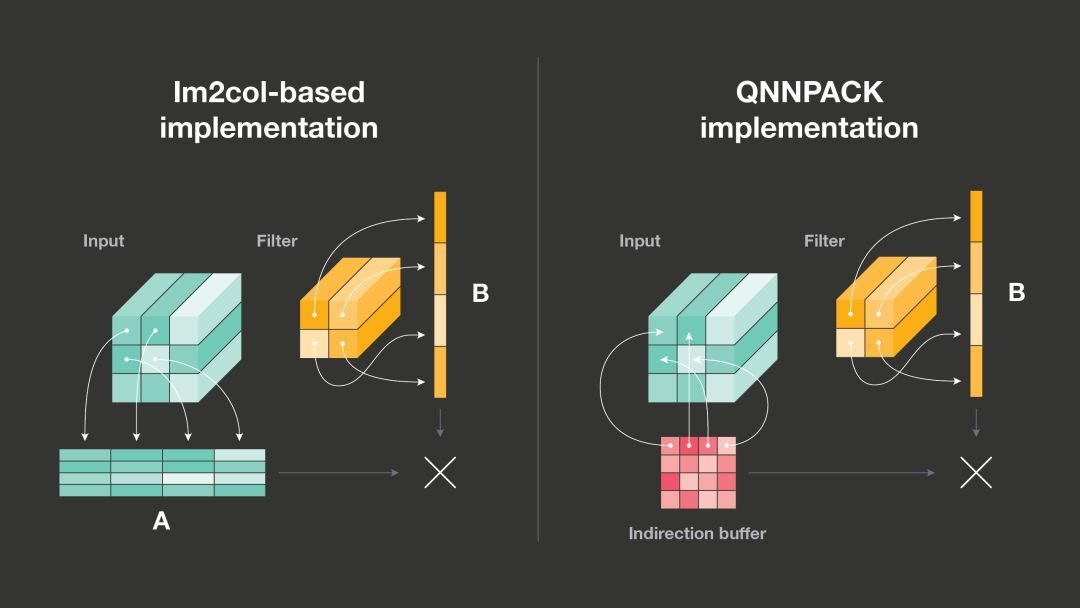
\includegraphics{./img/ch17/QNNPACK3.jpeg}
\caption{}
\end{figure}

​ 传统实现:

​ 简单的 1×1 卷积可直接映射到矩阵相乘

​ 但对于具备较大卷积核、padding
或子采样(步幅)的卷积而言则并非如此。但是,这些较复杂的卷积能够通过记忆变换
im2col 映射到矩阵相乘。对于每个输出像素,im2col
复制输入图像的图像块并将其计算为 2D 矩阵。由于每个输出像素都受 KHxKWxC
输入像素值的影响(KH 和 KW 分别指卷积核的高度和宽度,C
指输入图像中的通道数),因此该矩阵的大小是输入图像的 KHxKW 倍,im2col
给内存占用和性能都带来了一定的开销。和 Caffe
一样,大部分深度学习框架转而使用基于 im2col
的实现,利用现有的高度优化矩阵相乘库来执行卷积操作。

​ 优化实现:

​ Facebook 研究者在 QNNPACK 中实现了一种更高效的算法。

\begin{itemize}
% \tightlist
\item
  他们没有变换卷积输入使其适应矩阵相乘的实现,而是调整 PDOT
  微内核的实现,在运行中执行 im2col
  变换。这样就无需将输入张量的实际输入复制到 im2col
  缓存,而是使用输入像素行的指针设置 indirection
  buffer,输入像素与每个输出像素的计算有关。
\item
  研究者还修改了矩阵相乘微内核,以便从 indirection buffer
  加载虚构矩阵(imaginary matrix)A 的行指针,indirection buffer 通常比
  im2col buffer 小得多。
\item
  此外,如果两次推断运行的输入张量存储位置不变,则 indirection buffer
  还可使用输入张量行的指针进行初始化,然后在多次推断运行中重新使用。研究者观察到具备
  indirection buffer 的微内核不仅消除了 im2col
  变换的开销,其性能也比矩阵相乘微内核略好(可能由于输入行在计算不同输出像素时被重用)。
\end{itemize}

3)\textbf{深度卷积}

\begin{figure}
\centering
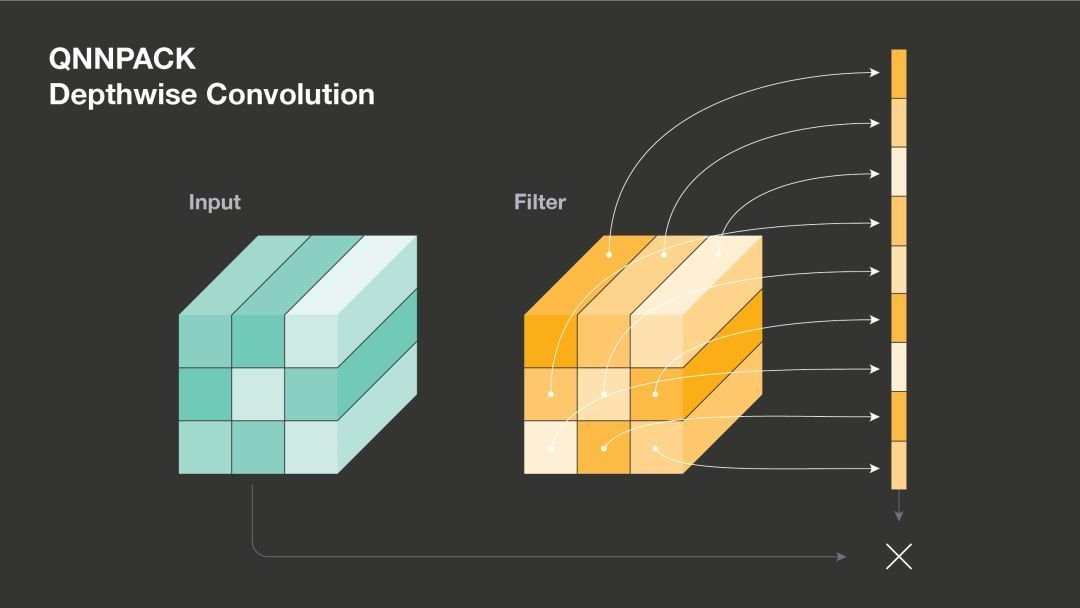
\includegraphics{./img/ch17/QNNPACK4.jpeg}
\caption{}
\end{figure}

分组卷积(grouped
convolution)将输入和输出通道分割成多组,然后对每个组进行分别处理。在有限条件下,当组数等于通道数时,该卷积就是深度卷积,常用于当前的神经网络架构中。深度卷积对每个通道分别执行空间滤波,展示了与正常卷积非常不同的计算模式。因此,通常要向深度卷积提供单独实现,QNNPACK
包括一个高度优化版本 3×3 深度卷积。

深度卷积的传统实现是每次都在卷积核元素上迭代,然后将一个卷积核行和一个输入行的结果累加到输出行。对于一个
3×3 的深度卷积,此类实现将把每个输出行更新 9 次。在 QNNPACK
中,研究者计算所有 3×3 卷积核行和 3×3
输入行的结果,一次性累加到输出行,然后再处理下个输出行。

QNNPACK
实现高性能的关键因素在于完美利用通用暂存器(GPR)来展开卷积核元素上的循环,同时避免在
hot loop 中重新加载地址寄存器。32-bit ARM 架构将实现限制在 14 个 GPR。在
3×3 深度卷积中,需要读取 9 个输入行和 9
个卷积核行。这意味着如果想完全展开循环必须存储 18
个地址。然而,实践中推断时卷积核不会发生变化。因此 Facebook
研究者使用之前在 CxKHxKW 中的滤波器,将它们封装进
{[}C/8{]}xKWxKHx8,这样就可以仅使用具备地址增量(address
increment)的一个 GPR 访问所有滤波器。(研究者使用数字 8
的原因在于,在一个命令中加载 8 个元素然后减去零,在 128-bit NEON
暂存器中生成 8 个 16-bit 值。)然后使用 9
个输入行指针,指针将滤波器重新装进 10 个
GPR,完全展开滤波器元素上的循环。64-bit ARM 架构相比 32-bit 架构,GPR
的数量翻了一倍。QNNPACK 利用额外的 ARM64 GPR,一次性存储 3×5
输入行的指针,并计算 3 个输出行。

7、性能优势:

​ 测试结果显示出 QNNPACK 在端到端基准上的性能优势。在量化当前最优
MobileNetV2 架构上,基于QNNPACK 的 Caffe2 算子的速度大约是 TensorFlow
Lite 速度的 2 倍,在多种手机上都是如此。除了 QNNPACK 之外,Facebook
还开源了 Caffe2 quantized MobileNet v2 模型,其 top-1 准确率比相应的
TensorFlow 模型高出 1.3\%。

\textbf{MobileNetV1}

MobileNetV1 架构在使用深度卷积(depthwise
convolution)使模型更适合移动设备方面具备开创性。MobileNetV1
包括几乎整个 1×1 卷积和 3×3 卷积。Facebook 研究者将量化 MobileNetV1
模型从 TensorFlow Lite 转换而来,并在 TensorFlow Lite 和 QNNPACK 的
32-bit ARM 设备上对 MobileNetV1 进行基准测试。二者运行时均使用 4
线程,研究者观察到 QNNPACK 的运行速度几何平均值是 TensorFlow Lite 的 1.8
倍。

\begin{figure}
\centering
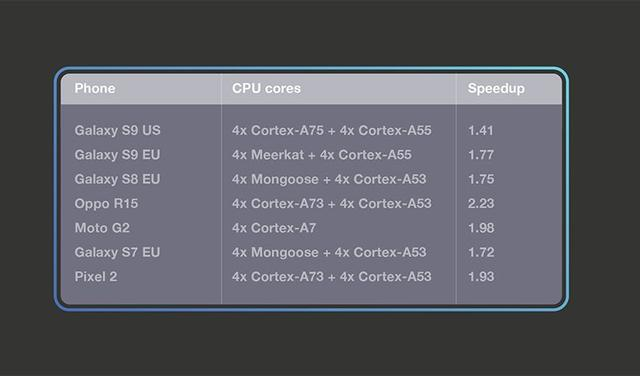
\includegraphics{./img/ch17/mv1.jpg}
\caption{}
\end{figure}

\textbf{MobileNetV2}

作为移动视觉任务的当前最优架构之一,MobileNetV2
引入了瓶颈构造块和瓶颈之间的捷径连接。研究者在 MobileNetV2
分类模型的量化版上对比基于 QNNPACK 的 Caffe2 算子和 TensorFlow Lite
实现。使用的量化 Caffe2 MobileNetV2 模型已开源,量化 TensorFlow Lite
模型来自官方库:https://github.com/tensorflow/tensorflow/blob/master/tensorflow/contrib/lite/g3doc/models.md。下表展示了二者在常用测试集上的
top1 准确率:

\begin{figure}
\centering
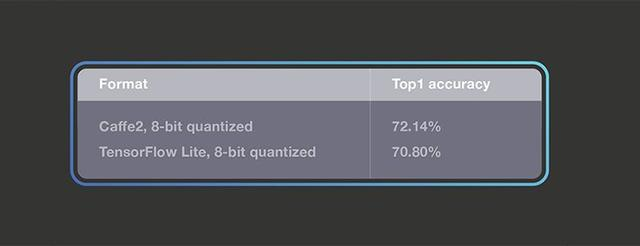
\includegraphics{./img/ch17/mv2.jpg}
\caption{}
\end{figure}

​ Facebook 研究者利用这些模型建立了 Facebook AI
性能评估平台(https://github.com/facebook/FAI-PEP)的基准,该基准基于
32-bit ARM 环境的大量手机设备。对于 TensorFlow Lite
线程设置,研究者尝试了一到四个线程,并报告了最快速的结果。结果显示
TensorFlow Lite 使用四线程的性能最优,因此后续研究中使用四线程来对比
TensorFlow Lite 和
QNNPACK。下表展示了结果,以及在典型智能手机和高端机上,基于 QNNPACK
的算子速度比 TensorFlow Lite 快得多。

\begin{figure}
\centering
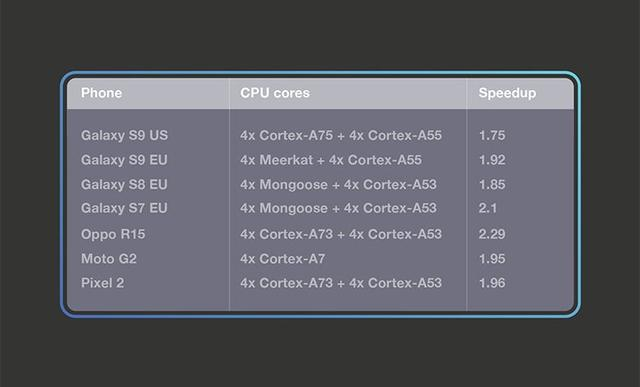
\includegraphics{./img/ch17/mv3.jpg}
\caption{}
\end{figure}

Facebook开源高性能内核库QNNPACK
https://baijiahao.baidu.com/s?id=1615725346726413945\&wfr=spider\&for=pc
http://www.sohu.com/a/272158070\_610300

支持移动端深度学习的几种开源框架
https://blog.csdn.net/zchang81/article/details/74280019

\subsubsection{17.10.3 Prestissimo}\label{prestissimo}

1、开源时间:2017年11月   

2、开源用户:九言科技    

3、GitHub地址:https://github.com/in66-dev/In-Prestissimo  

4、功能特点: 

\textbf{基础功能}

\begin{itemize}
% \tightlist
\item
  支持卷积神经网络,支持多输入和多分支结构
\item
  精炼简洁的API设计,使用方便
\item
  提供调试接口,支持打印各个层的数据以及耗时
\item
  不依赖任何第三方计算框架,整体库体积 500K 左右(32位 约400k,64位
  约600k)
\item
  纯 C++ 实现,跨平台,支持 android 和 ios
\item
  模型为纯二进制文件,不暴露开发者设计的网络结构
\end{itemize}

\textbf{极快的速度}

\begin{itemize}
% \tightlist
\item
  大到框架设计,小到汇编书写上全方位的优化,iphone7 上跑 SqueezeNet 仅需
  26ms(单线程)
\item
  支持浮点(float)和整型(int)两种运算模式,float模式精度与caffe相同,int模式运算速度快,大部分网络用int的精度便已经足够
\item
  以巧妙的内存布局提升cpu的cache命中率,在中低端机型上性能依然强劲
\item
  针对 float-arm32, float-arm64, int-arm32, int-arm64
  四个分支均做了细致的优化,保证arm32位和arm64位版本都有非常好的性能
\end{itemize}

\textbf{SqueezeNet-v1.1 测试结果}

\textbf{Note}: 手机测试性能存在一定的抖动,连续多次运算取平均时间

\textbf{Note}: 像华为mate8, mate9,Google nexus 6
虽然是64位的CPU,但测试用的是 32位的库,因此cpu架构依然写 arm-v7a

\begin{longtable}[]{ ccccccc }
\toprule
CPU架构 & 机型 & CPU & ncnn(4线程) & mdl & Prestissimo\_float(单线程)
& Prestissimo\_int(单线程)\tabularnewline
\midrule
\endhead
arm-v7a & 小米2 & 高通APQ8064 1.5GHz & 185 ms & 370 ms & 184 ms & 115
ms\tabularnewline
arm-v7a & 小米2s & 四核 骁龙APQ8064 Pro 1.7GHz & 166 ms & - & 136 ms &
96 ms\tabularnewline
arm-v7a & 红米Note 4x & 骁龙625 四核2.0GHz & 124 ms & 306 ms & 202 ms &
110 ms\tabularnewline
arm-v7a & Google Nexus 6 & 骁龙805 四核 2.7GHz & 84 ms & 245 ms & 103 ms
& 63 ms\tabularnewline
arm-v7a & Vivo x6d & 联发科 MT6752 1.7GHz & 245 ms & 502 ms & 370 ms &
186 ms\tabularnewline
arm-v7a & 华为 Mate 8 & 海思麒麟950 4大4小 2.3GHz 1.8GHz & 75 ms & 180
ms & 95 ms & 57 ms\tabularnewline
arm-v7a & 华为 Mate 9 & 海思麒麟960 4大4小 2.4GHz 1.8GHz & 61 ms & 170
ms & 94 ms & 48 ms\tabularnewline
arm-v8 & iphone7 & Apple A10 Fusion 2.34GHz & - & - & 27 ms & 26
ms\tabularnewline
\bottomrule
\end{longtable}

\textbf{未开放特性}

\begin{itemize}
% \tightlist
\item
  多核并行加速(多核机器可以再提升30\%-100\% 的速度)
\item
  depthwise卷积运算(支持mobilenet)
\item
  模型压缩功能,压缩后的模型体积可缩小到20\%以下
\item
  GPU 运算模式(Android 基于opengl es 3.1,ios 基于metal)
\end{itemize}

\textbf{同类框架对比}

\begin{longtable}[]{ cccccccc }
\toprule
框架 & caffe & tensorflow & mdl-android & mdl-ios & ncnn & CoreML &
Prestissimo\tabularnewline
\midrule
\endhead
计算硬件 & cpu & cpu & cpu & gpu & cpu & gpu & cpu
(gpu版本未开放)\tabularnewline
计算速度 & 慢 & 慢 & 慢 & 很快 & 很快 & 极快 & 极快\tabularnewline
库大小 & 大 & 较大 & 中等 & 小 & 小 & 小 & 小\tabularnewline
兼容性 & 好 & 好 & 好 & 限ios8以上 & 很好 & 仅支持 ios11 &
很好\tabularnewline
模型支持度 & 很好 & 好 & - & 差(仅限指定模型) & 较好 & - &
中等(当前版本不支持mobilenet)\tabularnewline
\bottomrule
\end{longtable}

\textbf{使用方法-模型转换}

绝影支持的是私有的模型文件格式,需要把 caffe 训练出来的模型转换为
.prestissimo 格式,模型转换工具为
caffe2Prestissimo.out。caffe2Prestissimo.out 依赖 protobuf 3.30。将
XXX.prototxt 和 YYY.caffemodel 转化为 Prestissimo 模型
ZZZ.prestissimo:(得到)./caffe2Prestissimo.out XXX.prototxt
YYY.caffemodel ZZZ.prestissimo

\subsubsection{17.10.4
MDL(mobile-deep-learning)}\label{mdlmobile-deep-learning}

1、开源时间:2017年9月(已暂停更新)   

2、开源用户:百度    

3、GitHub地址:https://github.com/allonli/mobile-deep-learning

4、功能特点:

\begin{itemize}
% \tightlist
\item
  一键部署,脚本参数就可以切换ios或者android
\item
  支持iOS gpu运行MobileNet、squeezenet模型
\item
  已经测试过可以稳定运行MobileNet、GoogLeNet
  v1、squeezenet、ResNet-50模型
\item
  体积极小,无任何第三方依赖。纯手工打造。
\item
  提供量化函数,对32位float转8位uint直接支持,模型体积量化后4M上下
\item
  与ARM相关算法团队线上线下多次沟通,针对ARM平台会持续优化
\item
  NEON使用涵盖了卷积、归一化、池化所有方面的操作
\item
  汇编优化,针对寄存器汇编操作具体优化
\item
  loop unrolling
  循环展开,为提升性能减少不必要的CPU消耗,全部展开判断操作
\item
  将大量繁重的计算任务前置到overhead过程
\end{itemize}

5、框架结构

\begin{figure}
\centering
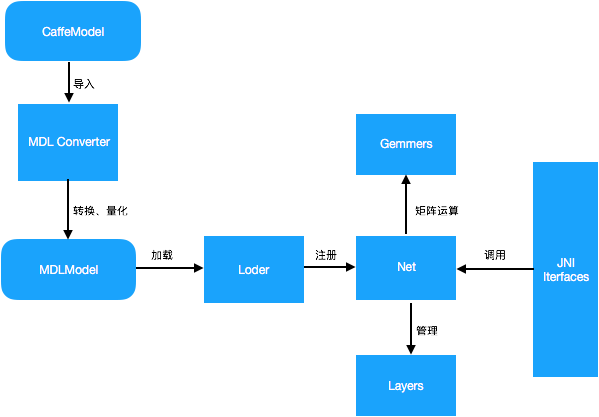
\includegraphics{./img/ch17/MDL1.png}
\caption{}
\end{figure}

MDL 框架主要包括:\textbf{模型转换模块(MDL
Converter)、模型加载模块(Loader)、网络管理模块(Net)、矩阵运算模块(Gemmers)及供
Android 端调用的 JNI 接口层(JNI Interfaces)。}

​ 其中,模型转换模块主要负责将Caffe 模型转为 MDL 模型,同时支持将 32bit
浮点型参数量化为 8bit
参数,从而极大地压缩模型体积;模型加载模块主要完成模型的反量化及加载校验、网络注册等过程,网络管理模块主要负责网络中各层
Layer 的初始化及管理工作;MDL 提供了供 Android 端调用的 JNI
接口层,开发者可以通过调用 JNI 接口轻松完成加载及预测过程。

6、MDL 的性能及兼容性

\begin{itemize}
% \tightlist
\item
  体积 armv7 300k+
\item
  速度 iOS GPU mobilenet 可以达到 40ms、squeezenet 可以达到 30ms
\end{itemize}

​ MDL
从立项到开源,已经迭代了一年多。移动端比较关注的多个指标都表现良好,如体积、功耗、速度。百度内部产品线在应用前也进行过多次对比,和已开源的相关项目对比,MDL
能够在保证速度和能耗的同时支持多种深度学习模型,如 mobilenet、googlenet
v1、squeezenet 等,且具有 iOS GPU 版本,squeezenet 一次运行最快可以达到
3-40ms。

\textbf{同类框架对比}

​
框架Caffe2TensorFlowncnnMDL(CPU)MDL(GPU)硬件CPUCPUCPUCPUGPU速度慢慢快快极快体积大大小小小兼容Android\&iOSAndroid\&iOSAndroid\&iOSAndroid\&iOSiOS

​ 与支持 CNN 的移动端框架对比,MDL 速度快、性能稳定、兼容性好、demo
完备。

\textbf{兼容性}

​ MDL 在 iOS 和 Android 平台均可以稳定运行,其中 iOS10 及以上平台有基于
GPU 运算的 API,性能表现非常出色,在 Android 平台则是纯 CPU
运行。高中低端机型运行状态和手机百度及其他 App 上的覆盖都有绝对优势。

​ MDL 同时也支持 Caffe 模型直接转换为 MDL 模型。

\subsubsection{17.10.5 Paddle-Mobile}\label{paddle-mobile}

1、开源时间:持续更新,已到3.0版本   

2、开源用户:百度    

3、GitHub地址:https://github.com/PaddlePaddle/paddle-mobile 

4、功能特点:

\textbf{功能特点}

\begin{itemize}
\item
  高性能支持ARM CPU
\item
  支持Mali GPU
\item
  支持Andreno GPU
\item
  支持苹果设备的GPU Metal实现
\item
  支持ZU5、ZU9等FPGA开发板
\item
  支持树莓派等arm-linux开发板
\end{itemize}

\subsubsection{17.10.6 MACE( Mobile AI Compute
Engine)}\label{mace-mobile-ai-compute-engine}

1、开源时间:2018年4月(持续更新,v0.9.0 (2018-07-20))   

2、开源用户:小米    

3、GitHub地址:https://github.com/XiaoMi/mace

4、简介:Mobile AI Compute Engine (MACE)
是一个专为移动端异构计算设备优化的深度学习前向预测框架。
MACE覆盖了常见的移动端计算设备(CPU,GPU和DSP),并且提供了完整的工具链和文档,用户借助MACE能够很方便地在移动端部署深度学习模型。MACE已经在小米内部广泛使用并且被充分验证具有业界领先的性能和稳定性。

5、MACE的基本框架:

\begin{figure}
\centering
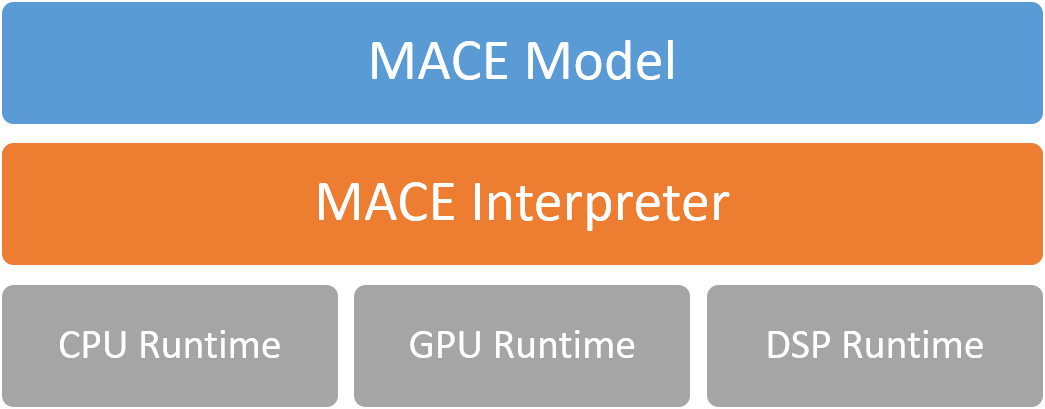
\includegraphics{./img/ch17/mace-arch.png}
\caption{}
\end{figure}

\textbf{MACE Model}

MACE定义了自有的模型格式(类似于Caffe2),通过MACE提供的工具可以将Caffe和TensorFlow的模型
转为MACE模型。

\textbf{MACE Interpreter}

MACE Interpreter主要负责解析运行神经网络图(DAG)并管理网络中的Tensors。

\textbf{Runtime}

CPU/GPU/DSP Runtime对应于各个计算设备的算子实现。

6、MACE使用的基本流程

\begin{figure}
\centering
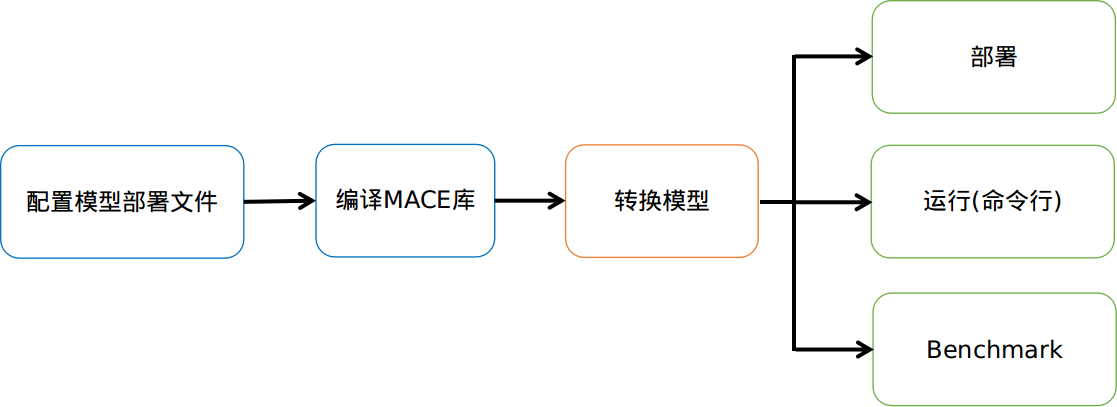
\includegraphics{./img/ch17/mace-work-flow-zh.png}
\caption{}
\end{figure}

\textbf{1. 配置模型部署文件(.yml)}

模型部署文件详细描述了需要部署的模型以及生成库的信息,MACE根据该文件最终生成对应的库文件。

\textbf{2.编译MACE库}

编译MACE的静态库或者动态库。

\textbf{3.转换模型}

将TensorFlow 或者 Caffe的模型转为MACE的模型。

\textbf{4.1. 部署}

根据不同使用目的集成Build阶段生成的库文件,然后调用MACE相应的接口执行模型。

\textbf{4.2. 命令行运行}

MACE提供了命令行工具,可以在命令行运行模型,可以用来测试模型运行时间,内存占用和正确性。

\textbf{4.3. Benchmark}

MACE提供了命令行benchmark工具,可以细粒度的查看模型中所涉及的所有算子的运行时间。

7、MACE在哪些角度进行了优化?

\textbf{MACE}
专为移动端异构计算平台优化的神经网络计算框架。主要从以下的角度做了专门的优化:

\begin{itemize}
\item
  性能
\item
  代码经过NEON指令,OpenCL以及Hexagon HVX专门优化,并且采用
  \href{https://arxiv.org/abs/1509.09308}{Winograd算法}来进行卷积操作的加速。
  此外,还对启动速度进行了专门的优化。
\item
  功耗
\item
  支持芯片的功耗管理,例如ARM的big.LITTLE调度,以及高通Adreno
  GPU功耗选项。
\item
  系统响应
\item
  支持自动拆解长时间的OpenCL计算任务,来保证UI渲染任务能够做到较好的抢占调度,
  从而保证系统UI的相应和用户体验。
\item
  内存占用
\item
  通过运用内存依赖分析技术,以及内存复用,减少内存的占用。另外,保持尽量少的外部
  依赖,保证代码尺寸精简。
\item
  模型加密与保护
\item
  模型保护是重要设计目标之一。支持将模型转换成C++代码,以及关键常量字符混淆,增加逆向的难度。
\item
  硬件支持范围
\item
  支持高通,联发科,以及松果等系列芯片的CPU,GPU与DSP(目前仅支持Hexagon)计算加速。
\item
  同时支持在具有POSIX接口的系统的CPU上运行。
\end{itemize}

8、性能对比:

MACE 支持 TensorFlow 和 Caffe
模型,提供转换工具,可以将训练好的模型转换成专有的模型数据文件,同时还可以选择将模型转换成C++代码,支持生成动态库或者静态库,提高模型保密性。

\begin{figure}
\centering
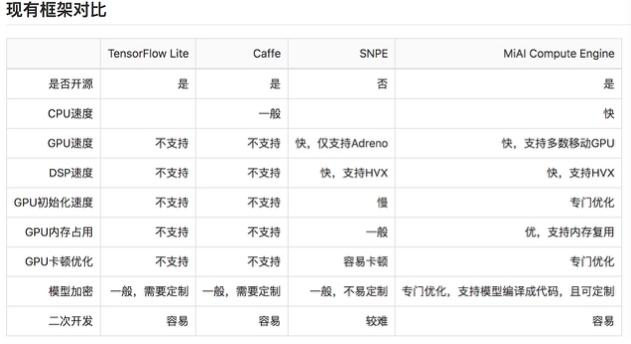
\includegraphics{./img/ch17/maca_com.jpg}
\caption{}
\end{figure}

\subsubsection{17.10.7 FeatherCNN}\label{feathercnn}

1、开源时间:持续更新,已到3.0版本   

2、开源用户:腾讯AI    

3、GitHub地址:https://github.com/Tencent/FeatherCNN

4、功能特点:

\textbf{FeatherCNN 是由腾讯 AI 平台部研发的基于 ARM 架构的高效 CNN
推理库,该项目支持 Caffe 模型,且具有高性能、易部署、轻量级三大特性。}

\textbf{该项目具体特性如下:}

\begin{itemize}
\item
  高性能:无论是在移动设备(iOS / Android),嵌入式设备(Linux)还是基于
  ARM 的服务器(Linux)上,FeatherCNN 均能发挥最先进的推理计算性能;
\item
  易部署:FeatherCNN
  的所有内容都包含在一个代码库中,以消除第三方依赖关系。因此,它便于在移动平台上部署。FeatherCNN
  自身的模型格式与 Caffe 模型完全兼容。
\item
  轻量级:编译后的 FeatherCNN 库的体积仅为数百 KB。
\end{itemize}

\subsubsection{17.10.8 TensorFlow Lite}\label{tensorflow-lite}

1、开源时间:2017年11月   

2、开源用户:谷歌   

3、GitHub地址:https://github.com/tensorflow/tensorflow/tree/master/tensorflow/contrib/lite

4、简介:

Google 表示 Lite 版本 TensorFlow 是 TensorFlow Mobile
的一个延伸版本。此前,通过TensorFlow Mobile
API,TensorFlow已经支持手机上的模型嵌入式部署。TensorFlow
Lite应该被视为TensorFlow Mobile的升级版。

TensorFlow Lite可以与Android
8.1中发布的神经网络API完美配合,即便在没有硬件加速时也能调用CPU处理,确保模型在不同设备上的运行。
而Android端版本演进的控制权是掌握在谷歌手中的,从长期看,TensorFlow
Lite会得到Android系统层面上的支持。

5、架构:

\begin{figure}
\centering
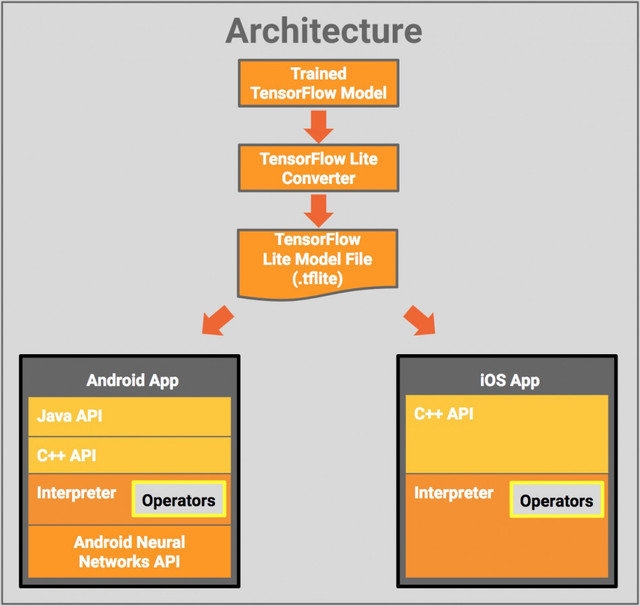
\includegraphics{./img/ch17/tflite_artc.JPEG}
\caption{}
\end{figure}

其组件包括:

\begin{itemize}
% \tightlist
\item
  TensorFlow 模型(TensorFlow Model):保存在磁盘中的训练模型。
\item
  TensorFlow Lite 转化器(TensorFlow Lite Converter):将模型转换成
  TensorFlow Lite 文件格式的项目。
\item
  TensorFlow Lite 模型文件(TensorFlow Lite Model File):基于
  FlatBuffers,适配最大速度和最小规模的模型。
\end{itemize}

6、移动端开发步骤:

Android Studio 3.0, SDK Version API26, NDK Version 14

步骤: 1. 将此项目导入到Android Studio:
https://github.com/tensorflow/tensorflow/tree/master/tensorflow/contrib/lite/java/demo

\begin{enumerate}
\def\labelenumi{\arabic{enumi}.}
\setcounter{enumi}{1}
\item
  下载移动端的模型(model)和标签数据(lables):
  https://storage.googleapis.com/download.tensorflow.org/models/tflite/mobilenet\_v1\_224\_android\_quant\_2017\_11\_08.zip
\item
  下载完成解压mobilenet\_v1\_224\_android\_quant\_2017\_11\_08.zip文件得到一个xxx.tflite和labes.txt文件,分别是模型和标签文件,并且把这两个文件复制到assets文件夹下。
\item
  构建app,run\ldots{}\ldots{}
\end{enumerate}

17.7.9 TensorFlow Lite和TensorFlow Mobile的区别?

\begin{itemize}
% \tightlist
\item
  TensorFlow Lite是TensorFlow Mobile的进化版。
\item
  在大多数情况下,TensorFlow
  Lite拥有跟小的二进制大小,更少的依赖以及更好的性能。
\item
  相比TensorFlow Mobile是对完整TensorFlow的裁减,TensorFlow
  Lite基本就是重新实现了。从内部实现来说,在TensorFlow内核最基本的OP,Context等数据结构,都是新的。从外在表现来说,模型文件从PB格式改成了FlatBuffers格式,TensorFlow的size有大幅度优化,降至300K,然后提供一个converter将普通TensorFlow模型转化成TensorFlow
  Lite需要的格式。因此,无论从哪方面看,TensorFlow
  Lite都是一个新的实现方案。
\end{itemize}

\subsubsection{17.10.9 PocketFlow}\label{pocketflow}

1、开源时间:2018年9月   

2、开源用户:腾讯   

3、GitHub地址:https://github.com/Tencent/PocketFlow

4、简介:

全球首个自动模型压缩框架

一款面向移动端AI开发者的自动模型压缩框架,集成了当前主流的模型压缩与训练算法,结合自研超参数优化组件实现了全程自动化托管式的模型压缩与加速。开发者无需了解具体算法细节,即可快速地将AI技术部署到移动端产品上,实现了自动托管式模型压缩与加速,实现用户数据的本地高效处理。

5、框架介绍

PocketFlow
框架主要由两部分组件构成,分别是模型压缩/加速算法组件和超参数优化组件,具体结构如下图所示。

\begin{figure}
\centering
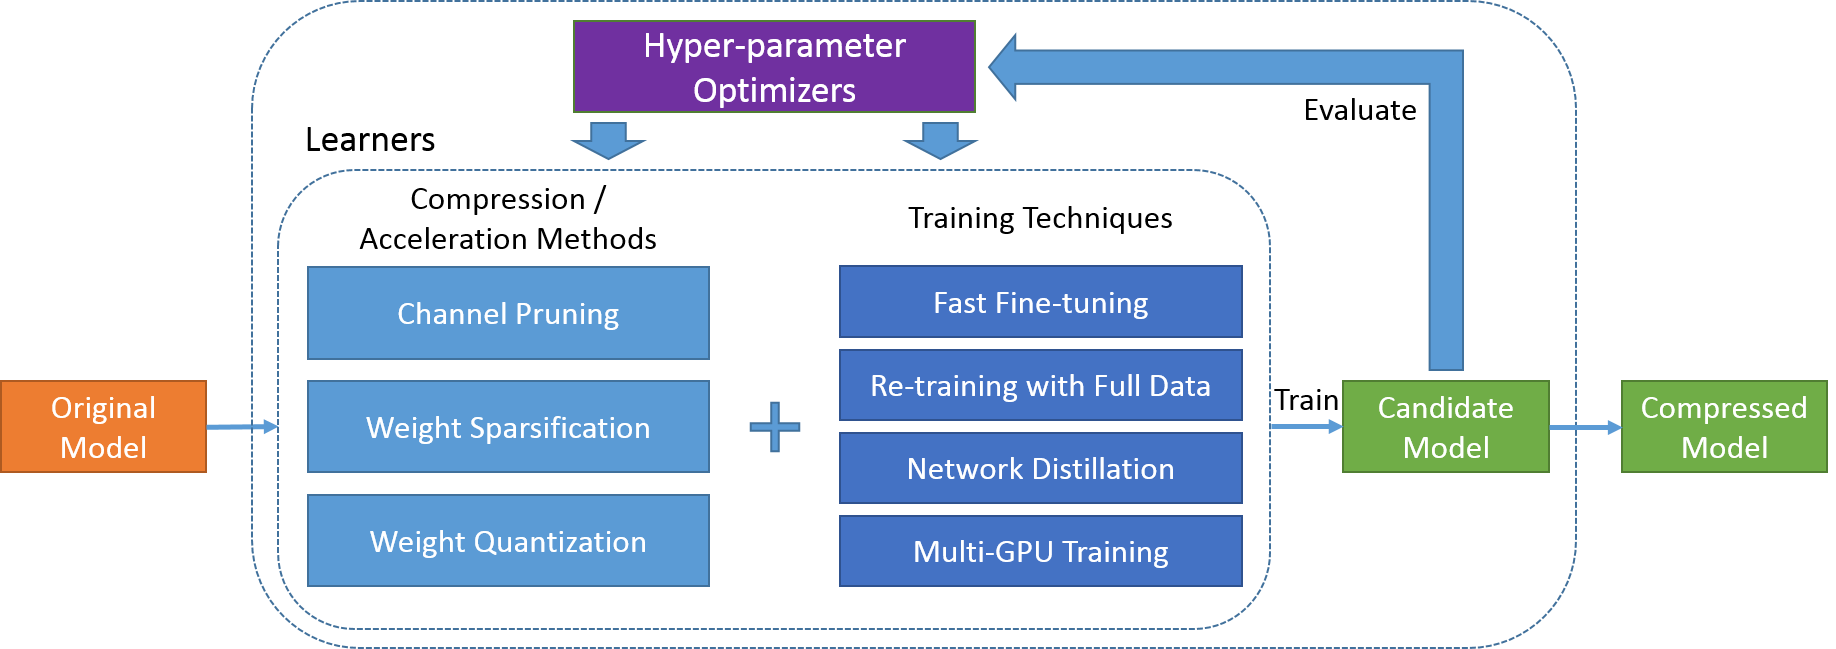
\includegraphics{./img/ch17/framework_design.png}
\caption{}
\end{figure}

​ 开发者将未压缩的原始模型作为 PocketFlow
框架的输入,同时指定期望的性能指标,例如模型的压缩和/或加速倍数;在每一轮迭代过程中,超参数优化组件选取一组超参数取值组合,之后模型压缩/加速算法组件基于该超参数取值组合,对原始模型进行压缩,得到一个压缩后的候选模型;基于对候选模型进行性能评估的结果,超参数优化组件调整自身的模型参数,并选取一组新的超参数取值组合,以开始下一轮迭代过程;当迭代终止时,PocketFlow
选取最优的超参数取值组合以及对应的候选模型,作为最终输出,返回给开发者用作移动端的模型部署。

6、PocketFlow如何实现模型压缩与加速?

​ 具体地,PocketFlow
通过下列各个算法组件的有效结合,实现了精度损失更小、自动化程度更高的深度学习模型的压缩与加速:

\begin{itemize}
\item
  \begin{enumerate}
  \def\labelenumi{\alph{enumi})}
  % \tightlist
  \item
    通道剪枝(channel
    pruning)组件:在CNN网络中,通过对特征图中的通道维度进行剪枝,可以同时降低模型大小和计算复杂度,并且压缩后的模型可以直接基于现有的深度学习框架进行部署。在CIFAR-10图像分类任务中,通过对
    ResNet-56
    模型进行通道剪枝,可以实现2.5倍加速下分类精度损失0.4\%,3.3倍加速下精度损失0.7\%。
  \end{enumerate}
\item
  \begin{enumerate}
  \def\labelenumi{\alph{enumi})}
  \setcounter{enumi}{1}
  % \tightlist
  \item
    权重稀疏化(weight
    sparsification)组件:通过对网络权重引入稀疏性约束,可以大幅度降低网络权重中的非零元素个数;压缩后模型的网络权重可以以稀疏矩阵的形式进行存储和传输,从而实现模型压缩。对于
    MobileNet 图像分类模型,在删去50\%网络权重后,在 ImageNet 数据集上的
    Top-1 分类精度损失仅为0.6\%。
  \end{enumerate}
\item
  \begin{enumerate}
  \def\labelenumi{\alph{enumi})}
  \setcounter{enumi}{2}
  % \tightlist
  \item
    权重量化(weight
    quantization)组件:通过对网络权重引入量化约束,可以降低用于表示每个网络权重所需的比特数;团队同时提供了对于均匀和非均匀两大类量化算法的支持,可以充分利用
    ARM 和 FPGA
    等设备的硬件优化,以提升移动端的计算效率,并为未来的神经网络芯片设计提供软件支持。以用于
    ImageNet 图像分类任务的 ResNet-18
    模型为例,在8比特定点量化下可以实现精度无损的4倍压缩。
  \end{enumerate}
\item
  d)网络蒸馏(network
  distillation)组件:对于上述各种模型压缩组件,通过将未压缩的原始模型的输出作为额外的监督信息,指导压缩后模型的训练,在压缩/加速倍数不变的前提下均可以获得0.5\%-2.0\%不等的精度提升。
\item
  \begin{enumerate}
  \def\labelenumi{\alph{enumi})}
  \setcounter{enumi}{4}
  % \tightlist
  \item
    多GPU训练(multi-GPU
    training)组件:深度学习模型训练过程对计算资源要求较高,单个GPU难以在短时间内完成模型训练,因此团队提供了对于多机多卡分布式训练的全面支持,以加快使用者的开发流程。无论是基于
    ImageNet 数据的Resnet-50图像分类模型还是基于 WMT14 数据的
    Transformer 机器翻译模型,均可以在一个小时内训练完毕。{[}1{]}
  \end{enumerate}
\item
  \begin{enumerate}
  \def\labelenumi{\alph{enumi})}
  \setcounter{enumi}{5}
  % \tightlist
  \item
    超参数优化(hyper-parameter
    optimization)组件:多数开发者对模型压缩算法往往不甚了解,但超参数取值对最终结果往往有着巨大的影响,因此团队引入了超参数优化组件,采用了包括强化学习等算法以及
    AI Lab 自研的 AutoML
    自动超参数优化框架来根据具体性能需求,确定最优超参数取值组合。例如,对于通道剪枝算法,超参数优化组件可以自动地根据原始模型中各层的冗余程度,对各层采用不同的剪枝比例,在保证满足模型整体压缩倍数的前提下,实现压缩后模型识别精度的最大化。
  \end{enumerate}
\end{itemize}

\begin{figure}
\centering
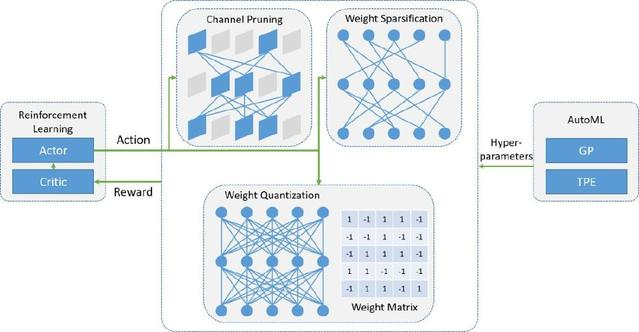
\includegraphics{./img/ch17/packflow1.jpg}
\caption{}
\end{figure}

7、PocketFlow 性能

​
通过引入超参数优化组件,不仅避免了高门槛、繁琐的人工调参工作,同时也使得
PocketFlow
在各个压缩算法上全面超过了人工调参的效果。以图像分类任务为例,在
CIFAR-10 和 ImageNet 等数据集上,PocketFlow 对 ResNet 和 MobileNet
等多种 CNN 网络结构进行有效的模型压缩与加速。

​ 在 CIFAR-10 数据集上,PocketFlow 以 ResNet-56
作为基准模型进行通道剪枝,并加入了超参数优化和网络蒸馏等训练策略,实现了
2.5 倍加速下分类精度损失 0.4\%,3.3 倍加速下精度损失
0.7\%,且显著优于未压缩的 ResNet-44 模型; 在 ImageNet
数据集上,PocketFlow 可以对原本已经十分精简的 MobileNet
模型继续进行权重稀疏化,以更小的模型尺寸取得相似的分类精度;与
Inception-V1、ResNet-18 等模型相比,模型大小仅为后者的约
20\textasciitilde{}40\%,但分类精度基本一致(甚至更高)。

\begin{figure}
\centering
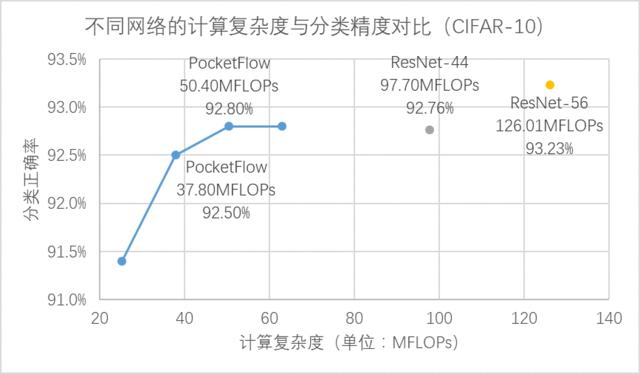
\includegraphics{./img/ch17/packflow2.jpg}
\caption{}
\end{figure}

\begin{figure}
\centering
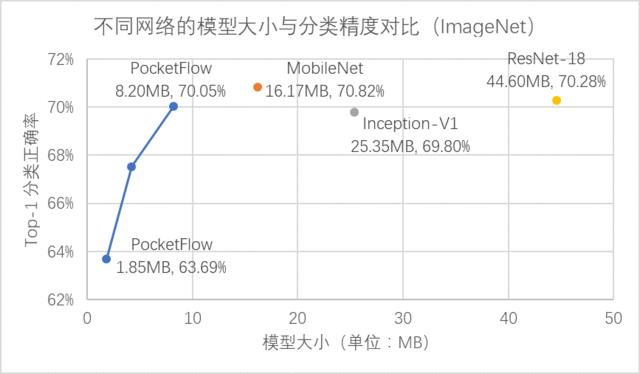
\includegraphics{./img/ch17/packflow3.jpg}
\caption{}
\end{figure}

相比于费时费力的人工调参,PocketFlow 框架中的 AutoML
自动超参数优化组件仅需 10 余次迭代就能达到与人工调参类似的性能,在经过
100 次迭代后搜索得到的超参数组合可以降低约 0.6\%
的精度损失;通过使用超参数优化组件自动地确定网络中各层权重的量化比特数,PocketFlow
在对用于 ImageNet 图像分类任务的 ResNet-18
模型进行压缩时,取得了一致性的性能提升;当平均量化比特数为 4
比特时,超参数优化组件的引入可以将分类精度从 63.6\% 提升至
68.1\%(原始模型的分类精度为 70.3\%)。

\begin{figure}
\centering
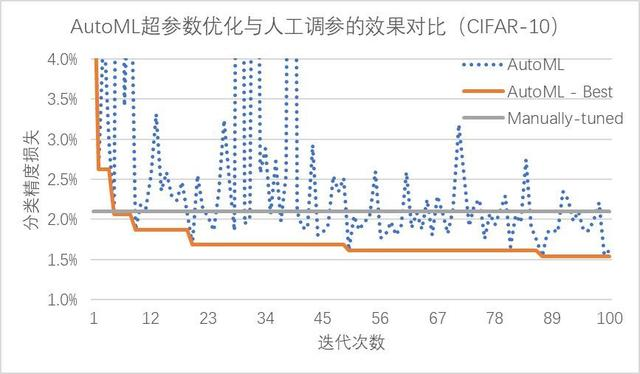
\includegraphics{./img/ch17/packflow4.jpg}
\caption{}
\end{figure}

\begin{figure}
\centering
\includegraphics{./img/ch17/packflow5.jpg}
\caption{}
\end{figure}

\textbf{参考文献}

{[}1{]} Zhuangwei Zhuang, Mingkui Tan, Bohan Zhuang, Jing Liu, Jiezhang
Cao, Qingyao Wu, Junzhou Huang, Jinhui Zhu,「Discrimination-aware
Channel Pruning for Deep Neural Networks``, In Proc. of the 32nd Annual
Conference on Neural Information Processing Systems, NIPS '18, Montreal,
Canada, December 2018.

{[}2{]} Jiaxiang Wu, Weidong Huang, Junzhou Huang, Tong Zhang,「Error
Compensated Quantized SGD and its Applications to Large-scale
Distributed Optimization」, In Proc. of the 35th International
Conference on Machine Learning, ICML'18, Stockholm, Sweden, July 2018.

\subsubsection{17.10.10
其他几款支持移动端深度学习的开源框架}\label{ux5176ux4ed6ux51e0ux6b3eux652fux6301ux79fbux52a8ux7aefux6df1ux5ea6ux5b66ux4e60ux7684ux5f00ux6e90ux6846ux67b6}

https://blog.csdn.net/zchang81/article/details/74280019

\subsubsection{17.10.11 MDL、NCNN和
TFLite比较}\label{mdlncnnux548c-tfliteux6bd4ux8f83}

百度-MDL框架、腾讯-NCNN框架和谷歌TFLite框架比较。

\begin{longtable}[]{ cccc }
\toprule
& MDL & NCNN & TFLite\tabularnewline
\midrule
\endhead
代码质量 & 中 & 高 & 很高\tabularnewline
跨平台 & √ & √ & √\tabularnewline
支持caffe模型 & √ & √ & ×\tabularnewline
支持TensorFlow模型 & × & × & √\tabularnewline
CPU NEON指令优化 & √ & √ & √\tabularnewline
GPU加速 & √ & × & ×\tabularnewline
\bottomrule
\end{longtable}

相同点:

\begin{itemize}
% \tightlist
\item
  只含推理(inference)功能,使用的模型文件需要通过离线的方式训练得到。
\item
  最终生成的库尺寸较小,均小于500kB。
\item
  为了提升执行速度,都使用了ARM NEON指令进行加速。
\item
  跨平台,iOS和Android系统都支持。
\end{itemize}

不同点:

\begin{itemize}
% \tightlist
\item
  MDL和NCNN均是只支持Caffe框架生成的模型文件,而TfLite则毫无意外的只支持自家大哥TensorFlow框架生成的模型文件。
\item
  MDL支持利用iOS系统的Matal框架进行GPU加速,能够显著提升在iPhone上的运行速度,达到准实时的效果。而NCNN和TFLite还没有这个功能。
\end{itemize}

\subsection{17.11
移动端开源框架部署}\label{ux79fbux52a8ux7aefux5f00ux6e90ux6846ux67b6ux90e8ux7f72}

\subsubsection{17.8.1 以NCNN为例}\label{ux4ee5ncnnux4e3aux4f8b}

部署步骤

\subsubsection{17.8.2 以QNNPACK为例}\label{ux4ee5qnnpackux4e3aux4f8b}

部署步骤

\subsubsection{17.8.4
在Android手机上使用MACE实现图像分类}\label{ux5728androidux624bux673aux4e0aux4f7fux7528maceux5b9eux73b0ux56feux50cfux5206ux7c7b}

\subsubsection{17.8.3
在Android手机上使用PaddleMobile实现图像分类}\label{ux5728androidux624bux673aux4e0aux4f7fux7528paddlemobileux5b9eux73b0ux56feux50cfux5206ux7c7b}

\textbf{编译paddle-mobile库}

1)编译Android能够使用的CPP库:编译Android的paddle-mobile库,可选择使用Docker编译和Ubuntu交叉编译,这里介绍使用Ubuntu交叉编译paddle-mobile库。

\emph{注}:在Android项目,Java代码调用CPP代码,CPP的函数需要遵循一定的命名规范,比如Java\_包名\_类名\_对应的Java的方法名。

​
目前官方提供了5个可以给Java调用的函数,该代码在:paddle-mobile/src/jni/paddle\_mobile\_jni.cpp,如果想要让这些函数能够在自己的包名下的类调用,就要修改CPP的函数名称修改如下:

\begin{Shaded}
\begin{Highlighting}[]
\NormalTok{JNIEXPORT jboolean JNICALL }\FunctionTok{Java_com_baidu_paddle_PML_load}\NormalTok{(JNIEnv *env, }
\NormalTok{    jclass thiz,}
\NormalTok{    jstring modelPath) \{ }
        \FunctionTok{ANDROIDLOGI}\NormalTok{(}\StringTok{"load invoked"}\NormalTok{); }
\NormalTok{        bool optimize = }\KeywordTok{true}\NormalTok{; }
        \KeywordTok{return} \FunctionTok{getPaddleMobileInstance}\NormalTok{()->}\FunctionTok{Load}\NormalTok{(}\FunctionTok{jstring2cppstring}\NormalTok{(env, modelPath), optimize); \}}
\end{Highlighting}
\end{Shaded}

​
笔者项目的包名为\texttt{com.example.paddlemobile1},在这个包下有一个\texttt{ImageRecognition.java}的程序来对应这个CPP程序,那么修改\texttt{load}函数如下:

\begin{Shaded}
\begin{Highlighting}[]
\NormalTok{JNIEXPORT jboolean JNICALL }\FunctionTok{Java_com_example_paddlemobile1_ImageRecognition_load}\NormalTok{(JNIEnv *env,}
\NormalTok{                                                          jclass thiz,}
\NormalTok{                                                          jstring modelPath) \{}
  \FunctionTok{ANDROIDLOGI}\NormalTok{(}\StringTok{"load invoked"}\NormalTok{);}
\NormalTok{  bool optimize = }\KeywordTok{true}\NormalTok{;}
  \KeywordTok{return} \FunctionTok{getPaddleMobileInstance}\NormalTok{()->}\FunctionTok{Load}\NormalTok{(}\FunctionTok{jstring2cppstring}\NormalTok{(env, modelPath),}
\NormalTok{                                         optimize);}
\NormalTok{\}}
\end{Highlighting}
\end{Shaded}

\textbf{使用Ubuntu交叉编译paddle-mobile库}

1、下载和解压NDK。

\begin{verbatim}
wget https://dl.google.com/android/repository/android-ndk-r17b-linux-x86_64.zip
unzip android-ndk-r17b-linux-x86_64.zip
\end{verbatim}

2、设置NDK环境变量,目录是NDK的解压目录。

\begin{verbatim}
export NDK_ROOT="/home/test/paddlepaddle/android-ndk-r17b"
\end{verbatim}

设置好之后,可以使用以下的命令查看配置情况。

\begin{verbatim}
root@test:/home/test/paddlepaddle# echo $NDK_ROOT
/home/test/paddlepaddle/android-ndk-r17b
\end{verbatim}

3、安装cmake,需要安装较高版本的,笔者的cmake版本是3.11.2。

下载cmake源码

\begin{verbatim}
wget https://cmake.org/files/v3.11/cmake-3.11.2.tar.gz
\end{verbatim}

解压cmake源码

\begin{verbatim}
tar -zxvf cmake-3.11.2.tar.gz
\end{verbatim}

进入到cmake源码根目录,并执行bootstrap。

\begin{verbatim}
cd cmake-3.11.2
./bootstrap
\end{verbatim}

最后执行以下两条命令开始安装cmake。

\begin{verbatim}
make
make install
\end{verbatim}

安装完成之后,可以使用cmake --version是否安装成功.

\begin{verbatim}
root@test:/home/test/paddlepaddle# cmake --version
cmake version 3.11.2

CMake suite maintained and supported by Kitware (kitware.com/cmake).
\end{verbatim}

4、克隆paddle-mobile源码。

\begin{verbatim}
git clone https://github.com/PaddlePaddle/paddle-mobile.git
\end{verbatim}

5、进入到paddle-mobile的tools目录下,执行编译。

\begin{verbatim}
cd paddle-mobile/tools/
sh build.sh android
\end{verbatim}

(可选)如果想编译针对某一个网络编译更小的库时,可以在命令后面加上相应的参数,如下:

\begin{verbatim}
sh build.sh android googlenet
\end{verbatim}

6、最后会在paddle-mobile/build/release/arm-v7a/build目录下生产paddle-mobile库。

\begin{Shaded}
\begin{Highlighting}[]
\NormalTok{root}\AttributeTok{@test}\NormalTok{:/home/test/paddlepaddle/paddle-mobile/build/release/arm-v7a/build# ls}
\NormalTok{libpaddle-mobile.}\FunctionTok{so}
\end{Highlighting}
\end{Shaded}

libpaddle-mobile.so就是我们在开发Android项目的时候使用到的paddle-mobile库。

\textbf{创建Android项目}

1、首先使用Android
Studio创建一个普通的Android项目,包名为\texttt{com.example.paddlemobile1}

2、在main目录下创建l两个assets/paddle\_models文件夹,这个文件夹存放PaddleFluid训练好的预测模型。PaddleMobile支持量化模型,使用模型量化可以把模型缩小至原来的四分之一,如果使用量化模型,那加载模型的接口也有修改一下,使用以下的接口加载模型:

\begin{Shaded}
\begin{Highlighting}[]
\KeywordTok{public} \DataTypeTok{static} \KeywordTok{native} \DataTypeTok{boolean} \FunctionTok{loadQualified}\NormalTok{(}\BuiltInTok{String}\NormalTok{ modelDir);}
\end{Highlighting}
\end{Shaded}

3、在\texttt{main}目录下创建一个\texttt{jniLibs}文件夹,这个文件夹是存放CPP编译库的,在本项目中就存放上一部分编译的\texttt{libpaddle-mobile.so}

4、在Android项目的配置文件夹中加上权限声明,因为我们要使用到读取相册和使用相机,所以加上以下的权限声明:

\begin{Shaded}
\begin{Highlighting}[]
\NormalTok{<uses-permission android:name=}\StringTok{"android.permission.CAMERA"}\NormalTok{ />}
\NormalTok{<uses-permission android:name=}\StringTok{"android.permission.WRITE_EXTERNAL_STORAGE"}\NormalTok{ />}
\NormalTok{<uses-permission android:name=}\StringTok{"android.permission.READ_EXTERNAL_STORAGE"}\NormalTok{ />}
\end{Highlighting}
\end{Shaded}

5、修改\texttt{activity\_main.xml}界面,修改成如下:

\begin{Shaded}
\begin{Highlighting}[]
\NormalTok{<?xml version=}\StringTok{"1.0"}\NormalTok{ encoding=}\StringTok{"utf-8"}\NormalTok{?>}
\NormalTok{<RelativeLayout xmlns:android=}\StringTok{"http://schemas.android.com/apk/res/android"}
\NormalTok{    xmlns:app=}\StringTok{"http://schemas.android.com/apk/res-auto"}
\NormalTok{    xmlns:tools=}\StringTok{"http://schemas.android.com/tools"}
\NormalTok{    android:layout_width=}\StringTok{"match_parent"}
\NormalTok{    android:layout_height=}\StringTok{"match_parent"}
\NormalTok{    tools:context=}\StringTok{".MainActivity"}\NormalTok{>}
\NormalTok{<LinearLayout}
\NormalTok{    android:id=}\StringTok{"@+id/btn_ll"}
\NormalTok{    android:layout_alignParentBottom=}\StringTok{"true"}
\NormalTok{    android:layout_width=}\StringTok{"match_parent"}
\NormalTok{    android:layout_height=}\StringTok{"wrap_content"}
\NormalTok{    android:orientation=}\StringTok{"horizontal"}\NormalTok{>}

\NormalTok{    <}\BuiltInTok{Button}
\NormalTok{        android:id=}\StringTok{"@+id/use_photo"}
\NormalTok{        android:layout_weight=}\StringTok{"1"}
\NormalTok{        android:layout_width=}\StringTok{"0dp"}
\NormalTok{        android:layout_height=}\StringTok{"wrap_content"}
\NormalTok{        android:text=}\StringTok{"相册"}\NormalTok{ />}

\NormalTok{    <}\BuiltInTok{Button}
\NormalTok{        android:id=}\StringTok{"@+id/start_camera"}
\NormalTok{        android:layout_weight=}\StringTok{"1"}
\NormalTok{        android:layout_width=}\StringTok{"0dp"}
\NormalTok{        android:layout_height=}\StringTok{"wrap_content"}
\NormalTok{        android:text=}\StringTok{"拍照"}\NormalTok{ />}
\NormalTok{</LinearLayout>}

\NormalTok{<TextView}
\NormalTok{    android:layout_above=}\StringTok{"@id/btn_ll"}
\NormalTok{    android:id=}\StringTok{"@+id/result_text"}
\NormalTok{    android:textSize=}\StringTok{"16sp"}
\NormalTok{    android:layout_width=}\StringTok{"match_parent"}
\NormalTok{    android:hint=}\StringTok{"预测结果会在这里显示"}
\NormalTok{    android:layout_height=}\StringTok{"100dp"}\NormalTok{ />}

\NormalTok{<}\BuiltInTok{ImageView}
\NormalTok{    android:layout_alignParentTop=}\StringTok{"true"}
\NormalTok{    android:layout_above=}\StringTok{"@id/result_text"}
\NormalTok{    android:id=}\StringTok{"@+id/show_image"}
\NormalTok{    android:layout_width=}\StringTok{"match_parent"}
\NormalTok{    android:layout_height=}\StringTok{"match_parent"}\NormalTok{ />}
\NormalTok{</RelativeLayout>}
\end{Highlighting}
\end{Shaded}

6、创建一个\texttt{ImageRecognition.java}的Java程序,这个程序的作用就是调用\texttt{paddle-mobile/src/jni/paddle\_mobile\_jni.cpp}的函数,对应的是里面的函数。目前支持一下几个接口。

\begin{Shaded}
\begin{Highlighting}[]
\KeywordTok{package}\ImportTok{ com.example.paddlemobile1;}

\KeywordTok{public} \KeywordTok{class}\NormalTok{ ImageRecognition \{}
    \CommentTok{// set thread num}
    \KeywordTok{public} \DataTypeTok{static} \KeywordTok{native} \DataTypeTok{void} \FunctionTok{setThread}\NormalTok{(}\DataTypeTok{int}\NormalTok{ threadCount);}

\CommentTok{//Load seperated parameters}
\KeywordTok{public} \DataTypeTok{static} \KeywordTok{native} \DataTypeTok{boolean} \FunctionTok{load}\NormalTok{(}\BuiltInTok{String}\NormalTok{ modelDir);}

\CommentTok{// load qualified model}
\KeywordTok{public} \DataTypeTok{static} \KeywordTok{native} \DataTypeTok{boolean} \FunctionTok{loadQualified}\NormalTok{(}\BuiltInTok{String}\NormalTok{ modelDir);}

\CommentTok{// Load combined parameters}
\KeywordTok{public} \DataTypeTok{static} \KeywordTok{native} \DataTypeTok{boolean} \FunctionTok{loadCombined}\NormalTok{(}\BuiltInTok{String}\NormalTok{ modelPath, }\BuiltInTok{String}\NormalTok{ paramPath);}

\CommentTok{// load qualified model}
\KeywordTok{public} \DataTypeTok{static} \KeywordTok{native} \DataTypeTok{boolean} \FunctionTok{loadCombinedQualified}\NormalTok{(}\BuiltInTok{String}\NormalTok{ modelPath, }\BuiltInTok{String}\NormalTok{ paramPath);}

\CommentTok{// object detection}
\KeywordTok{public} \DataTypeTok{static} \KeywordTok{native} \DataTypeTok{float}\NormalTok{[] }\FunctionTok{predictImage}\NormalTok{(}\DataTypeTok{float}\NormalTok{[] buf, }\DataTypeTok{int}\NormalTok{[]ddims);}

\CommentTok{// predict yuv image}
\KeywordTok{public} \DataTypeTok{static} \KeywordTok{native} \DataTypeTok{float}\NormalTok{[] }\FunctionTok{predictYuv}\NormalTok{(}\DataTypeTok{byte}\NormalTok{[] buf, }\DataTypeTok{int}\NormalTok{ imgWidth, }\DataTypeTok{int}\NormalTok{ imgHeight, }\DataTypeTok{int}\NormalTok{[] ddims, }\DataTypeTok{float}\NormalTok{[]meanValues);}

\CommentTok{// clear model}
\KeywordTok{public} \DataTypeTok{static} \KeywordTok{native} \DataTypeTok{void} \FunctionTok{clear}\NormalTok{();}
\NormalTok{\}}
\end{Highlighting}
\end{Shaded}

7、然后编写一个\texttt{PhotoUtil.java}的工具类。

\begin{Shaded}
\begin{Highlighting}[]
\KeywordTok{package}\ImportTok{ com.example.paddlemobile1;}

\KeywordTok{import}\ImportTok{ android.app.Activity;}
\KeywordTok{import}\ImportTok{ android.content.Context;}
\KeywordTok{import}\ImportTok{ android.content.Intent;}
\KeywordTok{import}\ImportTok{ android.database.Cursor;}
\KeywordTok{import}\ImportTok{ android.graphics.Bitmap;}
\KeywordTok{import}\ImportTok{ android.graphics.BitmapFactory;}
\KeywordTok{import}\ImportTok{ android.net.Uri;}
\KeywordTok{import}\ImportTok{ android.os.Build;}
\KeywordTok{import}\ImportTok{ android.provider.MediaStore;}
\KeywordTok{import}\ImportTok{ android.support.v4.content.FileProvider;}
\KeywordTok{import}\ImportTok{ android.util.Log;}

\KeywordTok{import}\ImportTok{ java.io.File;}
\KeywordTok{import}\ImportTok{ java.io.IOException;}
\KeywordTok{import}\ImportTok{ java.util.Arrays;}

\KeywordTok{public} \KeywordTok{class}\NormalTok{ PhotoUtil \{}
\CommentTok{// start camera}
\KeywordTok{public} \DataTypeTok{static}\NormalTok{ Uri }\FunctionTok{start_camera}\NormalTok{(Activity activity, }\DataTypeTok{int}\NormalTok{ requestCode) \{}
\NormalTok{    Uri imageUri;}
    \CommentTok{// save image in cache path}
    \BuiltInTok{File}\NormalTok{ outputImage = }\KeywordTok{new} \BuiltInTok{File}\NormalTok{(activity.}\FunctionTok{getExternalCacheDir}\NormalTok{(), }\StringTok{"out_image.jpg"}\NormalTok{);}
    \KeywordTok{try}\NormalTok{ \{}
        \KeywordTok{if}\NormalTok{ (outputImage.}\FunctionTok{exists}\NormalTok{()) \{}
\NormalTok{            outputImage.}\FunctionTok{delete}\NormalTok{();}
\NormalTok{        \}}
\NormalTok{        outputImage.}\FunctionTok{createNewFile}\NormalTok{();}
\NormalTok{    \} }\KeywordTok{catch}\NormalTok{ (}\BuiltInTok{IOException}\NormalTok{ e) \{}
\NormalTok{        e.}\FunctionTok{printStackTrace}\NormalTok{();}
\NormalTok{    \}}
    \KeywordTok{if}\NormalTok{ (Build.}\FunctionTok{VERSION}\NormalTok{.}\FunctionTok{SDK_INT}\NormalTok{ >= }\DecValTok{24}\NormalTok{) \{}
        \CommentTok{// compatible with Android 7.0 or over}
\NormalTok{        imageUri = FileProvider.}\FunctionTok{getUriForFile}\NormalTok{(activity,}
                \StringTok{"com.example.paddlemobile1"}\NormalTok{, outputImage);}
\NormalTok{    \} }\KeywordTok{else}\NormalTok{ \{}
\NormalTok{        imageUri = Uri.}\FunctionTok{fromFile}\NormalTok{(outputImage);}
\NormalTok{    \}}
    \CommentTok{// set system camera Action}
\NormalTok{    Intent intent = }\KeywordTok{new} \FunctionTok{Intent}\NormalTok{(MediaStore.}\FunctionTok{ACTION_IMAGE_CAPTURE}\NormalTok{);}
    \CommentTok{// set save photo path}
\NormalTok{    intent.}\FunctionTok{putExtra}\NormalTok{(MediaStore.}\FunctionTok{EXTRA_OUTPUT}\NormalTok{, imageUri);}
    \CommentTok{// set photo quality, min is 0, max is 1}
\NormalTok{    intent.}\FunctionTok{putExtra}\NormalTok{(MediaStore.}\FunctionTok{EXTRA_VIDEO_QUALITY}\NormalTok{, }\DecValTok{0}\NormalTok{);}
\NormalTok{    activity.}\FunctionTok{startActivityForResult}\NormalTok{(intent, requestCode);}
    \KeywordTok{return}\NormalTok{ imageUri;}
\NormalTok{\}}

\CommentTok{// get picture in photo}
\KeywordTok{public} \DataTypeTok{static} \DataTypeTok{void} \FunctionTok{use_photo}\NormalTok{(Activity activity, }\DataTypeTok{int}\NormalTok{ requestCode)\{}
\NormalTok{    Intent intent = }\KeywordTok{new} \FunctionTok{Intent}\NormalTok{(Intent.}\FunctionTok{ACTION_PICK}\NormalTok{);}
\NormalTok{    intent.}\FunctionTok{setType}\NormalTok{(}\StringTok{"image/*"}\NormalTok{);}
\NormalTok{    activity.}\FunctionTok{startActivityForResult}\NormalTok{(intent, requestCode);}
\NormalTok{\}}

\CommentTok{// get photo from Uri}
\KeywordTok{public} \DataTypeTok{static} \BuiltInTok{String} \FunctionTok{get_path_from_URI}\NormalTok{(}\BuiltInTok{Context}\NormalTok{ context, Uri uri) \{}
    \BuiltInTok{String}\NormalTok{ result;}
    \BuiltInTok{Cursor}\NormalTok{ cursor = context.}\FunctionTok{getContentResolver}\NormalTok{().}\FunctionTok{query}\NormalTok{(uri, }\KeywordTok{null}\NormalTok{, }\KeywordTok{null}\NormalTok{, }\KeywordTok{null}\NormalTok{, }\KeywordTok{null}\NormalTok{);}
    \KeywordTok{if}\NormalTok{ (cursor == }\KeywordTok{null}\NormalTok{) \{}
\NormalTok{        result = uri.}\FunctionTok{getPath}\NormalTok{();}
\NormalTok{    \} }\KeywordTok{else}\NormalTok{ \{}
\NormalTok{        cursor.}\FunctionTok{moveToFirst}\NormalTok{();}
        \DataTypeTok{int}\NormalTok{ idx = cursor.}\FunctionTok{getColumnIndex}\NormalTok{(MediaStore.}\FunctionTok{Images}\NormalTok{.}\FunctionTok{ImageColumns}\NormalTok{.}\FunctionTok{DATA}\NormalTok{);}
\NormalTok{        result = cursor.}\FunctionTok{getString}\NormalTok{(idx);}
\NormalTok{        cursor.}\FunctionTok{close}\NormalTok{();}
\NormalTok{    \}}
    \KeywordTok{return}\NormalTok{ result;}
\NormalTok{\}}

\CommentTok{// Compress the image to the size of the training image,and change RGB}
\KeywordTok{public} \DataTypeTok{static} \DataTypeTok{float}\NormalTok{[] }\FunctionTok{getScaledMatrix}\NormalTok{(Bitmap bitmap, }\DataTypeTok{int}\NormalTok{ desWidth,}
                               \DataTypeTok{int}\NormalTok{ desHeight) \{}
    \DataTypeTok{float}\NormalTok{[] dataBuf = }\KeywordTok{new} \DataTypeTok{float}\NormalTok{[}\DecValTok{3}\NormalTok{ * desWidth * desHeight];}
    \DataTypeTok{int}\NormalTok{ rIndex;}
    \DataTypeTok{int}\NormalTok{ gIndex;}
    \DataTypeTok{int}\NormalTok{ bIndex;}
    \DataTypeTok{int}\NormalTok{[] pixels = }\KeywordTok{new} \DataTypeTok{int}\NormalTok{[desWidth * desHeight];}
\NormalTok{    Bitmap bm = Bitmap.}\FunctionTok{createScaledBitmap}\NormalTok{(bitmap, desWidth, desHeight, }\KeywordTok{false}\NormalTok{);}
\NormalTok{    bm.}\FunctionTok{getPixels}\NormalTok{(pixels, }\DecValTok{0}\NormalTok{, desWidth, }\DecValTok{0}\NormalTok{, }\DecValTok{0}\NormalTok{, desWidth, desHeight);}
    \DataTypeTok{int}\NormalTok{ j = }\DecValTok{0}\NormalTok{;}
    \DataTypeTok{int}\NormalTok{ k = }\DecValTok{0}\NormalTok{;}
    \KeywordTok{for}\NormalTok{ (}\DataTypeTok{int}\NormalTok{ i = }\DecValTok{0}\NormalTok{; i < pixels.}\FunctionTok{length}\NormalTok{; i++) \{}
        \DataTypeTok{int}\NormalTok{ clr = pixels[i];}
\NormalTok{        j = i / desHeight;}
\NormalTok{        k = i % desWidth;}
\NormalTok{        rIndex = j * desWidth + k;}
\NormalTok{        gIndex = rIndex + desHeight * desWidth;}
\NormalTok{        bIndex = gIndex + desHeight * desWidth;}
\NormalTok{        dataBuf[rIndex] = (}\DataTypeTok{float}\NormalTok{) ((clr & }\BaseNTok{0x00ff0000}\NormalTok{) >> }\DecValTok{16}\NormalTok{) - }\DecValTok{148}\NormalTok{;}
\NormalTok{        dataBuf[gIndex] = (}\DataTypeTok{float}\NormalTok{) ((clr & }\BaseNTok{0x0000ff00}\NormalTok{) >> }\DecValTok{8}\NormalTok{) - }\DecValTok{148}\NormalTok{;}
\NormalTok{        dataBuf[bIndex] = (}\DataTypeTok{float}\NormalTok{) ((clr & }\BaseNTok{0x000000ff}\NormalTok{)) - }\DecValTok{148}\NormalTok{;}

\NormalTok{    \}}
    \KeywordTok{if}\NormalTok{ (bm.}\FunctionTok{isRecycled}\NormalTok{()) \{}
\NormalTok{        bm.}\FunctionTok{recycle}\NormalTok{();}
\NormalTok{    \}}
    \KeywordTok{return}\NormalTok{ dataBuf;}
\NormalTok{\}}

\CommentTok{// compress picture}
\KeywordTok{public} \DataTypeTok{static}\NormalTok{ Bitmap }\FunctionTok{getScaleBitmap}\NormalTok{(}\BuiltInTok{String}\NormalTok{ filePath) \{}
\NormalTok{    BitmapFactory.}\FunctionTok{Options}\NormalTok{ opt = }\KeywordTok{new}\NormalTok{ BitmapFactory.}\FunctionTok{Options}\NormalTok{();}
\NormalTok{    opt.}\FunctionTok{inJustDecodeBounds}\NormalTok{ = }\KeywordTok{true}\NormalTok{;}
\NormalTok{    BitmapFactory.}\FunctionTok{decodeFile}\NormalTok{(filePath, opt);}

    \DataTypeTok{int}\NormalTok{ bmpWidth = opt.}\FunctionTok{outWidth}\NormalTok{;}
    \DataTypeTok{int}\NormalTok{ bmpHeight = opt.}\FunctionTok{outHeight}\NormalTok{;}

    \DataTypeTok{int}\NormalTok{ maxSize = }\DecValTok{500}\NormalTok{;}

    \CommentTok{// compress picture with inSampleSize}
\NormalTok{    opt.}\FunctionTok{inSampleSize}\NormalTok{ = }\DecValTok{1}\NormalTok{;}
    \KeywordTok{while}\NormalTok{ (}\KeywordTok{true}\NormalTok{) \{}
        \KeywordTok{if}\NormalTok{ (bmpWidth / opt.}\FunctionTok{inSampleSize}\NormalTok{ < maxSize || bmpHeight / opt.}\FunctionTok{inSampleSize}\NormalTok{ < maxSize) \{}
            \KeywordTok{break}\NormalTok{;}
\NormalTok{        \}}
\NormalTok{        opt.}\FunctionTok{inSampleSize}\NormalTok{ *= }\DecValTok{2}\NormalTok{;}
\NormalTok{    \}}
\NormalTok{    opt.}\FunctionTok{inJustDecodeBounds}\NormalTok{ = }\KeywordTok{false}\NormalTok{;}
    \KeywordTok{return}\NormalTok{ BitmapFactory.}\FunctionTok{decodeFile}\NormalTok{(filePath, opt);}
\NormalTok{\}}
\NormalTok{\}}
\end{Highlighting}
\end{Shaded}

\begin{itemize}
% \tightlist
\item
  start\_camera()方法是启动相机并返回图片的URI。
\item
  use\_photo()方法是打开相册,获取到的图片URI在回到函数中获取。
\item
  get\_path\_from\_URI()方法是把图片的URI转换成绝对路径。
\item
  getScaledMatrix()方法是把图片压缩成跟训练时的大小,并转换成预测需要用的数据格式浮点数组。
\item
  getScaleBitmap()方法是对图片进行等比例压缩,减少内存的支出。
\end{itemize}

8、最后修改\texttt{MainActivity.java},修改如下:

% \begin{Shaded}
% \begin{Highlighting}[]
% \KeywordTok{package}\ImportTok{ com.example.paddlemobile1;}

% \KeywordTok{import}\ImportTok{ android.Manifest;}
% \KeywordTok{import}\ImportTok{ android.annotation.SuppressLint;}
% \KeywordTok{import}\ImportTok{ android.app.Activity;}
% \KeywordTok{import}\ImportTok{ android.content.Context;}
% \KeywordTok{import}\ImportTok{ android.content.Intent;}
% \KeywordTok{import}\ImportTok{ android.content.pm.PackageManager;}
% \KeywordTok{import}\ImportTok{ android.graphics.Bitmap;}
% \KeywordTok{import}\ImportTok{ android.net.Uri;}
% \KeywordTok{import}\ImportTok{ android.os.Bundle;}
% \KeywordTok{import}\ImportTok{ android.os.Environment;}
% \KeywordTok{import}\ImportTok{ android.support.annotation.NonNull;}
% \KeywordTok{import}\ImportTok{ android.support.annotation.Nullable;}
% \KeywordTok{import}\ImportTok{ android.support.v4.app.ActivityCompat;}
% \KeywordTok{import}\ImportTok{ android.support.v4.content.ContextCompat;}
% \KeywordTok{import}\ImportTok{ android.support.v7.app.AppCompatActivity;}
% \KeywordTok{import}\ImportTok{ android.util.Log;}
% \KeywordTok{import}\ImportTok{ android.view.View;}
% \KeywordTok{import}\ImportTok{ android.widget.Button;}
% \KeywordTok{import}\ImportTok{ android.widget.ImageView;}
% \KeywordTok{import}\ImportTok{ android.widget.TextView;}
% \KeywordTok{import}\ImportTok{ android.widget.Toast;}

% \KeywordTok{import}\ImportTok{ com.bumptech.glide.Glide;}
% \KeywordTok{import}\ImportTok{ com.bumptech.glide.load.engine.DiskCacheStrategy;}
% \KeywordTok{import}\ImportTok{ com.bumptech.glide.request.RequestOptions;}

% \KeywordTok{import}\ImportTok{ java.io.File;}
% \KeywordTok{import}\ImportTok{ java.io.FileOutputStream;}
% \KeywordTok{import}\ImportTok{ java.io.InputStream;}
% \KeywordTok{import}\ImportTok{ java.util.ArrayList;}
% \KeywordTok{import}\ImportTok{ java.util.Arrays;}
% \KeywordTok{import}\ImportTok{ java.util.List;}

% \KeywordTok{public} \KeywordTok{class}\NormalTok{ MainActivity }\KeywordTok{extends}\NormalTok{ AppCompatActivity \{}
%     \KeywordTok{private} \DataTypeTok{static} \DataTypeTok{final} \BuiltInTok{String}\NormalTok{ TAG = MainActivity.}\FunctionTok{class}\NormalTok{.}\FunctionTok{getName}\NormalTok{();}
%     \KeywordTok{private} \DataTypeTok{static} \DataTypeTok{final} \DataTypeTok{int}\NormalTok{ USE_PHOTO = }\DecValTok{1001}\NormalTok{;}
%     \KeywordTok{private} \DataTypeTok{static} \DataTypeTok{final} \DataTypeTok{int}\NormalTok{ START_CAMERA = }\DecValTok{1002}\NormalTok{;}
%     \KeywordTok{private}\NormalTok{ Uri image_uri;}
%     \KeywordTok{private} \BuiltInTok{ImageView}\NormalTok{ show_image;}
%     \KeywordTok{private}\NormalTok{ TextView result_text;}
%     \KeywordTok{private} \BuiltInTok{String}\NormalTok{ assets_path = }\StringTok{"paddle_models"}\NormalTok{;}
%     \KeywordTok{private} \DataTypeTok{boolean}\NormalTok{ load_result = }\KeywordTok{false}\NormalTok{;}
%     \KeywordTok{private} \DataTypeTok{int}\NormalTok{[] ddims = \{}\DecValTok{1}\NormalTok{, }\DecValTok{3}\NormalTok{, }\DecValTok{224}\NormalTok{, }\DecValTok{224}\NormalTok{\};}
% \KeywordTok{private} \DataTypeTok{static} \DataTypeTok{final} \BuiltInTok{String}\NormalTok{[] PADDLE_MODEL = \{}
%         \StringTok{"lenet"}\NormalTok{,}
%         \StringTok{"alexnet"}\NormalTok{,}
%         \StringTok{"vgg16"}\NormalTok{,}
%         \StringTok{"resnet"}\NormalTok{,}
%         \StringTok{"googlenet"}\NormalTok{,}
%         \StringTok{"mobilenet_v1"}\NormalTok{,}
%         \StringTok{"mobilenet_v2"}\NormalTok{,}
%         \StringTok{"inception_v1"}\NormalTok{,}
%         \StringTok{"inception_v2"}\NormalTok{,}
%         \StringTok{"squeezenet"}
% \NormalTok{\};}

% \CommentTok{// load paddle-mobile api}
% \DataTypeTok{static}\NormalTok{ \{}
%     \KeywordTok{try}\NormalTok{ \{}
%         \BuiltInTok{System}\NormalTok{.}\FunctionTok{loadLibrary}\NormalTok{(}\StringTok{"paddle-mobile"}\NormalTok{);}

% \NormalTok{    \} }\KeywordTok{catch}\NormalTok{ (}\BuiltInTok{SecurityException}\NormalTok{ e) \{}
% \NormalTok{        e.}\FunctionTok{printStackTrace}\NormalTok{();}

% \NormalTok{    \} }\KeywordTok{catch}\NormalTok{ (}\BuiltInTok{UnsatisfiedLinkError}\NormalTok{ e) \{}
% \NormalTok{        e.}\FunctionTok{printStackTrace}\NormalTok{();}

% \NormalTok{    \} }\KeywordTok{catch}\NormalTok{ (}\BuiltInTok{NullPointerException}\NormalTok{ e) \{}
% \NormalTok{        e.}\FunctionTok{printStackTrace}\NormalTok{();}

% \NormalTok{    \}}

% \NormalTok{\}}
% \end{Highlighting}
% \end{Shaded}

% \begin{Shaded}
% \begin{Highlighting}[]
% \AttributeTok{@Override}
% \KeywordTok{protected} \DataTypeTok{void} \FunctionTok{onCreate}\NormalTok{(Bundle savedInstanceState) \{}
%     \KeywordTok{super}\NormalTok{.}\FunctionTok{onCreate}\NormalTok{(savedInstanceState);}
%     \FunctionTok{setContentView}\NormalTok{(R.}\FunctionTok{layout}\NormalTok{.}\FunctionTok{activity_main}\NormalTok{);}

%     \FunctionTok{init}\NormalTok{();}
% \NormalTok{\}}

% \CommentTok{// initialize view}
% \KeywordTok{private} \DataTypeTok{void} \FunctionTok{init}\NormalTok{() \{}
%     \FunctionTok{request_permissions}\NormalTok{();}
% \NormalTok{    show_image = (}\BuiltInTok{ImageView}\NormalTok{) }\FunctionTok{findViewById}\NormalTok{(R.}\FunctionTok{id}\NormalTok{.}\FunctionTok{show_image}\NormalTok{);}
% \NormalTok{    result_text = (TextView) }\FunctionTok{findViewById}\NormalTok{(R.}\FunctionTok{id}\NormalTok{.}\FunctionTok{result_text}\NormalTok{);}
%     \BuiltInTok{Button}\NormalTok{ use_photo = (}\BuiltInTok{Button}\NormalTok{) }\FunctionTok{findViewById}\NormalTok{(R.}\FunctionTok{id}\NormalTok{.}\FunctionTok{use_photo}\NormalTok{);}
%     \BuiltInTok{Button}\NormalTok{ start_photo = (}\BuiltInTok{Button}\NormalTok{) }\FunctionTok{findViewById}\NormalTok{(R.}\FunctionTok{id}\NormalTok{.}\FunctionTok{start_camera}\NormalTok{);}

%     \CommentTok{// use photo click}
% \NormalTok{    use_photo.}\FunctionTok{setOnClickListener}\NormalTok{(}\KeywordTok{new} \BuiltInTok{View}\NormalTok{.}\FunctionTok{OnClickListener}\NormalTok{() \{}
%         \AttributeTok{@Override}
%         \KeywordTok{public} \DataTypeTok{void} \FunctionTok{onClick}\NormalTok{(}\BuiltInTok{View}\NormalTok{ view) \{}
% \NormalTok{            PhotoUtil.}\FunctionTok{use_photo}\NormalTok{(MainActivity.}\FunctionTok{this}\NormalTok{, USE_PHOTO);}
%             \CommentTok{//                load_model();}
% \NormalTok{            \}}
% \NormalTok{        \});}
% \end{Highlighting}
% \end{Shaded}

% \begin{Shaded}
% \begin{Highlighting}[]
%     \CommentTok{// start camera click}
% \NormalTok{    start_photo.}\FunctionTok{setOnClickListener}\NormalTok{(}\KeywordTok{new} \BuiltInTok{View}\NormalTok{.}\FunctionTok{OnClickListener}\NormalTok{() \{}
%         \AttributeTok{@Override}
%         \KeywordTok{public} \DataTypeTok{void} \FunctionTok{onClick}\NormalTok{(}\BuiltInTok{View}\NormalTok{ view) \{}
% \NormalTok{            image_uri = PhotoUtil.}\FunctionTok{start_camera}\NormalTok{(MainActivity.}\FunctionTok{this}\NormalTok{, START_CAMERA);}
% \NormalTok{        \}}
% \NormalTok{    \});}

%     \CommentTok{// copy file from assets to sdcard}
%     \BuiltInTok{String}\NormalTok{ sdcard_path = }\BuiltInTok{Environment}\NormalTok{.}\FunctionTok{getExternalStorageDirectory}\NormalTok{()}
% \NormalTok{            + }\BuiltInTok{File}\NormalTok{.}\FunctionTok{separator}\NormalTok{ + assets_path;}
%     \FunctionTok{copy_file_from_asset}\NormalTok{(}\KeywordTok{this}\NormalTok{, assets_path, sdcard_path);}

%     \CommentTok{// load model}
%     \FunctionTok{load_model}\NormalTok{();}
% \NormalTok{\}}

% \CommentTok{// load infer model}
% \KeywordTok{private} \DataTypeTok{void} \FunctionTok{load_model}\NormalTok{() \{}
%     \BuiltInTok{String}\NormalTok{ model_path = }\BuiltInTok{Environment}\NormalTok{.}\FunctionTok{getExternalStorageDirectory}\NormalTok{()}
% \NormalTok{            + }\BuiltInTok{File}\NormalTok{.}\FunctionTok{separator}\NormalTok{ + assets_path + }\BuiltInTok{File}\NormalTok{.}\FunctionTok{separator}\NormalTok{ + PADDLE_MODEL[}\DecValTok{4}\NormalTok{];}
% \NormalTok{    Log.}\FunctionTok{d}\NormalTok{(TAG, model_path);}
% \NormalTok{    load_result = ImageRecognition.}\FunctionTok{load}\NormalTok{(model_path);}
%     \KeywordTok{if}\NormalTok{ (load_result) \{}
% \NormalTok{        Log.}\FunctionTok{d}\NormalTok{(TAG, }\StringTok{"model load success"}\NormalTok{);}
% \NormalTok{    \} }\KeywordTok{else}\NormalTok{ \{}
% \NormalTok{        Log.}\FunctionTok{d}\NormalTok{(TAG, }\StringTok{"model load fail"}\NormalTok{);}
% \NormalTok{    \}}
% \NormalTok{\}}

% \CommentTok{// clear infer model}
% \KeywordTok{private} \DataTypeTok{void} \FunctionTok{clear_model}\NormalTok{() \{}
% \NormalTok{    ImageRecognition.}\FunctionTok{clear}\NormalTok{();}
% \NormalTok{    Log.}\FunctionTok{d}\NormalTok{(TAG, }\StringTok{"model is clear"}\NormalTok{);}
% \NormalTok{\}}

% \CommentTok{// copy file from asset to sdcard}
% \KeywordTok{public} \DataTypeTok{void} \FunctionTok{copy_file_from_asset}\NormalTok{(}\BuiltInTok{Context}\NormalTok{ context, }\BuiltInTok{String}\NormalTok{ oldPath, }\BuiltInTok{String}\NormalTok{ newPath) \{}
%     \KeywordTok{try}\NormalTok{ \{}
%         \BuiltInTok{String}\NormalTok{[] fileNames = context.}\FunctionTok{getAssets}\NormalTok{().}\FunctionTok{list}\NormalTok{(oldPath);}
%         \KeywordTok{if}\NormalTok{ (fileNames.}\FunctionTok{length}\NormalTok{ > }\DecValTok{0}\NormalTok{) \{}
%             \CommentTok{// directory}
%             \BuiltInTok{File}\NormalTok{ file = }\KeywordTok{new} \BuiltInTok{File}\NormalTok{(newPath);}
%             \KeywordTok{if}\NormalTok{ (!file.}\FunctionTok{exists}\NormalTok{()) \{}
% \NormalTok{                file.}\FunctionTok{mkdirs}\NormalTok{();}
% \NormalTok{            \}}
%             \CommentTok{// copy recursivelyC}
%             \KeywordTok{for}\NormalTok{ (}\BuiltInTok{String}\NormalTok{ fileName : fileNames) \{}
%                 \FunctionTok{copy_file_from_asset}\NormalTok{(context, oldPath + }\StringTok{"/"}\NormalTok{ + fileName, newPath + }\StringTok{"/"}\NormalTok{ + fileName);}
% \NormalTok{            \}}
% \NormalTok{            Log.}\FunctionTok{d}\NormalTok{(TAG, }\StringTok{"copy files finish"}\NormalTok{);}
% \NormalTok{        \} }\KeywordTok{else}\NormalTok{ \{}
%             \CommentTok{// file}
%             \BuiltInTok{File}\NormalTok{ file = }\KeywordTok{new} \BuiltInTok{File}\NormalTok{(newPath);}
%             \CommentTok{// if file exists will never copy}
%             \KeywordTok{if}\NormalTok{ (file.}\FunctionTok{exists}\NormalTok{()) \{}
%                 \KeywordTok{return}\NormalTok{;}
% \NormalTok{            \}}

%             \CommentTok{// copy file to new path}
%             \BuiltInTok{InputStream}\NormalTok{ is = context.}\FunctionTok{getAssets}\NormalTok{().}\FunctionTok{open}\NormalTok{(oldPath);}
%             \BuiltInTok{FileOutputStream}\NormalTok{ fos = }\KeywordTok{new} \BuiltInTok{FileOutputStream}\NormalTok{(file);}
%             \DataTypeTok{byte}\NormalTok{[] buffer = }\KeywordTok{new} \DataTypeTok{byte}\NormalTok{[}\DecValTok{1024}\NormalTok{];}
%             \DataTypeTok{int}\NormalTok{ byteCount;}
%             \KeywordTok{while}\NormalTok{ ((byteCount = is.}\FunctionTok{read}\NormalTok{(buffer)) != }\DecValTok{-1}\NormalTok{) \{}
% \NormalTok{                fos.}\FunctionTok{write}\NormalTok{(buffer, }\DecValTok{0}\NormalTok{, byteCount);}
% \NormalTok{            \}}
% \NormalTok{            fos.}\FunctionTok{flush}\NormalTok{();}
% \NormalTok{            is.}\FunctionTok{close}\NormalTok{();}
% \NormalTok{            fos.}\FunctionTok{close}\NormalTok{();}
% \NormalTok{        \}}
% \NormalTok{    \} }\KeywordTok{catch}\NormalTok{ (}\BuiltInTok{Exception}\NormalTok{ e) \{}
% \NormalTok{        e.}\FunctionTok{printStackTrace}\NormalTok{();}
% \NormalTok{    \}}
% \NormalTok{\}}

% \AttributeTok{@Override}
% \KeywordTok{protected} \DataTypeTok{void} \FunctionTok{onActivityResult}\NormalTok{(}\DataTypeTok{int}\NormalTok{ requestCode, }\DataTypeTok{int}\NormalTok{ resultCode, }\AttributeTok{@Nullable}\NormalTok{ Intent data) \{}
%     \BuiltInTok{String}\NormalTok{ image_path;}
% \NormalTok{    RequestOptions options = }\KeywordTok{new} \FunctionTok{RequestOptions}\NormalTok{().}\FunctionTok{skipMemoryCache}\NormalTok{(}\KeywordTok{true}\NormalTok{).}\FunctionTok{diskCacheStrategy}\NormalTok{(DiskCacheStrategy.}\FunctionTok{NONE}\NormalTok{);}
%     \KeywordTok{if}\NormalTok{ (resultCode == Activity.}\FunctionTok{RESULT_OK}\NormalTok{) \{}
%         \KeywordTok{switch}\NormalTok{ (requestCode) \{}
%             \KeywordTok{case}\NormalTok{ USE_PHOTO:}
%                 \KeywordTok{if}\NormalTok{ (data == }\KeywordTok{null}\NormalTok{) \{}
% \NormalTok{                    Log.}\FunctionTok{w}\NormalTok{(TAG, }\StringTok{"user photo data is null"}\NormalTok{);}
%                     \KeywordTok{return}\NormalTok{;}
% \NormalTok{                \}}
% \NormalTok{                image_uri = data.}\FunctionTok{getData}\NormalTok{();}
% \NormalTok{                Glide.}\FunctionTok{with}\NormalTok{(MainActivity.}\FunctionTok{this}\NormalTok{).}\FunctionTok{load}\NormalTok{(image_uri).}\FunctionTok{apply}\NormalTok{(options).}\FunctionTok{into}\NormalTok{(show_image);}
%                 \CommentTok{// get image path from uri}
% \NormalTok{                image_path = PhotoUtil.}\FunctionTok{get_path_from_URI}\NormalTok{(MainActivity.}\FunctionTok{this}\NormalTok{, image_uri);}
%                 \CommentTok{// show result}
% \NormalTok{                result_text.}\FunctionTok{setText}\NormalTok{(image_path);}
%                 \CommentTok{// predict image}
%                 \FunctionTok{predict_image}\NormalTok{(PhotoUtil.}\FunctionTok{get_path_from_URI}\NormalTok{(MainActivity.}\FunctionTok{this}\NormalTok{, image_uri));}
%                 \KeywordTok{break}\NormalTok{;}
%             \KeywordTok{case}\NormalTok{ START_CAMERA:}
%                 \CommentTok{// show photo}
% \NormalTok{                Glide.}\FunctionTok{with}\NormalTok{(MainActivity.}\FunctionTok{this}\NormalTok{).}\FunctionTok{load}\NormalTok{(image_uri).}\FunctionTok{apply}\NormalTok{(options).}\FunctionTok{into}\NormalTok{(show_image);}
%                 \CommentTok{// get image path from uri}
% \NormalTok{                image_path = PhotoUtil.}\FunctionTok{get_path_from_URI}\NormalTok{(MainActivity.}\FunctionTok{this}\NormalTok{, image_uri);}
%                 \CommentTok{// show result}
% \NormalTok{                result_text.}\FunctionTok{setText}\NormalTok{(image_path);}
%                 \CommentTok{// predict image}
%                 \FunctionTok{predict_image}\NormalTok{(PhotoUtil.}\FunctionTok{get_path_from_URI}\NormalTok{(MainActivity.}\FunctionTok{this}\NormalTok{, image_uri));}
%                 \KeywordTok{break}\NormalTok{;}
% \NormalTok{        \}}
% \NormalTok{    \}}
% \NormalTok{\}}

% \AttributeTok{@SuppressLint}\NormalTok{(}\StringTok{"SetTextI18n"}\NormalTok{)}
% \KeywordTok{private} \DataTypeTok{void} \FunctionTok{predict_image}\NormalTok{(}\BuiltInTok{String}\NormalTok{ image_path) \{}
%     \CommentTok{// picture to float array}
% \NormalTok{    Bitmap bmp = PhotoUtil.}\FunctionTok{getScaleBitmap}\NormalTok{(image_path);}
%     \DataTypeTok{float}\NormalTok{[] inputData = PhotoUtil.}\FunctionTok{getScaledMatrix}\NormalTok{(bmp, ddims[}\DecValTok{2}\NormalTok{], ddims[}\DecValTok{3}\NormalTok{]);}
%     \KeywordTok{try}\NormalTok{ \{}
%         \DataTypeTok{long}\NormalTok{ start = }\BuiltInTok{System}\NormalTok{.}\FunctionTok{currentTimeMillis}\NormalTok{();}
%         \CommentTok{// get predict result}
%         \DataTypeTok{float}\NormalTok{[] result = ImageRecognition.}\FunctionTok{predictImage}\NormalTok{(inputData, ddims);}
% \NormalTok{        Log.}\FunctionTok{d}\NormalTok{(TAG, }\StringTok{"origin predict result:"}\NormalTok{ + }\BuiltInTok{Arrays}\NormalTok{.}\FunctionTok{toString}\NormalTok{(result));}
%         \DataTypeTok{long}\NormalTok{ end = }\BuiltInTok{System}\NormalTok{.}\FunctionTok{currentTimeMillis}\NormalTok{();}
%         \DataTypeTok{long}\NormalTok{ time = end - start;}
% \NormalTok{        Log.}\FunctionTok{d}\NormalTok{(}\StringTok{"result length"}\NormalTok{, }\BuiltInTok{String}\NormalTok{.}\FunctionTok{valueOf}\NormalTok{(result.}\FunctionTok{length}\NormalTok{));}
%         \CommentTok{// show predict result and time}
%         \DataTypeTok{int}\NormalTok{ r = }\FunctionTok{get_max_result}\NormalTok{(result);}
%         \BuiltInTok{String}\NormalTok{ show_text = }\StringTok{"result:" + r + "}\NormalTok{\textbackslash{}nprobability:" + result[r] + }\StringTok{"}\SpecialCharTok{\textbackslash{}n}\StringTok{time:" + time + "}\NormalTok{ms}\StringTok{";}
% \NormalTok{        result_text.}\FunctionTok{setText}\NormalTok{(show_text);}
% \NormalTok{    \} }\KeywordTok{catch}\NormalTok{ (}\BuiltInTok{Exception}\NormalTok{ e) \{}
% \NormalTok{        e.}\FunctionTok{printStackTrace}\NormalTok{();}
% \NormalTok{    \}}
% \NormalTok{\}}

% \KeywordTok{private} \DataTypeTok{int} \FunctionTok{get_max_result}\NormalTok{(}\DataTypeTok{float}\NormalTok{[] result) \{}
%     \DataTypeTok{float}\NormalTok{ probability = result[}\DecValTok{0}\NormalTok{];}
%     \DataTypeTok{int}\NormalTok{ r = }\DecValTok{0}\NormalTok{;}
%     \KeywordTok{for}\NormalTok{ (}\DataTypeTok{int}\NormalTok{ i = }\DecValTok{0}\NormalTok{; i < result.}\FunctionTok{length}\NormalTok{; i++) \{}
%         \KeywordTok{if}\NormalTok{ (probability < result[i]) \{}
% \NormalTok{            probability = result[i];}
% \NormalTok{            r = i;}
% \NormalTok{        \}}
% \NormalTok{    \}}
%     \KeywordTok{return}\NormalTok{ r;}
% \NormalTok{\}}

% \CommentTok{// request permissions}
% \KeywordTok{private} \DataTypeTok{void} \FunctionTok{request_permissions}\NormalTok{() \{}

%     \BuiltInTok{List}\NormalTok{<}\BuiltInTok{String}\NormalTok{> permissionList = }\KeywordTok{new} \BuiltInTok{ArrayList}\NormalTok{<>();}
%     \KeywordTok{if}\NormalTok{ (ContextCompat.}\FunctionTok{checkSelfPermission}\NormalTok{(}\KeywordTok{this}\NormalTok{, }\BuiltInTok{Manifest}\NormalTok{.}\FunctionTok{permission}\NormalTok{.}\FunctionTok{CAMERA}\NormalTok{) != PackageManager.}\FunctionTok{PERMISSION_GRANTED}\NormalTok{) \{}
% \NormalTok{        permissionList.}\FunctionTok{add}\NormalTok{(}\BuiltInTok{Manifest}\NormalTok{.}\FunctionTok{permission}\NormalTok{.}\FunctionTok{CAMERA}\NormalTok{);}
% \NormalTok{    \}}

%     \KeywordTok{if}\NormalTok{ (ContextCompat.}\FunctionTok{checkSelfPermission}\NormalTok{(}\KeywordTok{this}\NormalTok{, }\BuiltInTok{Manifest}\NormalTok{.}\FunctionTok{permission}\NormalTok{.}\FunctionTok{WRITE_EXTERNAL_STORAGE}\NormalTok{) != PackageManager.}\FunctionTok{PERMISSION_GRANTED}\NormalTok{) \{}
% \NormalTok{        permissionList.}\FunctionTok{add}\NormalTok{(}\BuiltInTok{Manifest}\NormalTok{.}\FunctionTok{permission}\NormalTok{.}\FunctionTok{WRITE_EXTERNAL_STORAGE}\NormalTok{);}
% \NormalTok{    \}}

%     \KeywordTok{if}\NormalTok{ (ContextCompat.}\FunctionTok{checkSelfPermission}\NormalTok{(}\KeywordTok{this}\NormalTok{, }\BuiltInTok{Manifest}\NormalTok{.}\FunctionTok{permission}\NormalTok{.}\FunctionTok{READ_EXTERNAL_STORAGE}\NormalTok{) != PackageManager.}\FunctionTok{PERMISSION_GRANTED}\NormalTok{) \{}
% \NormalTok{        permissionList.}\FunctionTok{add}\NormalTok{(}\BuiltInTok{Manifest}\NormalTok{.}\FunctionTok{permission}\NormalTok{.}\FunctionTok{READ_EXTERNAL_STORAGE}\NormalTok{);}
% \NormalTok{    \}}

%     \CommentTok{// if list is not empty will request permissions}
%     \KeywordTok{if}\NormalTok{ (!permissionList.}\FunctionTok{isEmpty}\NormalTok{()) \{}
% \NormalTok{        ActivityCompat.}\FunctionTok{requestPermissions}\NormalTok{(}\KeywordTok{this}\NormalTok{, permissionList.}\FunctionTok{toArray}\NormalTok{(}\KeywordTok{new} \BuiltInTok{String}\NormalTok{[permissionList.}\FunctionTok{size}\NormalTok{()]), }\DecValTok{1}\NormalTok{);}
% \NormalTok{    \}}
% \NormalTok{\}}

% \AttributeTok{@Override}
% \KeywordTok{public} \DataTypeTok{void} \FunctionTok{onRequestPermissionsResult}\NormalTok{(}\DataTypeTok{int}\NormalTok{ requestCode, }\AttributeTok{@NonNull} \BuiltInTok{String}\NormalTok{[] permissions, }\AttributeTok{@NonNull} \DataTypeTok{int}\NormalTok{[] grantResults) \{}
%     \KeywordTok{super}\NormalTok{.}\FunctionTok{onRequestPermissionsResult}\NormalTok{(requestCode, permissions, grantResults);}
%     \KeywordTok{switch}\NormalTok{ (requestCode) \{}
%         \KeywordTok{case} \DecValTok{1}\NormalTok{:}
%             \KeywordTok{if}\NormalTok{ (grantResults.}\FunctionTok{length}\NormalTok{ > }\DecValTok{0}\NormalTok{) \{}
%                 \KeywordTok{for}\NormalTok{ (}\DataTypeTok{int}\NormalTok{ i = }\DecValTok{0}\NormalTok{; i < grantResults.}\FunctionTok{length}\NormalTok{; i++) \{}

%                     \DataTypeTok{int}\NormalTok{ grantResult = grantResults[i];}
%                     \KeywordTok{if}\NormalTok{ (grantResult == PackageManager.}\FunctionTok{PERMISSION_DENIED}\NormalTok{) \{}
%                         \BuiltInTok{String}\NormalTok{ s = permissions[i];}
% \NormalTok{                        Toast.}\FunctionTok{makeText}\NormalTok{(}\KeywordTok{this}\NormalTok{, s + }\StringTok{" permission was denied"}\NormalTok{, Toast.}\FunctionTok{LENGTH_SHORT}\NormalTok{).}\FunctionTok{show}\NormalTok{();}
% \NormalTok{                    \}}
% \NormalTok{                \}}
% \NormalTok{            \}}
%             \KeywordTok{break}\NormalTok{;}
% \NormalTok{    \}}
% \NormalTok{\}}

% \AttributeTok{@Override}
% \KeywordTok{protected} \DataTypeTok{void} \FunctionTok{onDestroy}\NormalTok{() \{}
%     \CommentTok{// clear model before destroy app}
%     \FunctionTok{clear_model}\NormalTok{();}
%     \KeywordTok{super}\NormalTok{.}\FunctionTok{onDestroy}\NormalTok{();}
% \NormalTok{\}}
% \NormalTok{\}}
% \end{Highlighting}
% \end{Shaded}

\begin{itemize}
% \tightlist
\item
  load\_model()方法是加载预测模型的。
\item
  clear\_model()方法是清空预测模型的。
\item
  copy\_file\_from\_asset()方法是把预测模型复制到内存卡上。
\item
  predict\_image()方法是预测图片的。
\item
  get\_max\_result()方法是获取概率最大的预测结果。
\item
  request\_permissions()方法是动态请求权限的。
\end{itemize}

因为使用到图像加载框架Glide,所以要在\texttt{build.gradle}加入以下的引用。

\begin{verbatim}
implementation 'com.github.bumptech.glide:glide:4.3.1'
\end{verbatim}

8、最后运行项目,选择图片预测就会得到结果。

\subsection{17.9
移动端开源框架部署疑难}\label{ux79fbux52a8ux7aefux5f00ux6e90ux6846ux67b6ux90e8ux7f72ux7591ux96be}

增加常见的几个问题

知识蒸馏(Distillation)相关论文阅读(1)------Distilling the Knowledge
in a Neural Network(以及代码复现)

% \subsection{参考文献}\label{ux53c2ux8003ux6587ux732e}
